% Options for packages loaded elsewhere
\PassOptionsToPackage{unicode}{hyperref}
\PassOptionsToPackage{hyphens}{url}
%
\documentclass[
]{article}
\usepackage{lmodern}
\usepackage{amssymb,amsmath}
\usepackage{ifxetex,ifluatex}
\ifnum 0\ifxetex 1\fi\ifluatex 1\fi=0 % if pdftex
  \usepackage[T1]{fontenc}
  \usepackage[utf8]{inputenc}
  \usepackage{textcomp} % provide euro and other symbols
\else % if luatex or xetex
  \usepackage{unicode-math}
  \defaultfontfeatures{Scale=MatchLowercase}
  \defaultfontfeatures[\rmfamily]{Ligatures=TeX,Scale=1}
\fi
% Use upquote if available, for straight quotes in verbatim environments
\IfFileExists{upquote.sty}{\usepackage{upquote}}{}
\IfFileExists{microtype.sty}{% use microtype if available
  \usepackage[]{microtype}
  \UseMicrotypeSet[protrusion]{basicmath} % disable protrusion for tt fonts
}{}
\makeatletter
\@ifundefined{KOMAClassName}{% if non-KOMA class
  \IfFileExists{parskip.sty}{%
    \usepackage{parskip}
  }{% else
    \setlength{\parindent}{0pt}
    \setlength{\parskip}{6pt plus 2pt minus 1pt}}
}{% if KOMA class
  \KOMAoptions{parskip=half}}
\makeatother
\usepackage{xcolor}
\IfFileExists{xurl.sty}{\usepackage{xurl}}{} % add URL line breaks if available
\IfFileExists{bookmark.sty}{\usepackage{bookmark}}{\usepackage{hyperref}}
\hypersetup{
  pdftitle={The association of former and current smoking with hospitalisation for COVID-19 compared with other respiratory viruses a year previous},
  pdfauthor={David Simons, Olga Perski, Lion Shahab, Jamie Brown and Robin Bailey},
  hidelinks,
  pdfcreator={LaTeX via pandoc}}
\urlstyle{same} % disable monospaced font for URLs
\usepackage[margin=1in]{geometry}
\usepackage{color}
\usepackage{fancyvrb}
\newcommand{\VerbBar}{|}
\newcommand{\VERB}{\Verb[commandchars=\\\{\}]}
\DefineVerbatimEnvironment{Highlighting}{Verbatim}{commandchars=\\\{\}}
% Add ',fontsize=\small' for more characters per line
\usepackage{framed}
\definecolor{shadecolor}{RGB}{248,248,248}
\newenvironment{Shaded}{\begin{snugshade}}{\end{snugshade}}
\newcommand{\AlertTok}[1]{\textcolor[rgb]{0.94,0.16,0.16}{#1}}
\newcommand{\AnnotationTok}[1]{\textcolor[rgb]{0.56,0.35,0.01}{\textbf{\textit{#1}}}}
\newcommand{\AttributeTok}[1]{\textcolor[rgb]{0.77,0.63,0.00}{#1}}
\newcommand{\BaseNTok}[1]{\textcolor[rgb]{0.00,0.00,0.81}{#1}}
\newcommand{\BuiltInTok}[1]{#1}
\newcommand{\CharTok}[1]{\textcolor[rgb]{0.31,0.60,0.02}{#1}}
\newcommand{\CommentTok}[1]{\textcolor[rgb]{0.56,0.35,0.01}{\textit{#1}}}
\newcommand{\CommentVarTok}[1]{\textcolor[rgb]{0.56,0.35,0.01}{\textbf{\textit{#1}}}}
\newcommand{\ConstantTok}[1]{\textcolor[rgb]{0.00,0.00,0.00}{#1}}
\newcommand{\ControlFlowTok}[1]{\textcolor[rgb]{0.13,0.29,0.53}{\textbf{#1}}}
\newcommand{\DataTypeTok}[1]{\textcolor[rgb]{0.13,0.29,0.53}{#1}}
\newcommand{\DecValTok}[1]{\textcolor[rgb]{0.00,0.00,0.81}{#1}}
\newcommand{\DocumentationTok}[1]{\textcolor[rgb]{0.56,0.35,0.01}{\textbf{\textit{#1}}}}
\newcommand{\ErrorTok}[1]{\textcolor[rgb]{0.64,0.00,0.00}{\textbf{#1}}}
\newcommand{\ExtensionTok}[1]{#1}
\newcommand{\FloatTok}[1]{\textcolor[rgb]{0.00,0.00,0.81}{#1}}
\newcommand{\FunctionTok}[1]{\textcolor[rgb]{0.00,0.00,0.00}{#1}}
\newcommand{\ImportTok}[1]{#1}
\newcommand{\InformationTok}[1]{\textcolor[rgb]{0.56,0.35,0.01}{\textbf{\textit{#1}}}}
\newcommand{\KeywordTok}[1]{\textcolor[rgb]{0.13,0.29,0.53}{\textbf{#1}}}
\newcommand{\NormalTok}[1]{#1}
\newcommand{\OperatorTok}[1]{\textcolor[rgb]{0.81,0.36,0.00}{\textbf{#1}}}
\newcommand{\OtherTok}[1]{\textcolor[rgb]{0.56,0.35,0.01}{#1}}
\newcommand{\PreprocessorTok}[1]{\textcolor[rgb]{0.56,0.35,0.01}{\textit{#1}}}
\newcommand{\RegionMarkerTok}[1]{#1}
\newcommand{\SpecialCharTok}[1]{\textcolor[rgb]{0.00,0.00,0.00}{#1}}
\newcommand{\SpecialStringTok}[1]{\textcolor[rgb]{0.31,0.60,0.02}{#1}}
\newcommand{\StringTok}[1]{\textcolor[rgb]{0.31,0.60,0.02}{#1}}
\newcommand{\VariableTok}[1]{\textcolor[rgb]{0.00,0.00,0.00}{#1}}
\newcommand{\VerbatimStringTok}[1]{\textcolor[rgb]{0.31,0.60,0.02}{#1}}
\newcommand{\WarningTok}[1]{\textcolor[rgb]{0.56,0.35,0.01}{\textbf{\textit{#1}}}}
\usepackage{longtable,booktabs}
% Correct order of tables after \paragraph or \subparagraph
\usepackage{etoolbox}
\makeatletter
\patchcmd\longtable{\par}{\if@noskipsec\mbox{}\fi\par}{}{}
\makeatother
% Allow footnotes in longtable head/foot
\IfFileExists{footnotehyper.sty}{\usepackage{footnotehyper}}{\usepackage{footnote}}
\makesavenoteenv{longtable}
\usepackage{graphicx,grffile}
\makeatletter
\def\maxwidth{\ifdim\Gin@nat@width>\linewidth\linewidth\else\Gin@nat@width\fi}
\def\maxheight{\ifdim\Gin@nat@height>\textheight\textheight\else\Gin@nat@height\fi}
\makeatother
% Scale images if necessary, so that they will not overflow the page
% margins by default, and it is still possible to overwrite the defaults
% using explicit options in \includegraphics[width, height, ...]{}
\setkeys{Gin}{width=\maxwidth,height=\maxheight,keepaspectratio}
% Set default figure placement to htbp
\makeatletter
\def\fps@figure{htbp}
\makeatother
\setlength{\emergencystretch}{3em} % prevent overfull lines
\providecommand{\tightlist}{%
  \setlength{\itemsep}{0pt}\setlength{\parskip}{0pt}}
\setcounter{secnumdepth}{-\maxdimen} % remove section numbering
\usepackage{multirow}
\usepackage{multicol}
\usepackage{colortbl}
\usepackage{hhline}
\usepackage{longtable}
\usepackage{array}
\usepackage{hyperref}

\title{The association of former and current smoking with hospitalisation for
COVID-19 compared with other respiratory viruses a year previous}
\usepackage{etoolbox}
\makeatletter
\providecommand{\subtitle}[1]{% add subtitle to \maketitle
  \apptocmd{\@title}{\par {\large #1 \par}}{}{}
}
\makeatother
\subtitle{A retrospective case-control study at a single UK National Health
Service trust}
\author{David Simons, Olga Perski, Lion Shahab, Jamie Brown and Robin Bailey}
\date{Tuesday 12 January 2021}

\begin{document}
\maketitle

\hypertarget{setup}{%
\section{\texorpdfstring{\textbf{Setup}}{Setup}}\label{setup}}

\hypertarget{packages}{%
\subsubsection{Packages}\label{packages}}

\begin{Shaded}
\begin{Highlighting}[]
\KeywordTok{library}\NormalTok{(}\StringTok{"tidyverse"}\NormalTok{)}
\KeywordTok{library}\NormalTok{(}\StringTok{"readxl"}\NormalTok{)}
\KeywordTok{library}\NormalTok{(}\StringTok{"here"}\NormalTok{)}
\KeywordTok{library}\NormalTok{(}\StringTok{"arsenal"}\NormalTok{)}
\KeywordTok{library}\NormalTok{(}\StringTok{"coin"}\NormalTok{)}
\KeywordTok{library}\NormalTok{(}\StringTok{"knitr"}\NormalTok{)}
\KeywordTok{library}\NormalTok{(}\StringTok{"sf"}\NormalTok{)}
\KeywordTok{library}\NormalTok{(}\StringTok{"rgeos"}\NormalTok{)}
\KeywordTok{library}\NormalTok{(}\StringTok{"ggmap"}\NormalTok{)}
\KeywordTok{library}\NormalTok{(}\StringTok{"flextable"}\NormalTok{)}
\KeywordTok{library}\NormalTok{(}\StringTok{"ggalluvial"}\NormalTok{)}
\KeywordTok{library}\NormalTok{(}\StringTok{"viridis"}\NormalTok{)}
\end{Highlighting}
\end{Shaded}

\hypertarget{data-import}{%
\subsubsection{Data import}\label{data-import}}

\hypertarget{abstract}{%
\section{\texorpdfstring{\textbf{Abstract}}{Abstract}}\label{abstract}}

\hypertarget{abstract-1}{%
\section{\texorpdfstring{\textbf{Abstract}}{Abstract}}\label{abstract-1}}

\textbf{Background:} Former and current smoking increases the risk of
respiratory viral and bacterial infections and is associated with worse
outcomes once infected, however, early data from the COVID-19 pandemic
have not provided clear evidence for an association of smoking status
with the risk of hospitalisation with COVID-19. We estimated whether i)
former and current smokers' risk of hospitalisation with COVID-19 is
equivalent to their risk of hospitalisation with other respiratory
viruses a year previous, and ii) smoking status recorded on the summary
electronic health record (EHR) deviated significantly from that recorded
within the contemporaneous medical notes.

\textbf{Methods:} This was a retrospective case-control study at a
single National Health Service trust in central London, UK. Cases were
446 consecutive adult patients admitted from 1st March 2020 to 26th
August 2020 with laboratory confirmed COVID-19 on or during the first
five days of admission. Controls were 211 consecutive adult patients
admitted from 1st January 2019 to 31st December 2019 with laboratory
confirmed respiratory infection (e.g.~influenza, respiratory syncytial
virus). The outcome variable was type of hospitalisation (i.e.~with
COVID-19 or another respiratory virus). The exposure variable was
smoking status (i.e.~never smoker, former smoker, current smoker).
Logistic regression analyses without and with adjustment for age, sex,
socioeconomic position and comorbidities were performed.

\textbf{Findings:} Current (OR\textsubscript{adj} = 0.55, 95\% CI =
0.31-0.96, \emph{p} = .04) but not former smokers (OR\textsubscript{adj}
= 1.08, 95\% CI = 0.72-1.65, \emph{p} = .70) had reduced odds of being
hospitalised with COVID-19 compared with other respiratory viruses.
Current smoking in cases was significantly lower than expected from
overall London prevalence (9.4\% vs.~12.9\%, \emph{p} = .02). In
exploratory, age-stratified analyses, current smoking was significantly
lower than expected in those aged 45-59 years (4.5\% vs 13.8\%, \emph{p}
\textless0.01), but not in the other age groups. Smoking status recorded
on the summary EHR deviated significantly from that recorded within the
contemporaneous medical notes (χ\textsuperscript{2}(3) = 226.7, \emph{p}
\textless{} .001).

\textbf{Interpretation:} In a single hospital trust in the UK, current
smokers had reduced odds of hospitalisation with COVID-19 compared with
other respiratory viruses a year previous. Substantial discordance in
the recording of smoking status between the summary EHR and the
contemporaneous medical notes was observed.

\begin{center}\rule{0.5\linewidth}{0.5pt}\end{center}

\hypertarget{introduction}{%
\section{\texorpdfstring{\textbf{Introduction}}{Introduction}}\label{introduction}}

COVID-19 is a respiratory disease caused by the SARS-CoV-2 virus. There
are in excess of 30 million confirmed cases globally, with over one
million deaths reported (``Johns Hopkins University'' n.d.). Large age
and gender differences in case severity and mortality have been observed
(Guan et al. 2020), with hypertension, diabetes and obesity identified
as important risk factors (Fang, Karakiulakis, and Roth 2020).

There is reason to believe that current smokers are at increased risk of
contracting COVID-19 and greater disease severity once infected.
SARS-CoV-2 enters epithelial cells through the ACE-2 receptor (Hoffmann
et al. 2020). Evidence suggests that gene expression and subsequent
ACE-2 receptor levels are elevated in the airway and oral epithelium of
current smokers (Brake et al. 2020), potentially making smokers
vulnerable to contracting SARS-CoV-2. The regular hand-to-mouth
movements involved in cigarette smoking may also increase SARS-CoV-2
transmission. Other studies, however, show that smoking downregulates
the ACE-2 receptor (Oakes et al. 2018). These uncertainties
notwithstanding, both former and current smoking increase the risk of
other respiratory viral (Denholm et al. 2010; Abadom et al. 2016) and
bacterial (Almirall et al. 1999, @Feldman\_2013) infections and are
associated with worse outcomes once infected. For example, a large
observational study in the UK found that former and current smokers had
increased odds of being hospitalised with community-acquired pneumonia
compared with never smokers (Millett et al. 2015). However, early data
from the ongoing pandemic have not provided clear evidence for an
association of smoking status with COVID-19 outcomes (Vardavas and
Nikitara 2020; Alqahtani, Oyelade, and Aldhahir 2020; {\textbf{???}}).

A living evidence review of observational and experimental studies
examining the association of smoking status with COVID-19 infection,
hospitalisation, disease severity and mortality has found that, among
256 studies, current smoking (not adjusted for age, sex or
comorbidities) was generally lower than what would be expected from
national current smoking prevalence (Simons, Shahab, et al. 2020). In
addition, current smokers were at reduced risk of testing positive for
SARS-CoV-2 compared with never smokers, and former smokers were at
increased risk of hospitalisation, disease severity and in-hospital
mortality compared with never smokers. However, the majority of included
studies were limited by poor recording of smoking status and
insufficient adjustment for relevant covariates. Many studies relied on
routine electronic health records (EHRs) to obtain individual-level data
on demographics, comorbidities and smoking status. However, previous
research suggests that data on smoking status obtained via EHRs tend to
be incomplete or inaccurate, with implausible longitudinal changes
observed ({\textbf{???}}). In addition, as hospitalised populations
differ importantly by age and sex from the general population,
comparisons of current and former smoking prevalence in hospitalised and
non-hospitalised populations are likely limited. There is hence an
urgent need for alternative study designs with relevant comparator
groups to better understand the association of smoking status with
COVID-19 disease outcomes.

We aimed to examine, in a retrospective case-control study conducted at
a single UK hospital trust, the association of former and current
smoking with hospitalisation for COVID-19 compared with other
respiratory virus infections (e.g.~influenza, respiratory syncytial
virus) a year previous. A secondary aim was to examine whether there is
discordance between smoking status recorded on the summary EHR and
within the contemporaneous medical notes.

\hypertarget{methods}{%
\section{\texorpdfstring{\textbf{Methods}}{Methods}}\label{methods}}

\hypertarget{study-design}{%
\subsubsection{\texorpdfstring{\emph{Study
design}}{Study design}}\label{study-design}}

This was an observational, retrospective case-control study performed at
a single National Health Service (NHS) hospital trust (comprising two
hospital sites). The study protocol and analysis plan were
pre-registered on the Open Science Framework (D. Simons, Perski, and
Brown 2020). Ethical approval was obtained from a local research
committee and by the NHS Health Research Authority (IRAS\_282704), with
the requirement for informed consent waived due to the nature of the
study.

Controls were consecutive patients admitted to the same hospital trust
with other respiratory viral infections a year previous. As SARS-CoV-2
is a respiratory coronavirus transmitted through droplets, patients with
other respiratory viruses (e.g.~influenza, parainfluenza) were deemed
appropriate controls (McCarthy and Giesecke 1999). In addition, risk
factors for hospitalisation with other respiratory viruses are similar
to those for hospitalisation with COVID-19 (e.g.~age, comorbidities)
(Peralta et al. 2010; Falsey et al. 2014).

For comparison, aggregated data on current smoking prevalence for London
was obtained from the Office for National Statistics (ONS) Annual
Population Survey {[}Jarvis\_2020{]}.

An \emph{a priori} sample size calculation indicated that 109 controls
and 363 cases would provide 80\% power to detect a 10\% difference in
current smoking prevalence between cases and controls, assuming a
one-tailed test and with alpha set to 5\%. However, as the number of
eligible cases and controls exceeded this threshold, we included all
cases from 1st March 2020 to the 26th August 2020 (the date on which
patient data were obtained) and all controls from the 1st January 2019
and the 31st December 2020.

\hypertarget{eligibility-criteria}{%
\subsubsection{\texorpdfstring{\emph{Eligibility
criteria}}{Eligibility criteria}}\label{eligibility-criteria}}

\emph{Inclusion criteria:}

\begin{itemize}
\tightlist
\item
  Cases

  \begin{enumerate}
  \def\labelenumi{\arabic{enumi}.}
  \tightlist
  \item
    Admitted to an adult hospital ward (i.e.~18+ years) between 1st
    March 2020 and 26th August 2020
  \item
    Diagnosis of COVID-19 on or within 5 days of admission, identified
    via ICD-10 codes
  \end{enumerate}
\item
  Controls

  \begin{enumerate}
  \def\labelenumi{\arabic{enumi}.}
  \tightlist
  \item
    Admitted to an adult hospital ward (i.e.~18+ years) between 1st
    January 2019 and 31st December 2019
  \item
    Diagnosis of a viral respiratory infection on or within 5 days of
    admission, identified via ICD-10 codes
  \end{enumerate}
\end{itemize}

\emph{Exclusion criteria:}

\begin{itemize}
\tightlist
\item
  Cases and controls

  \begin{enumerate}
  \def\labelenumi{\arabic{enumi}.}
  \tightlist
  \item
    No EHR record of smoking status
  \item
    Primary diagnosis of infectious exacerbation of COPD was excluded
    due to the strong causal association with current and former smoking
  \end{enumerate}
\end{itemize}

\hypertarget{measures}{%
\subsubsection{\texorpdfstring{\emph{Measures}}{Measures}}\label{measures}}

\emph{Outcome variables}

The primary outcome was type of hospital admission (i.e.~with COVID-19
vs.~other respiratory viral infection).

\emph{Exposure}

Smoking status (i.e.~current, former, never, non-smoker) was obtained
from the summary EHR . Where possible, information on use of smokeless
tobacco, waterpipe and/or alternative nicotine products was extracted.
If smoking status was not documented, the first and second authors
searched within the contemporaneous medical records clinic letters and
General Practitioner (GP) referral letters) for free-text entries of
smoking status. The most recently available record of smoking status was
extracted. Where available, data on pack-year history of smoking were
extracted. For the primary analysis, patients categorised as a
`non-smoker' were treated as `never smokers'. A sensitivity analysis was
subsequently undertaken with non-smokers excluded from the analysis.

\emph{Covariates}

Covariates were extracted from the summary EHR and included age, sex,
ethnicity, socioeconomic position (with post codes linked to the Index
of Multiple Deprivation (IMD) ({\textbf{???}}) and comorbidities
(classified by organ system, including cardiac, metabolic and
respiratory diseases). Medical conditions not expected to be strongly
associated with COVID-19 hospitalisation were not taken into account
(e.g.~sciatica and fibromyalgia; see Supplementary Material 1). Age was
treated as a continuous variable for the primary analysis, with banded
age groups (i.e.~18-29 years, 30-44 years, 45-59 years, 60-74 years,
75-89 years and \textgreater{} 90 years) used in exploratory analyses.
The IMD was collapsed from deciles to quintiles to reduce the impact of
sparse data.

\emph{Data analysis}

All analyses were conducted in R version 4.0.2 ({\textbf{???}}).
Descriptive statistics for cases and controls are reported.

Current, former and never smoking prevalence for the control and case
populations were compared using Pearson's Chi-squared tests. Unadjusted
and adjusted generalised linear models with a binomial distribution and
logit link function were used to examine the association of smoking
status with type of hospitalisation. We report odds ratios (ORs) with
95\% confidence intervals (CIs).

Pearson's Chi-squared tests were used to compare smoking status recorded
on the summary EHR and the contemporaneous medical notes for the entire
sample, and separately for cases and controls.

A series of unplanned, exploratory analyses were also performed. First,
one-sided proportional tests (z-tests) were used to compare
age-stratified former and current smoking prevalence in cases with
recent estimates from the APS. Second, the Cochran-Armitage Chi-squared
test for trend was used to compare socioeconomic position in cases and
controls. Third, Pearson's Chi-squared tests were used to compare
socioeconomic position in cases and controls for banded age groups.

\hypertarget{data-cleaning}{%
\section{Data Cleaning}\label{data-cleaning}}

\begin{Shaded}
\begin{Highlighting}[]
\ControlFlowTok{if}\NormalTok{(}\OperatorTok{!}\KeywordTok{file.exists}\NormalTok{(}\KeywordTok{here}\NormalTok{(}\StringTok{"clean_data"}\NormalTok{, }\StringTok{"cleaned_data.rds"}\NormalTok{)))}
\NormalTok{   \{}
\KeywordTok{source}\NormalTok{(}\KeywordTok{here}\NormalTok{(}\StringTok{"scripts"}\NormalTok{, }\StringTok{"split_multiple.r"}\NormalTok{))}
\KeywordTok{source}\NormalTok{(}\KeywordTok{here}\NormalTok{(}\StringTok{"scripts"}\NormalTok{, }\StringTok{"comorbidities.r"}\NormalTok{))}
\NormalTok{full_postcodes <-}\StringTok{ }\KeywordTok{read_csv}\NormalTok{(}\KeywordTok{here}\NormalTok{(}\StringTok{"raw_data"}\NormalTok{, }\StringTok{"individuals_with_full_postcodes.csv"}\NormalTok{)) }\OperatorTok
\StringTok{  }\KeywordTok{select}\NormalTok{(mrn, postcode) }\OperatorTok
\StringTok{  }\KeywordTok{distinct}\NormalTok{(mrn, postcode)}
\NormalTok{imd_deciles <-}\StringTok{ }\KeywordTok{read_csv}\NormalTok{(}\KeywordTok{here}\NormalTok{(}\StringTok{"raw_data"}\NormalTok{, }\StringTok{"postcodes_imd.csv"}\NormalTok{)) }\OperatorTok
\StringTok{  }\KeywordTok{select}\NormalTok{(Postcode, }\StringTok{`}\DataTypeTok{Index of Multiple Deprivation Decile}\StringTok{`}\NormalTok{, }\StringTok{`}\DataTypeTok{Health and Disability Decile}\StringTok{`}\NormalTok{) }\OperatorTok
\StringTok{  }\KeywordTok{rename}\NormalTok{(}\StringTok{"full_postcode"}\NormalTok{ =}\StringTok{ }\NormalTok{Postcode,}
         \StringTok{"imd_decile"}\NormalTok{ =}\StringTok{ `}\DataTypeTok{Index of Multiple Deprivation Decile}\StringTok{`}\NormalTok{,}
         \StringTok{"health_disability_decile"}\NormalTok{ =}\StringTok{ }\DecValTok{3}\NormalTok{) }\OperatorTok
\StringTok{  }\KeywordTok{mutate}\NormalTok{(}\DataTypeTok{imd_decile =} \KeywordTok{ifelse}\NormalTok{(}\KeywordTok{is.na}\NormalTok{(imd_decile) }\OperatorTok{==}\StringTok{ }\NormalTok{T, }\StringTok{"Missing*"}\NormalTok{, health_disability_decile)) }\OperatorTok
\StringTok{  }\KeywordTok{distinct}\NormalTok{(full_postcode, imd_decile, health_disability_decile)}

\NormalTok{data <-}\StringTok{ }\KeywordTok{bind_rows}\NormalTok{(}
\NormalTok{  cases }\OperatorTok
\StringTok{    }\KeywordTok{select}\NormalTok{(mrn, birthdate, admission_date, sex, postcode, ethnicity, comorbidity, diagnosis, length_admission, smoking_status, pack_years, mortality, include, other, specimen_collection, cohort),}
\NormalTok{  controls }\OperatorTok
\StringTok{    }\KeywordTok{select}\NormalTok{(mrn, birthdate, admission_date, sex, postcode, ethnicity, comorbidity, diagnosis, length_admission, smoking_status, pack_years, mortality, include, other, specimen_collection, cohort)) }\OperatorTok
\StringTok{  }\KeywordTok{mutate}\NormalTok{(}\DataTypeTok{admission_date =} \KeywordTok{as.Date}\NormalTok{(admission_date, }\StringTok{"%Y%m%d"}\NormalTok{)) }\OperatorTok
\StringTok{  }\KeywordTok{filter}\NormalTok{(admission_date }\OperatorTok{>=}\StringTok{ "2019-01-01"}\NormalTok{)}

\NormalTok{data <-}\StringTok{ }\NormalTok{data }\OperatorTok
\StringTok{  }\KeywordTok{left_join}\NormalTok{(.,}
\NormalTok{            system_smoking_status }\OperatorTok
\StringTok{              }\KeywordTok{select}\NormalTok{(mrn, birthdate, age_at_admission, admission_date, system_smoking_status, cohort, icd_}\DecValTok{10}\NormalTok{)) }\OperatorTok
\StringTok{  }\KeywordTok{drop_na}\NormalTok{(include)}

\NormalTok{exclude_time_from_admission <-}\StringTok{ }\NormalTok{data }\OperatorTok
\StringTok{  }\KeywordTok{filter}\NormalTok{(}\OperatorTok{!}\NormalTok{specimen_collection }\OperatorTok{==}\StringTok{ }\KeywordTok{is.na}\NormalTok{(specimen_collection)) }\OperatorTok
\StringTok{  }\KeywordTok{mutate}\NormalTok{(}\DataTypeTok{time_from_admission =} \KeywordTok{as.numeric}\NormalTok{(}\KeywordTok{difftime}\NormalTok{(specimen_collection, admission_date, }\DataTypeTok{units =} \StringTok{"days"}\NormalTok{)),}
         \DataTypeTok{time_from_admission =} \KeywordTok{ifelse}\NormalTok{(}\KeywordTok{is.na}\NormalTok{(time_from_admission), }\DecValTok{0}\NormalTok{, time_from_admission),}
         \DataTypeTok{smoking_status =} \KeywordTok{ifelse}\NormalTok{(smoking_status }\OperatorTok{==}\StringTok{ "occasional_smoker"}\NormalTok{, }\StringTok{"current_smoker"}\NormalTok{, smoking_status),}
         \DataTypeTok{age_at_admission =} \KeywordTok{as.numeric}\NormalTok{(}\KeywordTok{difftime}\NormalTok{(admission_date, birthdate, }\DataTypeTok{units =} \StringTok{"weeks"}\NormalTok{))}\OperatorTok{/}\FloatTok{52.25}\NormalTok{) }\OperatorTok
\StringTok{  }\KeywordTok{filter}\NormalTok{(time_from_admission }\OperatorTok{>}\StringTok{ }\DecValTok{4}\NormalTok{)}

\NormalTok{exclude_no_smoking <-}\StringTok{ }\NormalTok{data }\OperatorTok
\StringTok{  }\KeywordTok{filter}\NormalTok{(smoking_status }\OperatorTok\StringTok{ }\KeywordTok{c}\NormalTok{(}\StringTok{"no_record"}\NormalTok{, }\StringTok{"no_data"}\NormalTok{, }\StringTok{"no_information"}\NormalTok{))  }\OperatorTok
\StringTok{  }\KeywordTok{filter}\NormalTok{(}\OperatorTok{!}\NormalTok{other }\OperatorTok\StringTok{ }\KeywordTok{c}\NormalTok{(}\StringTok{"already_admitted"}\NormalTok{, }\StringTok{"no_information"}\NormalTok{)) }\OperatorTok
\StringTok{  }\KeywordTok{filter}\NormalTok{(}\OperatorTok{!}\NormalTok{mrn }\OperatorTok\StringTok{ }\KeywordTok{c}\NormalTok{(exclude_time_from_admission}\OperatorTok{$}\NormalTok{mrn))}

\NormalTok{exclude_other <-}\StringTok{ }\NormalTok{data }\OperatorTok
\StringTok{  }\KeywordTok{filter}\NormalTok{(include }\OperatorTok{==}\StringTok{ "n"} \OperatorTok{|}\StringTok{ }\NormalTok{other }\OperatorTok{==}\StringTok{ "already_admitted"}\NormalTok{) }\OperatorTok
\StringTok{  }\KeywordTok{anti_join}\NormalTok{(., exclude_time_from_admission, }\DataTypeTok{by =} \KeywordTok{c}\NormalTok{(}\StringTok{"mrn"}\NormalTok{, }\StringTok{"birthdate"}\NormalTok{, }\StringTok{"admission_date"}\NormalTok{)) }\OperatorTok
\StringTok{  }\KeywordTok{anti_join}\NormalTok{(., exclude_no_smoking, }\DataTypeTok{by =} \KeywordTok{c}\NormalTok{(}\StringTok{"mrn"}\NormalTok{, }\StringTok{"birthdate"}\NormalTok{, }\StringTok{"admission_date"}\NormalTok{))}

\NormalTok{eligible_data <-}\StringTok{ }\NormalTok{data }\OperatorTok
\StringTok{  }\KeywordTok{anti_join}\NormalTok{(., exclude_time_from_admission, }\DataTypeTok{by =} \KeywordTok{c}\NormalTok{(}\StringTok{"mrn"}\NormalTok{, }\StringTok{"birthdate"}\NormalTok{, }\StringTok{"admission_date"}\NormalTok{)) }\OperatorTok
\StringTok{  }\KeywordTok{anti_join}\NormalTok{(., exclude_no_smoking, }\DataTypeTok{by =} \KeywordTok{c}\NormalTok{(}\StringTok{"mrn"}\NormalTok{, }\StringTok{"birthdate"}\NormalTok{, }\StringTok{"admission_date"}\NormalTok{)) }\OperatorTok
\StringTok{  }\KeywordTok{anti_join}\NormalTok{(., exclude_other, }\DataTypeTok{by =} \KeywordTok{c}\NormalTok{(}\StringTok{"mrn"}\NormalTok{, }\StringTok{"birthdate"}\NormalTok{, }\StringTok{"admission_date"}\NormalTok{)) }\OperatorTok
\StringTok{  }\KeywordTok{bind_cols}\NormalTok{(}\KeywordTok{split_into_multiple}\NormalTok{(.}\OperatorTok{$}\NormalTok{comorbidity, }\StringTok{", "}\NormalTok{, }\StringTok{"comorbidity"}\NormalTok{)) }\OperatorTok
\StringTok{  }\KeywordTok{mutate}\NormalTok{(}\DataTypeTok{mrn =} \KeywordTok{as_factor}\NormalTok{(mrn),}
         \DataTypeTok{birthdate =} \KeywordTok{as.Date}\NormalTok{(birthdate, }\StringTok{"%Y-%m-%d"}\NormalTok{),}
         \DataTypeTok{admission_date =} \KeywordTok{as.Date}\NormalTok{(admission_date, }\StringTok{"%Y-%m-%d"}\NormalTok{),}
         \DataTypeTok{age_at_admission =} \KeywordTok{as.numeric}\NormalTok{(}\KeywordTok{difftime}\NormalTok{(admission_date, birthdate, }\DataTypeTok{units =} \StringTok{"weeks"}\NormalTok{))}\OperatorTok{/}\FloatTok{52.25}\NormalTok{,}
         \DataTypeTok{sex =} \KeywordTok{as_factor}\NormalTok{(sex }\OperatorTok
\StringTok{                           }\KeywordTok{recode}\NormalTok{(}\StringTok{"m"}\NormalTok{ =}\StringTok{ "male"}\NormalTok{,}
                                  \StringTok{"f"}\NormalTok{ =}\StringTok{ "female"}\NormalTok{)),}
         \DataTypeTok{postcode =} \KeywordTok{as_factor}\NormalTok{(postcode),}
         \DataTypeTok{ethnicity =} \KeywordTok{ifelse}\NormalTok{(}\KeywordTok{is.na}\NormalTok{(ethnicity), }\StringTok{"not_stated"}\NormalTok{, ethnicity),}
         \DataTypeTok{ethnicity =} \KeywordTok{as_factor}\NormalTok{(ethnicity),}
         \DataTypeTok{diagnosis =} \KeywordTok{as_factor}\NormalTok{(diagnosis),}
         \DataTypeTok{smoking_status =} \KeywordTok{as_factor}\NormalTok{(smoking_status),}
         \DataTypeTok{pack_years =} \KeywordTok{as_factor}\NormalTok{(pack_years),}
         \DataTypeTok{mortality =} \KeywordTok{as_factor}\NormalTok{(mortality),}
         \DataTypeTok{system_smoking_status =} \KeywordTok{ifelse}\NormalTok{(}\KeywordTok{is.na}\NormalTok{(system_smoking_status), }\StringTok{"unknown_smoker"}\NormalTok{, system_smoking_status),}
         \DataTypeTok{system_smoking_status =} \KeywordTok{as_factor}\NormalTok{(system_smoking_status),}
         \DataTypeTok{cohort =} \KeywordTok{as_factor}\NormalTok{(cohort),}
         \DataTypeTok{icd_10 =} \KeywordTok{as_factor}\NormalTok{(icd_}\DecValTok{10}\NormalTok{)) }\OperatorTok
\StringTok{  }\KeywordTok{select}\NormalTok{(}\OperatorTok{-}\KeywordTok{c}\NormalTok{(comorbidity, include, specimen_collection))}
         
\NormalTok{eligible_data <-}\StringTok{ }\NormalTok{eligible_data }\OperatorTok
\StringTok{  }\KeywordTok{mutate}\NormalTok{(}\DataTypeTok{grouped_age =} \KeywordTok{as_factor}\NormalTok{(}\KeywordTok{cut}\NormalTok{(age_at_admission, }\DataTypeTok{breaks =} \KeywordTok{c}\NormalTok{(}\DecValTok{18}\NormalTok{, }\DecValTok{24}\NormalTok{, }\DecValTok{34}\NormalTok{, }\DecValTok{44}\NormalTok{, }\DecValTok{54}\NormalTok{, }\DecValTok{64}\NormalTok{, }\KeywordTok{max}\NormalTok{(age_at_admission)))),}
         \DataTypeTok{aps_age =} \KeywordTok{as_factor}\NormalTok{(}\KeywordTok{cut}\NormalTok{(age_at_admission, }\DataTypeTok{breaks =} \KeywordTok{c}\NormalTok{(}\DecValTok{18}\NormalTok{, }\DecValTok{29}\NormalTok{, }\DecValTok{44}\NormalTok{, }\DecValTok{59}\NormalTok{, }\DecValTok{74}\NormalTok{, }\KeywordTok{max}\NormalTok{(age_at_admission)))),}
         \DataTypeTok{mortality =} \KeywordTok{fct_explicit_na}\NormalTok{(mortality, }\StringTok{"alive"}\NormalTok{),}
         \DataTypeTok{cohort =} \KeywordTok{relevel}\NormalTok{(cohort, }\DataTypeTok{ref =} \StringTok{"controls"}\NormalTok{))}

\NormalTok{eligible_data}\OperatorTok{$}\NormalTok{smoking_status_sensitivity <-}\StringTok{ }\NormalTok{eligible_data}\OperatorTok{$}\NormalTok{smoking_status}
\KeywordTok{levels}\NormalTok{(eligible_data}\OperatorTok{$}\NormalTok{smoking_status) <-}\StringTok{ }\KeywordTok{c}\NormalTok{(}\StringTok{"never_smoker"}\NormalTok{, }\StringTok{"former_smoker"}\NormalTok{, }\StringTok{"never_smoker"}\NormalTok{, }\StringTok{"current_smoker"}\NormalTok{, }\StringTok{"current_smoker"}\NormalTok{, }\StringTok{"current_smoker"}\NormalTok{)}
\KeywordTok{levels}\NormalTok{(eligible_data}\OperatorTok{$}\NormalTok{smoking_status_sensitivity) <-}\StringTok{ }\KeywordTok{c}\NormalTok{(}\StringTok{"never_smoker"}\NormalTok{, }\StringTok{"former_smoker"}\NormalTok{, }\StringTok{"non_smoker"}\NormalTok{, }\StringTok{"current_smoker"}\NormalTok{, }\StringTok{"current_smoker"}\NormalTok{, }\StringTok{"current_smoker"}\NormalTok{)}
\KeywordTok{levels}\NormalTok{(eligible_data}\OperatorTok{$}\NormalTok{system_smoking_status) <-}\StringTok{ }\KeywordTok{c}\NormalTok{(}\StringTok{"never_smoker"}\NormalTok{, }\StringTok{"former_smoker"}\NormalTok{, }\StringTok{"current_smoker"}\NormalTok{, }\StringTok{"unknown_smoker"}\NormalTok{, }\StringTok{"unknown_smoker"}\NormalTok{)}
\KeywordTok{levels}\NormalTok{(eligible_data}\OperatorTok{$}\NormalTok{grouped_age) <-}\StringTok{ }\KeywordTok{c}\NormalTok{(}\StringTok{"18-24"}\NormalTok{, }\StringTok{"25-34"}\NormalTok{, }\StringTok{"35-44"}\NormalTok{, }\StringTok{"45-54"}\NormalTok{, }\StringTok{"55-64"}\NormalTok{, }\StringTok{"65+"}\NormalTok{)}
\KeywordTok{levels}\NormalTok{(eligible_data}\OperatorTok{$}\NormalTok{aps_age) <-}\StringTok{ }\KeywordTok{c}\NormalTok{(}\StringTok{"18-29"}\NormalTok{, }\StringTok{"30-44"}\NormalTok{, }\StringTok{"45-59"}\NormalTok{, }\StringTok{"60-74"}\NormalTok{, }\StringTok{"75+"}\NormalTok{)}
\KeywordTok{levels}\NormalTok{(eligible_data}\OperatorTok{$}\NormalTok{ethnicity) <-}\StringTok{ }\KeywordTok{c}\NormalTok{(}\StringTok{"black_african"}\NormalTok{, }\StringTok{"white_british"}\NormalTok{, }\StringTok{"not_stated"}\NormalTok{, }\StringTok{"black_caribbean"}\NormalTok{, }\StringTok{"other_asian"}\NormalTok{, }\StringTok{"other_white"}\NormalTok{, }\StringTok{"other"}\NormalTok{, }\StringTok{"asian"}\NormalTok{,}
                                     \StringTok{"white_irish"}\NormalTok{, }\StringTok{"chinese"}\NormalTok{, }\StringTok{"mixed"}\NormalTok{, }\StringTok{"other"}\NormalTok{, }\StringTok{"asian"}\NormalTok{, }\StringTok{"asian"}\NormalTok{, }\StringTok{"mixed"}\NormalTok{, }\StringTok{"not_stated"}\NormalTok{, }\StringTok{"other"}\NormalTok{, }\StringTok{"mixed"}\NormalTok{)}

\NormalTok{eligible_data}\OperatorTok{$}\NormalTok{comorbidity_}\DecValTok{1}\NormalTok{[}\KeywordTok{grepl}\NormalTok{(}\KeywordTok{paste}\NormalTok{(cancers, }\DataTypeTok{collapse =} \StringTok{"|"}\NormalTok{), eligible_data}\OperatorTok{$}\NormalTok{comorbidity_}\DecValTok{1}\NormalTok{, }\DataTypeTok{ignore.case=}\OtherTok{FALSE}\NormalTok{)] <-}\StringTok{ "cancer"}
\NormalTok{eligible_data}\OperatorTok{$}\NormalTok{comorbidity_}\DecValTok{1}\NormalTok{[}\KeywordTok{grepl}\NormalTok{(}\KeywordTok{paste}\NormalTok{(no_comorbidity, }\DataTypeTok{collapse =} \StringTok{"|"}\NormalTok{), eligible_data}\OperatorTok{$}\NormalTok{comorbidity_}\DecValTok{1}\NormalTok{, }\DataTypeTok{ignore.case=}\OtherTok{FALSE}\NormalTok{)] <-}\StringTok{ "nil"}
\NormalTok{eligible_data}\OperatorTok{$}\NormalTok{comorbidity_}\DecValTok{1}\NormalTok{ <-}\StringTok{ }\KeywordTok{replace_na}\NormalTok{(eligible_data}\OperatorTok{$}\NormalTok{comorbidity_}\DecValTok{1}\NormalTok{, }\StringTok{"nil"}\NormalTok{)}
\NormalTok{eligible_data}\OperatorTok{$}\NormalTok{comorbidity_}\DecValTok{1}\NormalTok{[}\KeywordTok{grepl}\NormalTok{(}\KeywordTok{paste}\NormalTok{(auto_immune, }\DataTypeTok{collapse =} \StringTok{"|"}\NormalTok{), eligible_data}\OperatorTok{$}\NormalTok{comorbidity_}\DecValTok{1}\NormalTok{, }\DataTypeTok{ignore.case=}\OtherTok{FALSE}\NormalTok{)] <-}\StringTok{ "auto_immune"}
\NormalTok{eligible_data}\OperatorTok{$}\NormalTok{comorbidity_}\DecValTok{1}\NormalTok{[}\KeywordTok{grepl}\NormalTok{(}\KeywordTok{paste}\NormalTok{(metabolic, }\DataTypeTok{collapse =} \StringTok{"|"}\NormalTok{), eligible_data}\OperatorTok{$}\NormalTok{comorbidity_}\DecValTok{1}\NormalTok{, }\DataTypeTok{ignore.case=}\OtherTok{FALSE}\NormalTok{)] <-}\StringTok{ "metabolic"}
\NormalTok{eligible_data}\OperatorTok{$}\NormalTok{comorbidity_}\DecValTok{1}\NormalTok{[}\KeywordTok{grepl}\NormalTok{(}\KeywordTok{paste}\NormalTok{(haematological, }\DataTypeTok{collapse =} \StringTok{"|"}\NormalTok{), eligible_data}\OperatorTok{$}\NormalTok{comorbidity_}\DecValTok{1}\NormalTok{, }\DataTypeTok{ignore.case=}\OtherTok{FALSE}\NormalTok{)] <-}\StringTok{ "haematological"}
\NormalTok{eligible_data}\OperatorTok{$}\NormalTok{comorbidity_}\DecValTok{1}\NormalTok{[}\KeywordTok{grepl}\NormalTok{(}\KeywordTok{paste}\NormalTok{(cardiac, }\DataTypeTok{collapse =} \StringTok{"|"}\NormalTok{), eligible_data}\OperatorTok{$}\NormalTok{comorbidity_}\DecValTok{1}\NormalTok{, }\DataTypeTok{ignore.case=}\OtherTok{FALSE}\NormalTok{)] <-}\StringTok{ "cardiac"}
\NormalTok{eligible_data}\OperatorTok{$}\NormalTok{comorbidity_}\DecValTok{1}\NormalTok{[}\KeywordTok{grepl}\NormalTok{(}\KeywordTok{paste}\NormalTok{(neurological, }\DataTypeTok{collapse =} \StringTok{"|"}\NormalTok{), eligible_data}\OperatorTok{$}\NormalTok{comorbidity_}\DecValTok{1}\NormalTok{, }\DataTypeTok{ignore.case=}\OtherTok{FALSE}\NormalTok{)] <-}\StringTok{ "neurological"}
\NormalTok{eligible_data}\OperatorTok{$}\NormalTok{comorbidity_}\DecValTok{1}\NormalTok{[}\KeywordTok{grepl}\NormalTok{(}\KeywordTok{paste}\NormalTok{(psychiatric, }\DataTypeTok{collapse =} \StringTok{"|"}\NormalTok{), eligible_data}\OperatorTok{$}\NormalTok{comorbidity_}\DecValTok{1}\NormalTok{, }\DataTypeTok{ignore.case=}\OtherTok{FALSE}\NormalTok{)] <-}\StringTok{ "psychiatric"}
\NormalTok{eligible_data}\OperatorTok{$}\NormalTok{comorbidity_}\DecValTok{1}\NormalTok{[}\KeywordTok{grepl}\NormalTok{(}\KeywordTok{paste}\NormalTok{(respiratory, }\DataTypeTok{collapse =} \StringTok{"|"}\NormalTok{), eligible_data}\OperatorTok{$}\NormalTok{comorbidity_}\DecValTok{1}\NormalTok{, }\DataTypeTok{ignore.case=}\OtherTok{FALSE}\NormalTok{)] <-}\StringTok{ "respiratory"}
\NormalTok{eligible_data}\OperatorTok{$}\NormalTok{comorbidity_}\DecValTok{1}\NormalTok{[}\KeywordTok{grepl}\NormalTok{(}\KeywordTok{paste}\NormalTok{(renal, }\DataTypeTok{collapse =} \StringTok{"|"}\NormalTok{), eligible_data}\OperatorTok{$}\NormalTok{comorbidity_}\DecValTok{1}\NormalTok{, }\DataTypeTok{ignore.case=}\OtherTok{FALSE}\NormalTok{)] <-}\StringTok{ "renal"}

\NormalTok{eligible_data}\OperatorTok{$}\NormalTok{comorbidity_}\DecValTok{2}\NormalTok{[}\KeywordTok{grepl}\NormalTok{(}\KeywordTok{paste}\NormalTok{(cancers, }\DataTypeTok{collapse =} \StringTok{"|"}\NormalTok{), eligible_data}\OperatorTok{$}\NormalTok{comorbidity_}\DecValTok{2}\NormalTok{, }\DataTypeTok{ignore.case=}\OtherTok{FALSE}\NormalTok{)] <-}\StringTok{ "cancer"}
\NormalTok{eligible_data}\OperatorTok{$}\NormalTok{comorbidity_}\DecValTok{2}\NormalTok{[}\KeywordTok{grepl}\NormalTok{(}\KeywordTok{paste}\NormalTok{(no_comorbidity, }\DataTypeTok{collapse =} \StringTok{"|"}\NormalTok{), eligible_data}\OperatorTok{$}\NormalTok{comorbidity_}\DecValTok{2}\NormalTok{, }\DataTypeTok{ignore.case=}\OtherTok{FALSE}\NormalTok{)] <-}\StringTok{ "nil"}
\NormalTok{eligible_data}\OperatorTok{$}\NormalTok{comorbidity_}\DecValTok{2}\NormalTok{ <-}\StringTok{ }\KeywordTok{replace_na}\NormalTok{(eligible_data}\OperatorTok{$}\NormalTok{comorbidity_}\DecValTok{2}\NormalTok{, }\StringTok{"nil"}\NormalTok{)}
\NormalTok{eligible_data}\OperatorTok{$}\NormalTok{comorbidity_}\DecValTok{2}\NormalTok{[}\KeywordTok{grepl}\NormalTok{(}\KeywordTok{paste}\NormalTok{(auto_immune, }\DataTypeTok{collapse =} \StringTok{"|"}\NormalTok{), eligible_data}\OperatorTok{$}\NormalTok{comorbidity_}\DecValTok{2}\NormalTok{, }\DataTypeTok{ignore.case=}\OtherTok{FALSE}\NormalTok{)] <-}\StringTok{ "auto_immune"}
\NormalTok{eligible_data}\OperatorTok{$}\NormalTok{comorbidity_}\DecValTok{2}\NormalTok{[}\KeywordTok{grepl}\NormalTok{(}\KeywordTok{paste}\NormalTok{(metabolic, }\DataTypeTok{collapse =} \StringTok{"|"}\NormalTok{), eligible_data}\OperatorTok{$}\NormalTok{comorbidity_}\DecValTok{2}\NormalTok{, }\DataTypeTok{ignore.case=}\OtherTok{FALSE}\NormalTok{)] <-}\StringTok{ "metabolic"}
\NormalTok{eligible_data}\OperatorTok{$}\NormalTok{comorbidity_}\DecValTok{2}\NormalTok{[}\KeywordTok{grepl}\NormalTok{(}\KeywordTok{paste}\NormalTok{(haematological, }\DataTypeTok{collapse =} \StringTok{"|"}\NormalTok{), eligible_data}\OperatorTok{$}\NormalTok{comorbidity_}\DecValTok{2}\NormalTok{, }\DataTypeTok{ignore.case=}\OtherTok{FALSE}\NormalTok{)] <-}\StringTok{ "haematological"}
\NormalTok{eligible_data}\OperatorTok{$}\NormalTok{comorbidity_}\DecValTok{2}\NormalTok{[}\KeywordTok{grepl}\NormalTok{(}\KeywordTok{paste}\NormalTok{(cardiac, }\DataTypeTok{collapse =} \StringTok{"|"}\NormalTok{), eligible_data}\OperatorTok{$}\NormalTok{comorbidity_}\DecValTok{2}\NormalTok{, }\DataTypeTok{ignore.case=}\OtherTok{FALSE}\NormalTok{)] <-}\StringTok{ "cardiac"}
\NormalTok{eligible_data}\OperatorTok{$}\NormalTok{comorbidity_}\DecValTok{2}\NormalTok{[}\KeywordTok{grepl}\NormalTok{(}\KeywordTok{paste}\NormalTok{(neurological, }\DataTypeTok{collapse =} \StringTok{"|"}\NormalTok{), eligible_data}\OperatorTok{$}\NormalTok{comorbidity_}\DecValTok{2}\NormalTok{, }\DataTypeTok{ignore.case=}\OtherTok{FALSE}\NormalTok{)] <-}\StringTok{ "neurological"}
\NormalTok{eligible_data}\OperatorTok{$}\NormalTok{comorbidity_}\DecValTok{2}\NormalTok{[}\KeywordTok{grepl}\NormalTok{(}\KeywordTok{paste}\NormalTok{(psychiatric, }\DataTypeTok{collapse =} \StringTok{"|"}\NormalTok{), eligible_data}\OperatorTok{$}\NormalTok{comorbidity_}\DecValTok{2}\NormalTok{, }\DataTypeTok{ignore.case=}\OtherTok{FALSE}\NormalTok{)] <-}\StringTok{ "psychiatric"}
\NormalTok{eligible_data}\OperatorTok{$}\NormalTok{comorbidity_}\DecValTok{2}\NormalTok{[}\KeywordTok{grepl}\NormalTok{(}\KeywordTok{paste}\NormalTok{(respiratory, }\DataTypeTok{collapse =} \StringTok{"|"}\NormalTok{), eligible_data}\OperatorTok{$}\NormalTok{comorbidity_}\DecValTok{2}\NormalTok{, }\DataTypeTok{ignore.case=}\OtherTok{FALSE}\NormalTok{)] <-}\StringTok{ "respiratory"}
\NormalTok{eligible_data}\OperatorTok{$}\NormalTok{comorbidity_}\DecValTok{2}\NormalTok{[}\KeywordTok{grepl}\NormalTok{(}\KeywordTok{paste}\NormalTok{(renal, }\DataTypeTok{collapse =} \StringTok{"|"}\NormalTok{), eligible_data}\OperatorTok{$}\NormalTok{comorbidity_}\DecValTok{2}\NormalTok{, }\DataTypeTok{ignore.case=}\OtherTok{FALSE}\NormalTok{)] <-}\StringTok{ "renal"}

\NormalTok{eligible_data}\OperatorTok{$}\NormalTok{comorbidity_}\DecValTok{3}\NormalTok{[}\KeywordTok{grepl}\NormalTok{(}\KeywordTok{paste}\NormalTok{(cancers, }\DataTypeTok{collapse =} \StringTok{"|"}\NormalTok{), eligible_data}\OperatorTok{$}\NormalTok{comorbidity_}\DecValTok{3}\NormalTok{, }\DataTypeTok{ignore.case=}\OtherTok{FALSE}\NormalTok{)] <-}\StringTok{ "cancer"}
\NormalTok{eligible_data}\OperatorTok{$}\NormalTok{comorbidity_}\DecValTok{3}\NormalTok{[}\KeywordTok{grepl}\NormalTok{(}\KeywordTok{paste}\NormalTok{(no_comorbidity, }\DataTypeTok{collapse =} \StringTok{"|"}\NormalTok{), eligible_data}\OperatorTok{$}\NormalTok{comorbidity_}\DecValTok{3}\NormalTok{, }\DataTypeTok{ignore.case=}\OtherTok{FALSE}\NormalTok{)] <-}\StringTok{ "nil"}
\NormalTok{eligible_data}\OperatorTok{$}\NormalTok{comorbidity_}\DecValTok{3}\NormalTok{ <-}\StringTok{ }\KeywordTok{replace_na}\NormalTok{(eligible_data}\OperatorTok{$}\NormalTok{comorbidity_}\DecValTok{3}\NormalTok{, }\StringTok{"nil"}\NormalTok{)}
\NormalTok{eligible_data}\OperatorTok{$}\NormalTok{comorbidity_}\DecValTok{3}\NormalTok{[}\KeywordTok{grepl}\NormalTok{(}\KeywordTok{paste}\NormalTok{(auto_immune, }\DataTypeTok{collapse =} \StringTok{"|"}\NormalTok{), eligible_data}\OperatorTok{$}\NormalTok{comorbidity_}\DecValTok{3}\NormalTok{, }\DataTypeTok{ignore.case=}\OtherTok{FALSE}\NormalTok{)] <-}\StringTok{ "auto_immune"}
\NormalTok{eligible_data}\OperatorTok{$}\NormalTok{comorbidity_}\DecValTok{3}\NormalTok{[}\KeywordTok{grepl}\NormalTok{(}\KeywordTok{paste}\NormalTok{(metabolic, }\DataTypeTok{collapse =} \StringTok{"|"}\NormalTok{), eligible_data}\OperatorTok{$}\NormalTok{comorbidity_}\DecValTok{3}\NormalTok{, }\DataTypeTok{ignore.case=}\OtherTok{FALSE}\NormalTok{)] <-}\StringTok{ "metabolic"}
\NormalTok{eligible_data}\OperatorTok{$}\NormalTok{comorbidity_}\DecValTok{3}\NormalTok{[}\KeywordTok{grepl}\NormalTok{(}\KeywordTok{paste}\NormalTok{(haematological, }\DataTypeTok{collapse =} \StringTok{"|"}\NormalTok{), eligible_data}\OperatorTok{$}\NormalTok{comorbidity_}\DecValTok{3}\NormalTok{, }\DataTypeTok{ignore.case=}\OtherTok{FALSE}\NormalTok{)] <-}\StringTok{ "haematological"}
\NormalTok{eligible_data}\OperatorTok{$}\NormalTok{comorbidity_}\DecValTok{3}\NormalTok{[}\KeywordTok{grepl}\NormalTok{(}\KeywordTok{paste}\NormalTok{(cardiac, }\DataTypeTok{collapse =} \StringTok{"|"}\NormalTok{), eligible_data}\OperatorTok{$}\NormalTok{comorbidity_}\DecValTok{3}\NormalTok{, }\DataTypeTok{ignore.case=}\OtherTok{FALSE}\NormalTok{)] <-}\StringTok{ "cardiac"}
\NormalTok{eligible_data}\OperatorTok{$}\NormalTok{comorbidity_}\DecValTok{3}\NormalTok{[}\KeywordTok{grepl}\NormalTok{(}\KeywordTok{paste}\NormalTok{(neurological, }\DataTypeTok{collapse =} \StringTok{"|"}\NormalTok{), eligible_data}\OperatorTok{$}\NormalTok{comorbidity_}\DecValTok{3}\NormalTok{, }\DataTypeTok{ignore.case=}\OtherTok{FALSE}\NormalTok{)] <-}\StringTok{ "neurological"}
\NormalTok{eligible_data}\OperatorTok{$}\NormalTok{comorbidity_}\DecValTok{3}\NormalTok{[}\KeywordTok{grepl}\NormalTok{(}\KeywordTok{paste}\NormalTok{(psychiatric, }\DataTypeTok{collapse =} \StringTok{"|"}\NormalTok{), eligible_data}\OperatorTok{$}\NormalTok{comorbidity_}\DecValTok{3}\NormalTok{, }\DataTypeTok{ignore.case=}\OtherTok{FALSE}\NormalTok{)] <-}\StringTok{ "psychiatric"}
\NormalTok{eligible_data}\OperatorTok{$}\NormalTok{comorbidity_}\DecValTok{3}\NormalTok{[}\KeywordTok{grepl}\NormalTok{(}\KeywordTok{paste}\NormalTok{(respiratory, }\DataTypeTok{collapse =} \StringTok{"|"}\NormalTok{), eligible_data}\OperatorTok{$}\NormalTok{comorbidity_}\DecValTok{3}\NormalTok{, }\DataTypeTok{ignore.case=}\OtherTok{FALSE}\NormalTok{)] <-}\StringTok{ "respiratory"}
\NormalTok{eligible_data}\OperatorTok{$}\NormalTok{comorbidity_}\DecValTok{3}\NormalTok{[}\KeywordTok{grepl}\NormalTok{(}\KeywordTok{paste}\NormalTok{(renal, }\DataTypeTok{collapse =} \StringTok{"|"}\NormalTok{), eligible_data}\OperatorTok{$}\NormalTok{comorbidity_}\DecValTok{3}\NormalTok{, }\DataTypeTok{ignore.case=}\OtherTok{FALSE}\NormalTok{)] <-}\StringTok{ "renal"}

\NormalTok{eligible_data}\OperatorTok{$}\NormalTok{comorbidity_}\DecValTok{4}\NormalTok{[}\KeywordTok{grepl}\NormalTok{(}\KeywordTok{paste}\NormalTok{(cancers, }\DataTypeTok{collapse =} \StringTok{"|"}\NormalTok{), eligible_data}\OperatorTok{$}\NormalTok{comorbidity_}\DecValTok{4}\NormalTok{, }\DataTypeTok{ignore.case=}\OtherTok{FALSE}\NormalTok{)] <-}\StringTok{ "cancer"}
\NormalTok{eligible_data}\OperatorTok{$}\NormalTok{comorbidity_}\DecValTok{4}\NormalTok{[}\KeywordTok{grepl}\NormalTok{(}\KeywordTok{paste}\NormalTok{(no_comorbidity, }\DataTypeTok{collapse =} \StringTok{"|"}\NormalTok{), eligible_data}\OperatorTok{$}\NormalTok{comorbidity_}\DecValTok{4}\NormalTok{, }\DataTypeTok{ignore.case=}\OtherTok{FALSE}\NormalTok{)] <-}\StringTok{ "nil"}
\NormalTok{eligible_data}\OperatorTok{$}\NormalTok{comorbidity_}\DecValTok{4}\NormalTok{ <-}\StringTok{ }\KeywordTok{replace_na}\NormalTok{(eligible_data}\OperatorTok{$}\NormalTok{comorbidity_}\DecValTok{4}\NormalTok{, }\StringTok{"nil"}\NormalTok{)}
\NormalTok{eligible_data}\OperatorTok{$}\NormalTok{comorbidity_}\DecValTok{4}\NormalTok{[}\KeywordTok{grepl}\NormalTok{(}\KeywordTok{paste}\NormalTok{(auto_immune, }\DataTypeTok{collapse =} \StringTok{"|"}\NormalTok{), eligible_data}\OperatorTok{$}\NormalTok{comorbidity_}\DecValTok{4}\NormalTok{, }\DataTypeTok{ignore.case=}\OtherTok{FALSE}\NormalTok{)] <-}\StringTok{ "auto_immune"}
\NormalTok{eligible_data}\OperatorTok{$}\NormalTok{comorbidity_}\DecValTok{4}\NormalTok{[}\KeywordTok{grepl}\NormalTok{(}\KeywordTok{paste}\NormalTok{(metabolic, }\DataTypeTok{collapse =} \StringTok{"|"}\NormalTok{), eligible_data}\OperatorTok{$}\NormalTok{comorbidity_}\DecValTok{4}\NormalTok{, }\DataTypeTok{ignore.case=}\OtherTok{FALSE}\NormalTok{)] <-}\StringTok{ "metabolic"}
\NormalTok{eligible_data}\OperatorTok{$}\NormalTok{comorbidity_}\DecValTok{4}\NormalTok{[}\KeywordTok{grepl}\NormalTok{(}\KeywordTok{paste}\NormalTok{(haematological, }\DataTypeTok{collapse =} \StringTok{"|"}\NormalTok{), eligible_data}\OperatorTok{$}\NormalTok{comorbidity_}\DecValTok{4}\NormalTok{, }\DataTypeTok{ignore.case=}\OtherTok{FALSE}\NormalTok{)] <-}\StringTok{ "haematological"}
\NormalTok{eligible_data}\OperatorTok{$}\NormalTok{comorbidity_}\DecValTok{4}\NormalTok{[}\KeywordTok{grepl}\NormalTok{(}\KeywordTok{paste}\NormalTok{(cardiac, }\DataTypeTok{collapse =} \StringTok{"|"}\NormalTok{), eligible_data}\OperatorTok{$}\NormalTok{comorbidity_}\DecValTok{4}\NormalTok{, }\DataTypeTok{ignore.case=}\OtherTok{FALSE}\NormalTok{)] <-}\StringTok{ "cardiac"}
\NormalTok{eligible_data}\OperatorTok{$}\NormalTok{comorbidity_}\DecValTok{4}\NormalTok{[}\KeywordTok{grepl}\NormalTok{(}\KeywordTok{paste}\NormalTok{(neurological, }\DataTypeTok{collapse =} \StringTok{"|"}\NormalTok{), eligible_data}\OperatorTok{$}\NormalTok{comorbidity_}\DecValTok{4}\NormalTok{, }\DataTypeTok{ignore.case=}\OtherTok{FALSE}\NormalTok{)] <-}\StringTok{ "neurological"}
\NormalTok{eligible_data}\OperatorTok{$}\NormalTok{comorbidity_}\DecValTok{4}\NormalTok{[}\KeywordTok{grepl}\NormalTok{(}\KeywordTok{paste}\NormalTok{(psychiatric, }\DataTypeTok{collapse =} \StringTok{"|"}\NormalTok{), eligible_data}\OperatorTok{$}\NormalTok{comorbidity_}\DecValTok{4}\NormalTok{, }\DataTypeTok{ignore.case=}\OtherTok{FALSE}\NormalTok{)] <-}\StringTok{ "psychiatric"}
\NormalTok{eligible_data}\OperatorTok{$}\NormalTok{comorbidity_}\DecValTok{4}\NormalTok{[}\KeywordTok{grepl}\NormalTok{(}\KeywordTok{paste}\NormalTok{(respiratory, }\DataTypeTok{collapse =} \StringTok{"|"}\NormalTok{), eligible_data}\OperatorTok{$}\NormalTok{comorbidity_}\DecValTok{4}\NormalTok{, }\DataTypeTok{ignore.case=}\OtherTok{FALSE}\NormalTok{)] <-}\StringTok{ "respiratory"}
\NormalTok{eligible_data}\OperatorTok{$}\NormalTok{comorbidity_}\DecValTok{4}\NormalTok{[}\KeywordTok{grepl}\NormalTok{(}\KeywordTok{paste}\NormalTok{(renal, }\DataTypeTok{collapse =} \StringTok{"|"}\NormalTok{), eligible_data}\OperatorTok{$}\NormalTok{comorbidity_}\DecValTok{4}\NormalTok{, }\DataTypeTok{ignore.case=}\OtherTok{FALSE}\NormalTok{)] <-}\StringTok{ "renal"}

\NormalTok{eligible_data}\OperatorTok{$}\NormalTok{comorbidity_}\DecValTok{5}\NormalTok{[}\KeywordTok{grepl}\NormalTok{(}\KeywordTok{paste}\NormalTok{(cancers, }\DataTypeTok{collapse =} \StringTok{"|"}\NormalTok{), eligible_data}\OperatorTok{$}\NormalTok{comorbidity_}\DecValTok{5}\NormalTok{, }\DataTypeTok{ignore.case=}\OtherTok{FALSE}\NormalTok{)] <-}\StringTok{ "cancer"}
\NormalTok{eligible_data}\OperatorTok{$}\NormalTok{comorbidity_}\DecValTok{5}\NormalTok{[}\KeywordTok{grepl}\NormalTok{(}\KeywordTok{paste}\NormalTok{(no_comorbidity, }\DataTypeTok{collapse =} \StringTok{"|"}\NormalTok{), eligible_data}\OperatorTok{$}\NormalTok{comorbidity_}\DecValTok{5}\NormalTok{, }\DataTypeTok{ignore.case=}\OtherTok{FALSE}\NormalTok{)] <-}\StringTok{ "nil"}
\NormalTok{eligible_data}\OperatorTok{$}\NormalTok{comorbidity_}\DecValTok{5}\NormalTok{ <-}\StringTok{ }\KeywordTok{replace_na}\NormalTok{(eligible_data}\OperatorTok{$}\NormalTok{comorbidity_}\DecValTok{5}\NormalTok{, }\StringTok{"nil"}\NormalTok{)}
\NormalTok{eligible_data}\OperatorTok{$}\NormalTok{comorbidity_}\DecValTok{5}\NormalTok{[}\KeywordTok{grepl}\NormalTok{(}\KeywordTok{paste}\NormalTok{(auto_immune, }\DataTypeTok{collapse =} \StringTok{"|"}\NormalTok{), eligible_data}\OperatorTok{$}\NormalTok{comorbidity_}\DecValTok{5}\NormalTok{, }\DataTypeTok{ignore.case=}\OtherTok{FALSE}\NormalTok{)] <-}\StringTok{ "auto_immune"}
\NormalTok{eligible_data}\OperatorTok{$}\NormalTok{comorbidity_}\DecValTok{5}\NormalTok{[}\KeywordTok{grepl}\NormalTok{(}\KeywordTok{paste}\NormalTok{(metabolic, }\DataTypeTok{collapse =} \StringTok{"|"}\NormalTok{), eligible_data}\OperatorTok{$}\NormalTok{comorbidity_}\DecValTok{5}\NormalTok{, }\DataTypeTok{ignore.case=}\OtherTok{FALSE}\NormalTok{)] <-}\StringTok{ "metabolic"}
\NormalTok{eligible_data}\OperatorTok{$}\NormalTok{comorbidity_}\DecValTok{5}\NormalTok{[}\KeywordTok{grepl}\NormalTok{(}\KeywordTok{paste}\NormalTok{(haematological, }\DataTypeTok{collapse =} \StringTok{"|"}\NormalTok{), eligible_data}\OperatorTok{$}\NormalTok{comorbidity_}\DecValTok{5}\NormalTok{, }\DataTypeTok{ignore.case=}\OtherTok{FALSE}\NormalTok{)] <-}\StringTok{ "haematological"}
\NormalTok{eligible_data}\OperatorTok{$}\NormalTok{comorbidity_}\DecValTok{5}\NormalTok{[}\KeywordTok{grepl}\NormalTok{(}\KeywordTok{paste}\NormalTok{(cardiac, }\DataTypeTok{collapse =} \StringTok{"|"}\NormalTok{), eligible_data}\OperatorTok{$}\NormalTok{comorbidity_}\DecValTok{5}\NormalTok{, }\DataTypeTok{ignore.case=}\OtherTok{FALSE}\NormalTok{)] <-}\StringTok{ "cardiac"}
\NormalTok{eligible_data}\OperatorTok{$}\NormalTok{comorbidity_}\DecValTok{5}\NormalTok{[}\KeywordTok{grepl}\NormalTok{(}\KeywordTok{paste}\NormalTok{(neurological, }\DataTypeTok{collapse =} \StringTok{"|"}\NormalTok{), eligible_data}\OperatorTok{$}\NormalTok{comorbidity_}\DecValTok{5}\NormalTok{, }\DataTypeTok{ignore.case=}\OtherTok{FALSE}\NormalTok{)] <-}\StringTok{ "neurological"}
\NormalTok{eligible_data}\OperatorTok{$}\NormalTok{comorbidity_}\DecValTok{5}\NormalTok{[}\KeywordTok{grepl}\NormalTok{(}\KeywordTok{paste}\NormalTok{(psychiatric, }\DataTypeTok{collapse =} \StringTok{"|"}\NormalTok{), eligible_data}\OperatorTok{$}\NormalTok{comorbidity_}\DecValTok{5}\NormalTok{, }\DataTypeTok{ignore.case=}\OtherTok{FALSE}\NormalTok{)] <-}\StringTok{ "psychiatric"}
\NormalTok{eligible_data}\OperatorTok{$}\NormalTok{comorbidity_}\DecValTok{5}\NormalTok{[}\KeywordTok{grepl}\NormalTok{(}\KeywordTok{paste}\NormalTok{(respiratory, }\DataTypeTok{collapse =} \StringTok{"|"}\NormalTok{), eligible_data}\OperatorTok{$}\NormalTok{comorbidity_}\DecValTok{5}\NormalTok{, }\DataTypeTok{ignore.case=}\OtherTok{FALSE}\NormalTok{)] <-}\StringTok{ "respiratory"}
\NormalTok{eligible_data}\OperatorTok{$}\NormalTok{comorbidity_}\DecValTok{5}\NormalTok{[}\KeywordTok{grepl}\NormalTok{(}\KeywordTok{paste}\NormalTok{(renal, }\DataTypeTok{collapse =} \StringTok{"|"}\NormalTok{), eligible_data}\OperatorTok{$}\NormalTok{comorbidity_}\DecValTok{5}\NormalTok{, }\DataTypeTok{ignore.case=}\OtherTok{FALSE}\NormalTok{)] <-}\StringTok{ "renal"}

\NormalTok{eligible_data}\OperatorTok{$}\NormalTok{comorbidity_}\DecValTok{6}\NormalTok{[}\KeywordTok{grepl}\NormalTok{(}\KeywordTok{paste}\NormalTok{(cancers, }\DataTypeTok{collapse =} \StringTok{"|"}\NormalTok{), eligible_data}\OperatorTok{$}\NormalTok{comorbidity_}\DecValTok{6}\NormalTok{, }\DataTypeTok{ignore.case=}\OtherTok{FALSE}\NormalTok{)] <-}\StringTok{ "cancer"}
\NormalTok{eligible_data}\OperatorTok{$}\NormalTok{comorbidity_}\DecValTok{6}\NormalTok{[}\KeywordTok{grepl}\NormalTok{(}\KeywordTok{paste}\NormalTok{(no_comorbidity, }\DataTypeTok{collapse =} \StringTok{"|"}\NormalTok{), eligible_data}\OperatorTok{$}\NormalTok{comorbidity_}\DecValTok{6}\NormalTok{, }\DataTypeTok{ignore.case=}\OtherTok{FALSE}\NormalTok{)] <-}\StringTok{ "nil"}
\NormalTok{eligible_data}\OperatorTok{$}\NormalTok{comorbidity_}\DecValTok{6}\NormalTok{ <-}\StringTok{ }\KeywordTok{replace_na}\NormalTok{(eligible_data}\OperatorTok{$}\NormalTok{comorbidity_}\DecValTok{6}\NormalTok{, }\StringTok{"nil"}\NormalTok{)}
\NormalTok{eligible_data}\OperatorTok{$}\NormalTok{comorbidity_}\DecValTok{6}\NormalTok{[}\KeywordTok{grepl}\NormalTok{(}\KeywordTok{paste}\NormalTok{(auto_immune, }\DataTypeTok{collapse =} \StringTok{"|"}\NormalTok{), eligible_data}\OperatorTok{$}\NormalTok{comorbidity_}\DecValTok{6}\NormalTok{, }\DataTypeTok{ignore.case=}\OtherTok{FALSE}\NormalTok{)] <-}\StringTok{ "auto_immune"}
\NormalTok{eligible_data}\OperatorTok{$}\NormalTok{comorbidity_}\DecValTok{6}\NormalTok{[}\KeywordTok{grepl}\NormalTok{(}\KeywordTok{paste}\NormalTok{(metabolic, }\DataTypeTok{collapse =} \StringTok{"|"}\NormalTok{), eligible_data}\OperatorTok{$}\NormalTok{comorbidity_}\DecValTok{6}\NormalTok{, }\DataTypeTok{ignore.case=}\OtherTok{FALSE}\NormalTok{)] <-}\StringTok{ "metabolic"}
\NormalTok{eligible_data}\OperatorTok{$}\NormalTok{comorbidity_}\DecValTok{6}\NormalTok{[}\KeywordTok{grepl}\NormalTok{(}\KeywordTok{paste}\NormalTok{(haematological, }\DataTypeTok{collapse =} \StringTok{"|"}\NormalTok{), eligible_data}\OperatorTok{$}\NormalTok{comorbidity_}\DecValTok{6}\NormalTok{, }\DataTypeTok{ignore.case=}\OtherTok{FALSE}\NormalTok{)] <-}\StringTok{ "haematological"}
\NormalTok{eligible_data}\OperatorTok{$}\NormalTok{comorbidity_}\DecValTok{6}\NormalTok{[}\KeywordTok{grepl}\NormalTok{(}\KeywordTok{paste}\NormalTok{(cardiac, }\DataTypeTok{collapse =} \StringTok{"|"}\NormalTok{), eligible_data}\OperatorTok{$}\NormalTok{comorbidity_}\DecValTok{6}\NormalTok{, }\DataTypeTok{ignore.case=}\OtherTok{FALSE}\NormalTok{)] <-}\StringTok{ "cardiac"}
\NormalTok{eligible_data}\OperatorTok{$}\NormalTok{comorbidity_}\DecValTok{6}\NormalTok{[}\KeywordTok{grepl}\NormalTok{(}\KeywordTok{paste}\NormalTok{(neurological, }\DataTypeTok{collapse =} \StringTok{"|"}\NormalTok{), eligible_data}\OperatorTok{$}\NormalTok{comorbidity_}\DecValTok{6}\NormalTok{, }\DataTypeTok{ignore.case=}\OtherTok{FALSE}\NormalTok{)] <-}\StringTok{ "neurological"}
\NormalTok{eligible_data}\OperatorTok{$}\NormalTok{comorbidity_}\DecValTok{6}\NormalTok{[}\KeywordTok{grepl}\NormalTok{(}\KeywordTok{paste}\NormalTok{(psychiatric, }\DataTypeTok{collapse =} \StringTok{"|"}\NormalTok{), eligible_data}\OperatorTok{$}\NormalTok{comorbidity_}\DecValTok{6}\NormalTok{, }\DataTypeTok{ignore.case=}\OtherTok{FALSE}\NormalTok{)] <-}\StringTok{ "psychiatric"}
\NormalTok{eligible_data}\OperatorTok{$}\NormalTok{comorbidity_}\DecValTok{6}\NormalTok{[}\KeywordTok{grepl}\NormalTok{(}\KeywordTok{paste}\NormalTok{(respiratory, }\DataTypeTok{collapse =} \StringTok{"|"}\NormalTok{), eligible_data}\OperatorTok{$}\NormalTok{comorbidity_}\DecValTok{6}\NormalTok{, }\DataTypeTok{ignore.case=}\OtherTok{FALSE}\NormalTok{)] <-}\StringTok{ "respiratory"}
\NormalTok{eligible_data}\OperatorTok{$}\NormalTok{comorbidity_}\DecValTok{6}\NormalTok{[}\KeywordTok{grepl}\NormalTok{(}\KeywordTok{paste}\NormalTok{(renal, }\DataTypeTok{collapse =} \StringTok{"|"}\NormalTok{), eligible_data}\OperatorTok{$}\NormalTok{comorbidity_}\DecValTok{6}\NormalTok{, }\DataTypeTok{ignore.case=}\OtherTok{FALSE}\NormalTok{)] <-}\StringTok{ "renal"}

\NormalTok{eligible_data <-}\StringTok{ }\NormalTok{eligible_data }\OperatorTok
\StringTok{  }\KeywordTok{mutate}\NormalTok{(}\DataTypeTok{comorbidity_1 =} \KeywordTok{as_factor}\NormalTok{(comorbidity_}\DecValTok{1}\NormalTok{),}
         \DataTypeTok{comorbidity_2 =} \KeywordTok{as_factor}\NormalTok{(comorbidity_}\DecValTok{2}\NormalTok{),}
         \DataTypeTok{comorbidity_3 =} \KeywordTok{as_factor}\NormalTok{(comorbidity_}\DecValTok{3}\NormalTok{),}
         \DataTypeTok{comorbidity_4 =} \KeywordTok{as_factor}\NormalTok{(comorbidity_}\DecValTok{4}\NormalTok{),}
         \DataTypeTok{comorbidity_5 =} \KeywordTok{as_factor}\NormalTok{(comorbidity_}\DecValTok{5}\NormalTok{),}
         \DataTypeTok{comorbidity_6 =} \KeywordTok{as_factor}\NormalTok{(comorbidity_}\DecValTok{6}\NormalTok{),}
         \DataTypeTok{cancer =} \KeywordTok{ifelse}\NormalTok{(eligible_data}\OperatorTok{$}\NormalTok{comorbidity_}\DecValTok{1} \OperatorTok{==}\StringTok{ "cancer"}\NormalTok{, }\DecValTok{1}\NormalTok{,}
                          \KeywordTok{ifelse}\NormalTok{(eligible_data}\OperatorTok{$}\NormalTok{comorbidity_}\DecValTok{2}  \OperatorTok{==}\StringTok{ "cancer"}\NormalTok{, }\DecValTok{1}\NormalTok{,}
                                 \KeywordTok{ifelse}\NormalTok{(eligible_data}\OperatorTok{$}\NormalTok{comorbidity_}\DecValTok{3}  \OperatorTok{==}\StringTok{ "cancer"}\NormalTok{, }\DecValTok{1}\NormalTok{,}
                                        \KeywordTok{ifelse}\NormalTok{(eligible_data}\OperatorTok{$}\NormalTok{comorbidity_}\DecValTok{4}  \OperatorTok{==}\StringTok{ "cancer"}\NormalTok{, }\DecValTok{1}\NormalTok{,}
                                               \KeywordTok{ifelse}\NormalTok{(eligible_data}\OperatorTok{$}\NormalTok{comorbidity_}\DecValTok{5}  \OperatorTok{==}\StringTok{ "cancer"}\NormalTok{, }\DecValTok{1}\NormalTok{,}
                                                      \KeywordTok{ifelse}\NormalTok{(eligible_data}\OperatorTok{$}\NormalTok{comorbidity_}\DecValTok{6}  \OperatorTok{==}\StringTok{ "cancer"}\NormalTok{, }\DecValTok{1}\NormalTok{,}
                                                             \DecValTok{0}\NormalTok{)))))),}
         \DataTypeTok{cancer =} \KeywordTok{as_factor}\NormalTok{(}\KeywordTok{ifelse}\NormalTok{(}\KeywordTok{is.na}\NormalTok{(cancer), }\DecValTok{0}\NormalTok{, cancer)),}
         \DataTypeTok{auto_immune =} \KeywordTok{ifelse}\NormalTok{(eligible_data}\OperatorTok{$}\NormalTok{comorbidity_}\DecValTok{1} \OperatorTok{==}\StringTok{ "auto_immune"}\NormalTok{, }\DecValTok{1}\NormalTok{,}
                          \KeywordTok{ifelse}\NormalTok{(eligible_data}\OperatorTok{$}\NormalTok{comorbidity_}\DecValTok{2}  \OperatorTok{==}\StringTok{ "auto_immune"}\NormalTok{, }\DecValTok{1}\NormalTok{,}
                                 \KeywordTok{ifelse}\NormalTok{(eligible_data}\OperatorTok{$}\NormalTok{comorbidity_}\DecValTok{3}  \OperatorTok{==}\StringTok{ "auto_immune"}\NormalTok{, }\DecValTok{1}\NormalTok{,}
                                        \KeywordTok{ifelse}\NormalTok{(eligible_data}\OperatorTok{$}\NormalTok{comorbidity_}\DecValTok{4}  \OperatorTok{==}\StringTok{ "auto_immune"}\NormalTok{, }\DecValTok{1}\NormalTok{,}
                                               \KeywordTok{ifelse}\NormalTok{(eligible_data}\OperatorTok{$}\NormalTok{comorbidity_}\DecValTok{5}  \OperatorTok{==}\StringTok{ "auto_immune"}\NormalTok{, }\DecValTok{1}\NormalTok{,}
                                                      \KeywordTok{ifelse}\NormalTok{(eligible_data}\OperatorTok{$}\NormalTok{comorbidity_}\DecValTok{6}  \OperatorTok{==}\StringTok{ "auto_immune"}\NormalTok{, }\DecValTok{1}\NormalTok{,}
                                                             \DecValTok{0}\NormalTok{)))))),}
         \DataTypeTok{auto_immune =} \KeywordTok{as_factor}\NormalTok{(}\KeywordTok{ifelse}\NormalTok{(}\KeywordTok{is.na}\NormalTok{(auto_immune), }\DecValTok{0}\NormalTok{, auto_immune)),}
         \DataTypeTok{metabolic =} \KeywordTok{ifelse}\NormalTok{(eligible_data}\OperatorTok{$}\NormalTok{comorbidity_}\DecValTok{1} \OperatorTok{==}\StringTok{ "metabolic"}\NormalTok{, }\DecValTok{1}\NormalTok{,}
                          \KeywordTok{ifelse}\NormalTok{(eligible_data}\OperatorTok{$}\NormalTok{comorbidity_}\DecValTok{2}  \OperatorTok{==}\StringTok{ "metabolic"}\NormalTok{, }\DecValTok{1}\NormalTok{,}
                                 \KeywordTok{ifelse}\NormalTok{(eligible_data}\OperatorTok{$}\NormalTok{comorbidity_}\DecValTok{3}  \OperatorTok{==}\StringTok{ "metabolic"}\NormalTok{, }\DecValTok{1}\NormalTok{,}
                                        \KeywordTok{ifelse}\NormalTok{(eligible_data}\OperatorTok{$}\NormalTok{comorbidity_}\DecValTok{4}  \OperatorTok{==}\StringTok{ "metabolic"}\NormalTok{, }\DecValTok{1}\NormalTok{,}
                                               \KeywordTok{ifelse}\NormalTok{(eligible_data}\OperatorTok{$}\NormalTok{comorbidity_}\DecValTok{5}  \OperatorTok{==}\StringTok{ "metabolic"}\NormalTok{, }\DecValTok{1}\NormalTok{,}
                                                      \KeywordTok{ifelse}\NormalTok{(eligible_data}\OperatorTok{$}\NormalTok{comorbidity_}\DecValTok{6}  \OperatorTok{==}\StringTok{ "metabolic"}\NormalTok{, }\DecValTok{1}\NormalTok{,}
                                                             \DecValTok{0}\NormalTok{)))))),}
         \DataTypeTok{metabolic =} \KeywordTok{as_factor}\NormalTok{(}\KeywordTok{ifelse}\NormalTok{(}\KeywordTok{is.na}\NormalTok{(metabolic), }\DecValTok{0}\NormalTok{, metabolic)),}
         \DataTypeTok{haematological =} \KeywordTok{ifelse}\NormalTok{(eligible_data}\OperatorTok{$}\NormalTok{comorbidity_}\DecValTok{1} \OperatorTok{==}\StringTok{ "haematological"}\NormalTok{, }\DecValTok{1}\NormalTok{,}
                            \KeywordTok{ifelse}\NormalTok{(eligible_data}\OperatorTok{$}\NormalTok{comorbidity_}\DecValTok{2}  \OperatorTok{==}\StringTok{ "haematological"}\NormalTok{, }\DecValTok{1}\NormalTok{,}
                                   \KeywordTok{ifelse}\NormalTok{(eligible_data}\OperatorTok{$}\NormalTok{comorbidity_}\DecValTok{3}  \OperatorTok{==}\StringTok{ "haematological"}\NormalTok{, }\DecValTok{1}\NormalTok{,}
                                          \KeywordTok{ifelse}\NormalTok{(eligible_data}\OperatorTok{$}\NormalTok{comorbidity_}\DecValTok{4}  \OperatorTok{==}\StringTok{ "haematological"}\NormalTok{, }\DecValTok{1}\NormalTok{,}
                                                 \KeywordTok{ifelse}\NormalTok{(eligible_data}\OperatorTok{$}\NormalTok{comorbidity_}\DecValTok{5}  \OperatorTok{==}\StringTok{ "haematological"}\NormalTok{, }\DecValTok{1}\NormalTok{,}
                                                        \KeywordTok{ifelse}\NormalTok{(eligible_data}\OperatorTok{$}\NormalTok{comorbidity_}\DecValTok{6}  \OperatorTok{==}\StringTok{ "haematological"}\NormalTok{, }\DecValTok{1}\NormalTok{,}
                                                               \DecValTok{0}\NormalTok{)))))),}
         \DataTypeTok{haematological =} \KeywordTok{as_factor}\NormalTok{(}\KeywordTok{ifelse}\NormalTok{(}\KeywordTok{is.na}\NormalTok{(haematological), }\DecValTok{0}\NormalTok{, haematological)),}
         \DataTypeTok{cardiac =} \KeywordTok{ifelse}\NormalTok{(eligible_data}\OperatorTok{$}\NormalTok{comorbidity_}\DecValTok{1} \OperatorTok{==}\StringTok{ "cardiac"}\NormalTok{, }\DecValTok{1}\NormalTok{,}
                          \KeywordTok{ifelse}\NormalTok{(eligible_data}\OperatorTok{$}\NormalTok{comorbidity_}\DecValTok{2}  \OperatorTok{==}\StringTok{ "cardiac"}\NormalTok{, }\DecValTok{1}\NormalTok{,}
                                 \KeywordTok{ifelse}\NormalTok{(eligible_data}\OperatorTok{$}\NormalTok{comorbidity_}\DecValTok{3}  \OperatorTok{==}\StringTok{ "cardiac"}\NormalTok{, }\DecValTok{1}\NormalTok{,}
                                        \KeywordTok{ifelse}\NormalTok{(eligible_data}\OperatorTok{$}\NormalTok{comorbidity_}\DecValTok{4}  \OperatorTok{==}\StringTok{ "cardiac"}\NormalTok{, }\DecValTok{1}\NormalTok{,}
                                               \KeywordTok{ifelse}\NormalTok{(eligible_data}\OperatorTok{$}\NormalTok{comorbidity_}\DecValTok{5}  \OperatorTok{==}\StringTok{ "cardiac"}\NormalTok{, }\DecValTok{1}\NormalTok{,}
                                                      \KeywordTok{ifelse}\NormalTok{(eligible_data}\OperatorTok{$}\NormalTok{comorbidity_}\DecValTok{6}  \OperatorTok{==}\StringTok{ "cardiac"}\NormalTok{, }\DecValTok{1}\NormalTok{,}
                                 \DecValTok{0}\NormalTok{)))))),}
         \DataTypeTok{cardiac =} \KeywordTok{as_factor}\NormalTok{(}\KeywordTok{ifelse}\NormalTok{(}\KeywordTok{is.na}\NormalTok{(cardiac), }\DecValTok{0}\NormalTok{, cardiac)),}
         \DataTypeTok{neurological =} \KeywordTok{ifelse}\NormalTok{(eligible_data}\OperatorTok{$}\NormalTok{comorbidity_}\DecValTok{1} \OperatorTok{==}\StringTok{ "neurological"}\NormalTok{, }\DecValTok{1}\NormalTok{,}
                          \KeywordTok{ifelse}\NormalTok{(eligible_data}\OperatorTok{$}\NormalTok{comorbidity_}\DecValTok{2}  \OperatorTok{==}\StringTok{ "neurological"}\NormalTok{, }\DecValTok{1}\NormalTok{,}
                                 \KeywordTok{ifelse}\NormalTok{(eligible_data}\OperatorTok{$}\NormalTok{comorbidity_}\DecValTok{3}  \OperatorTok{==}\StringTok{ "neurological"}\NormalTok{, }\DecValTok{1}\NormalTok{,}
                                        \KeywordTok{ifelse}\NormalTok{(eligible_data}\OperatorTok{$}\NormalTok{comorbidity_}\DecValTok{4}  \OperatorTok{==}\StringTok{ "neurological"}\NormalTok{, }\DecValTok{1}\NormalTok{,}
                                               \KeywordTok{ifelse}\NormalTok{(eligible_data}\OperatorTok{$}\NormalTok{comorbidity_}\DecValTok{5}  \OperatorTok{==}\StringTok{ "neurological"}\NormalTok{, }\DecValTok{1}\NormalTok{,}
                                                      \KeywordTok{ifelse}\NormalTok{(eligible_data}\OperatorTok{$}\NormalTok{comorbidity_}\DecValTok{6}  \OperatorTok{==}\StringTok{ "neurological"}\NormalTok{, }\DecValTok{1}\NormalTok{,}
                                                             \DecValTok{0}\NormalTok{)))))),}
         \DataTypeTok{neurological =} \KeywordTok{as_factor}\NormalTok{(}\KeywordTok{ifelse}\NormalTok{(}\KeywordTok{is.na}\NormalTok{(neurological), }\DecValTok{0}\NormalTok{, neurological)),}
         \DataTypeTok{psychiatric =} \KeywordTok{ifelse}\NormalTok{(eligible_data}\OperatorTok{$}\NormalTok{comorbidity_}\DecValTok{1} \OperatorTok{==}\StringTok{ "psychiatric"}\NormalTok{, }\DecValTok{1}\NormalTok{,}
                          \KeywordTok{ifelse}\NormalTok{(eligible_data}\OperatorTok{$}\NormalTok{comorbidity_}\DecValTok{2}  \OperatorTok{==}\StringTok{ "psychiatric"}\NormalTok{, }\DecValTok{1}\NormalTok{,}
                                 \KeywordTok{ifelse}\NormalTok{(eligible_data}\OperatorTok{$}\NormalTok{comorbidity_}\DecValTok{3}  \OperatorTok{==}\StringTok{ "psychiatric"}\NormalTok{, }\DecValTok{1}\NormalTok{,}
                                        \KeywordTok{ifelse}\NormalTok{(eligible_data}\OperatorTok{$}\NormalTok{comorbidity_}\DecValTok{4}  \OperatorTok{==}\StringTok{ "psychiatric"}\NormalTok{, }\DecValTok{1}\NormalTok{,}
                                               \KeywordTok{ifelse}\NormalTok{(eligible_data}\OperatorTok{$}\NormalTok{comorbidity_}\DecValTok{5}  \OperatorTok{==}\StringTok{ "psychiatric"}\NormalTok{, }\DecValTok{1}\NormalTok{,}
                                                      \KeywordTok{ifelse}\NormalTok{(eligible_data}\OperatorTok{$}\NormalTok{comorbidity_}\DecValTok{6}  \OperatorTok{==}\StringTok{ "psychiatric"}\NormalTok{, }\DecValTok{1}\NormalTok{,}
                                                             \DecValTok{0}\NormalTok{)))))),}
         \DataTypeTok{psychiatric =} \KeywordTok{as_factor}\NormalTok{(}\KeywordTok{ifelse}\NormalTok{(}\KeywordTok{is.na}\NormalTok{(psychiatric), }\DecValTok{0}\NormalTok{, psychiatric)),}
         \DataTypeTok{respiratory =} \KeywordTok{ifelse}\NormalTok{(eligible_data}\OperatorTok{$}\NormalTok{comorbidity_}\DecValTok{1} \OperatorTok{==}\StringTok{ "respiratory"}\NormalTok{, }\DecValTok{1}\NormalTok{,}
                              \KeywordTok{ifelse}\NormalTok{(eligible_data}\OperatorTok{$}\NormalTok{comorbidity_}\DecValTok{2}  \OperatorTok{==}\StringTok{ "respiratory"}\NormalTok{, }\DecValTok{1}\NormalTok{,}
                                     \KeywordTok{ifelse}\NormalTok{(eligible_data}\OperatorTok{$}\NormalTok{comorbidity_}\DecValTok{3}  \OperatorTok{==}\StringTok{ "respiratory"}\NormalTok{, }\DecValTok{1}\NormalTok{,}
                                            \KeywordTok{ifelse}\NormalTok{(eligible_data}\OperatorTok{$}\NormalTok{comorbidity_}\DecValTok{4}  \OperatorTok{==}\StringTok{ "respiratory"}\NormalTok{, }\DecValTok{1}\NormalTok{,}
                                                   \KeywordTok{ifelse}\NormalTok{(eligible_data}\OperatorTok{$}\NormalTok{comorbidity_}\DecValTok{5}  \OperatorTok{==}\StringTok{ "respiratory"}\NormalTok{, }\DecValTok{1}\NormalTok{,}
                                                          \KeywordTok{ifelse}\NormalTok{(eligible_data}\OperatorTok{$}\NormalTok{comorbidity_}\DecValTok{6}  \OperatorTok{==}\StringTok{ "respiratory"}\NormalTok{, }\DecValTok{1}\NormalTok{,}
                                                                 \DecValTok{0}\NormalTok{)))))),}
         \DataTypeTok{respiratory =} \KeywordTok{as_factor}\NormalTok{(}\KeywordTok{ifelse}\NormalTok{(}\KeywordTok{is.na}\NormalTok{(respiratory), }\DecValTok{0}\NormalTok{, respiratory)),}
         \DataTypeTok{renal =} \KeywordTok{ifelse}\NormalTok{(eligible_data}\OperatorTok{$}\NormalTok{comorbidity_}\DecValTok{1} \OperatorTok{==}\StringTok{ "renal"}\NormalTok{, }\DecValTok{1}\NormalTok{,}
                              \KeywordTok{ifelse}\NormalTok{(eligible_data}\OperatorTok{$}\NormalTok{comorbidity_}\DecValTok{2}  \OperatorTok{==}\StringTok{ "renal"}\NormalTok{, }\DecValTok{1}\NormalTok{,}
                                     \KeywordTok{ifelse}\NormalTok{(eligible_data}\OperatorTok{$}\NormalTok{comorbidity_}\DecValTok{3}  \OperatorTok{==}\StringTok{ "renal"}\NormalTok{, }\DecValTok{1}\NormalTok{,}
                                            \KeywordTok{ifelse}\NormalTok{(eligible_data}\OperatorTok{$}\NormalTok{comorbidity_}\DecValTok{4}  \OperatorTok{==}\StringTok{ "renal"}\NormalTok{, }\DecValTok{1}\NormalTok{,}
                                                   \KeywordTok{ifelse}\NormalTok{(eligible_data}\OperatorTok{$}\NormalTok{comorbidity_}\DecValTok{5}  \OperatorTok{==}\StringTok{ "renal"}\NormalTok{, }\DecValTok{1}\NormalTok{,}
                                                          \KeywordTok{ifelse}\NormalTok{(eligible_data}\OperatorTok{$}\NormalTok{comorbidity_}\DecValTok{6}  \OperatorTok{==}\StringTok{ "renal"}\NormalTok{, }\DecValTok{1}\NormalTok{,}
                                                                 \DecValTok{0}\NormalTok{)))))),}
         \DataTypeTok{renal =} \KeywordTok{as_factor}\NormalTok{(}\KeywordTok{ifelse}\NormalTok{(}\KeywordTok{is.na}\NormalTok{(renal), }\DecValTok{0}\NormalTok{, renal)),}
         \DataTypeTok{HIV =} \KeywordTok{ifelse}\NormalTok{(eligible_data}\OperatorTok{$}\NormalTok{comorbidity_}\DecValTok{1} \OperatorTok{==}\StringTok{ "HIV"}\NormalTok{, }\DecValTok{1}\NormalTok{,}
                      \KeywordTok{ifelse}\NormalTok{(eligible_data}\OperatorTok{$}\NormalTok{comorbidity_}\DecValTok{2}  \OperatorTok{==}\StringTok{ "HIV"}\NormalTok{, }\DecValTok{1}\NormalTok{,}
                             \KeywordTok{ifelse}\NormalTok{(eligible_data}\OperatorTok{$}\NormalTok{comorbidity_}\DecValTok{3}  \OperatorTok{==}\StringTok{ "HIV"}\NormalTok{, }\DecValTok{1}\NormalTok{,}
                                    \KeywordTok{ifelse}\NormalTok{(eligible_data}\OperatorTok{$}\NormalTok{comorbidity_}\DecValTok{4}  \OperatorTok{==}\StringTok{ "HIV"}\NormalTok{, }\DecValTok{1}\NormalTok{,}
                                           \KeywordTok{ifelse}\NormalTok{(eligible_data}\OperatorTok{$}\NormalTok{comorbidity_}\DecValTok{5}  \OperatorTok{==}\StringTok{ "HIV"}\NormalTok{, }\DecValTok{1}\NormalTok{,}
                                                  \KeywordTok{ifelse}\NormalTok{(eligible_data}\OperatorTok{$}\NormalTok{comorbidity_}\DecValTok{6}  \OperatorTok{==}\StringTok{ "HIV"}\NormalTok{, }\DecValTok{1}\NormalTok{,}
                                                         \DecValTok{0}\NormalTok{)))))),}
         \DataTypeTok{HIV =} \KeywordTok{as_factor}\NormalTok{(}\KeywordTok{ifelse}\NormalTok{(}\KeywordTok{is.na}\NormalTok{(HIV), }\DecValTok{0}\NormalTok{, HIV)),}
         \DataTypeTok{nil =} \KeywordTok{ifelse}\NormalTok{(eligible_data}\OperatorTok{$}\NormalTok{comorbidity_}\DecValTok{1} \OperatorTok{==}\StringTok{ "nil"}\NormalTok{, }\DecValTok{1}\NormalTok{,}
                      \DecValTok{0}\NormalTok{),}
         \DataTypeTok{nil =} \KeywordTok{as_factor}\NormalTok{(}\KeywordTok{ifelse}\NormalTok{(}\KeywordTok{is.na}\NormalTok{(nil), }\DecValTok{0}\NormalTok{, nil))}
\NormalTok{  )}

\NormalTok{eligible_data <-}\StringTok{ }\NormalTok{eligible_data }\OperatorTok
\StringTok{  }\KeywordTok{left_join}\NormalTok{(., full_postcodes }\OperatorTok
\StringTok{              }\KeywordTok{rename}\NormalTok{(}\StringTok{"full_postcode"}\NormalTok{ =}\StringTok{ }\NormalTok{postcode)) }\OperatorTok
\StringTok{  }\KeywordTok{left_join}\NormalTok{(., imd_deciles) }\OperatorTok
\StringTok{  }\KeywordTok{mutate}\NormalTok{(}\DataTypeTok{full_postcode =} \KeywordTok{as_factor}\NormalTok{(full_postcode),}
         \DataTypeTok{imd_decile =} \KeywordTok{as_factor}\NormalTok{(imd_decile),}
         \DataTypeTok{health_disability_decile =} \KeywordTok{as_factor}\NormalTok{(health_disability_decile))}

\KeywordTok{write_rds}\NormalTok{(eligible_data, }\KeywordTok{here}\NormalTok{(}\StringTok{"clean_data"}\NormalTok{, }\StringTok{"cleaned_data.rds"}\NormalTok{))}
\NormalTok{\}}
\end{Highlighting}
\end{Shaded}

\hypertarget{results}{%
\section{\texorpdfstring{\textbf{Results}}{Results}}\label{results}}

A total of 211 controls and 446 cases were included (see Figure 1).
Compared with controls, cases were more likely to be male (55\%
vs.~35.9\%) and older (62.5 vs.~64.9 years old) (see Table 1).
Approximately 10\% of cases and controls had missing data for ethnicity.
Cases were more likely to identify as Black British, Black African or
Black Caribbean ethnicity compared with controls (14.1\% vs.~9\%,
\emph{p} \textless{} 0.001). Controls were more likely to come from more
deprived areas (IMD quintiles 1 and 2) than cases (41.8\% vs.~32.9\%,
\emph{p} \textless{} 0.001). Compared with controls, cases were more
likely to have pre-existing metabolic (30.3\% vs 13.3\%) and cardiac
comorbidities (53.4\% vs 30.3\%).

\hypertarget{figure-1-study-population}{%
\paragraph{Figure 1: study population}\label{figure-1-study-population}}

\begin{figure}
\centering
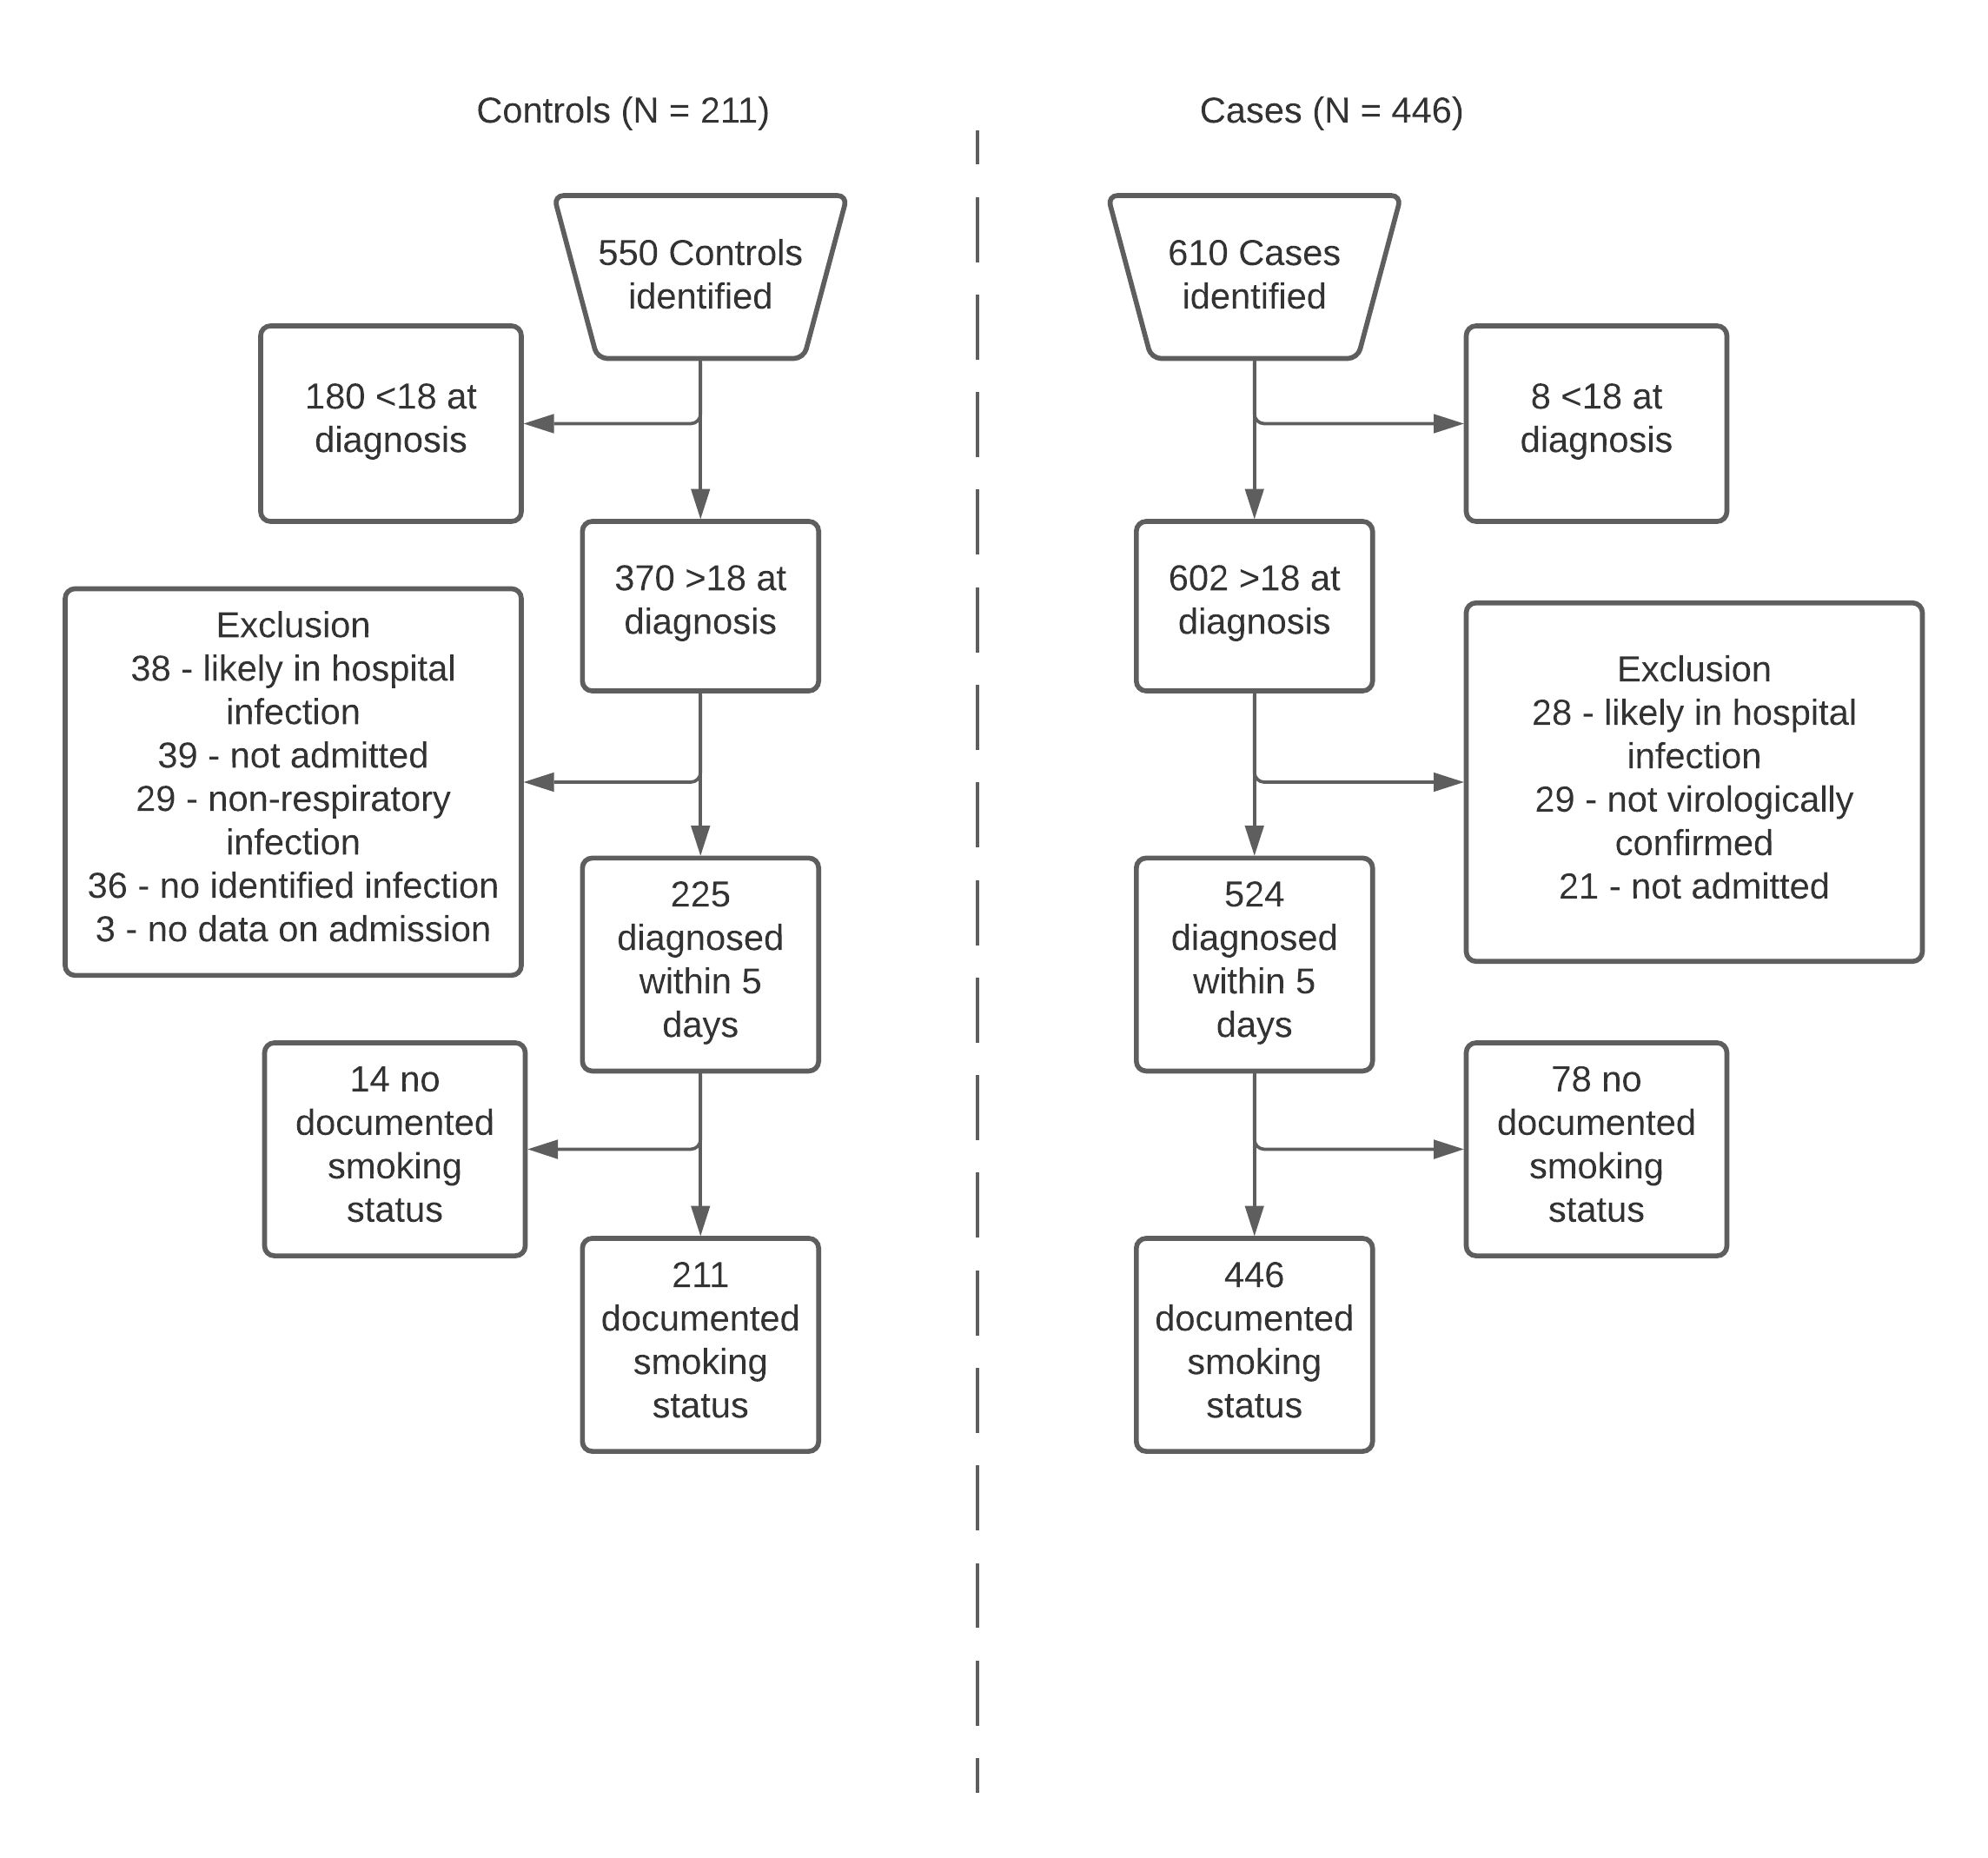
\includegraphics{figures/flow_diagram.png}
\caption{Eligibility flow diagram for controls and cases}
\end{figure}

\begin{center}\rule{0.5\linewidth}{0.5pt}\end{center}

A significantly larger proportion of cases compared with controls died
during their hospital admission (28.7\% vs.~4.3\%). For patients who
survived to discharge, the median length of hospital stay for cases and
controls was 9 (IQR = 4-18) and 4 (IQR = 2-9) days, respectively.

\hypertarget{table-1-population-characteristics}{%
\paragraph{Table 1: population
characteristics}\label{table-1-population-characteristics}}

\begin{Shaded}
\begin{Highlighting}[]
\KeywordTok{summary}\NormalTok{(t1, }\DataTypeTok{text =}\NormalTok{ T, }\DataTypeTok{labelTranslations =}\NormalTok{ mylabels, }\DataTypeTok{digits =} \DecValTok{2}\NormalTok{)}
\end{Highlighting}
\end{Shaded}

\begin{longtable}[]{@{}lcccr@{}}
\toprule
\begin{minipage}[b]{0.41\columnwidth}\raggedright
\strut
\end{minipage} & \begin{minipage}[b]{0.14\columnwidth}\centering
Controls (N=211)\strut
\end{minipage} & \begin{minipage}[b]{0.12\columnwidth}\centering
Cases (N=446)\strut
\end{minipage} & \begin{minipage}[b]{0.12\columnwidth}\centering
Total (N=657)\strut
\end{minipage} & \begin{minipage}[b]{0.06\columnwidth}\raggedleft
p value\strut
\end{minipage}\tabularnewline
\midrule
\endhead
\begin{minipage}[t]{0.41\columnwidth}\raggedright
Female\strut
\end{minipage} & \begin{minipage}[t]{0.14\columnwidth}\centering
116 (55.0\%)\strut
\end{minipage} & \begin{minipage}[t]{0.12\columnwidth}\centering
160 (35.9\%)\strut
\end{minipage} & \begin{minipage}[t]{0.12\columnwidth}\centering
276 (42.0\%)\strut
\end{minipage} & \begin{minipage}[t]{0.06\columnwidth}\raggedleft
\textless{} 0.001\strut
\end{minipage}\tabularnewline
\begin{minipage}[t]{0.41\columnwidth}\raggedright
Age\strut
\end{minipage} & \begin{minipage}[t]{0.14\columnwidth}\centering
\strut
\end{minipage} & \begin{minipage}[t]{0.12\columnwidth}\centering
\strut
\end{minipage} & \begin{minipage}[t]{0.12\columnwidth}\centering
\strut
\end{minipage} & \begin{minipage}[t]{0.06\columnwidth}\raggedleft
0.018\strut
\end{minipage}\tabularnewline
\begin{minipage}[t]{0.41\columnwidth}\raggedright
- Median\strut
\end{minipage} & \begin{minipage}[t]{0.14\columnwidth}\centering
62.46\strut
\end{minipage} & \begin{minipage}[t]{0.12\columnwidth}\centering
64.90\strut
\end{minipage} & \begin{minipage}[t]{0.12\columnwidth}\centering
64.58\strut
\end{minipage} & \begin{minipage}[t]{0.06\columnwidth}\raggedleft
\strut
\end{minipage}\tabularnewline
\begin{minipage}[t]{0.41\columnwidth}\raggedright
- Q1, Q3\strut
\end{minipage} & \begin{minipage}[t]{0.14\columnwidth}\centering
48.29, 75.74\strut
\end{minipage} & \begin{minipage}[t]{0.12\columnwidth}\centering
52.42, 76.20\strut
\end{minipage} & \begin{minipage}[t]{0.12\columnwidth}\centering
51.28, 76.12\strut
\end{minipage} & \begin{minipage}[t]{0.06\columnwidth}\raggedleft
\strut
\end{minipage}\tabularnewline
\begin{minipage}[t]{0.41\columnwidth}\raggedright
Categorical age\strut
\end{minipage} & \begin{minipage}[t]{0.14\columnwidth}\centering
\strut
\end{minipage} & \begin{minipage}[t]{0.12\columnwidth}\centering
\strut
\end{minipage} & \begin{minipage}[t]{0.12\columnwidth}\centering
\strut
\end{minipage} & \begin{minipage}[t]{0.06\columnwidth}\raggedleft
0.007\strut
\end{minipage}\tabularnewline
\begin{minipage}[t]{0.41\columnwidth}\raggedright
- 18-29\strut
\end{minipage} & \begin{minipage}[t]{0.14\columnwidth}\centering
18 (8.5\%)\strut
\end{minipage} & \begin{minipage}[t]{0.12\columnwidth}\centering
11 (2.5\%)\strut
\end{minipage} & \begin{minipage}[t]{0.12\columnwidth}\centering
29 (4.4\%)\strut
\end{minipage} & \begin{minipage}[t]{0.06\columnwidth}\raggedleft
\strut
\end{minipage}\tabularnewline
\begin{minipage}[t]{0.41\columnwidth}\raggedright
- 30-44\strut
\end{minipage} & \begin{minipage}[t]{0.14\columnwidth}\centering
22 (10.4\%)\strut
\end{minipage} & \begin{minipage}[t]{0.12\columnwidth}\centering
37 (8.3\%)\strut
\end{minipage} & \begin{minipage}[t]{0.12\columnwidth}\centering
59 (9.0\%)\strut
\end{minipage} & \begin{minipage}[t]{0.06\columnwidth}\raggedleft
\strut
\end{minipage}\tabularnewline
\begin{minipage}[t]{0.41\columnwidth}\raggedright
- 45-59\strut
\end{minipage} & \begin{minipage}[t]{0.14\columnwidth}\centering
46 (21.8\%)\strut
\end{minipage} & \begin{minipage}[t]{0.12\columnwidth}\centering
113 (25.3\%)\strut
\end{minipage} & \begin{minipage}[t]{0.12\columnwidth}\centering
159 (24.2\%)\strut
\end{minipage} & \begin{minipage}[t]{0.06\columnwidth}\raggedleft
\strut
\end{minipage}\tabularnewline
\begin{minipage}[t]{0.41\columnwidth}\raggedright
- 60-74\strut
\end{minipage} & \begin{minipage}[t]{0.14\columnwidth}\centering
67 (31.8\%)\strut
\end{minipage} & \begin{minipage}[t]{0.12\columnwidth}\centering
162 (36.3\%)\strut
\end{minipage} & \begin{minipage}[t]{0.12\columnwidth}\centering
229 (34.9\%)\strut
\end{minipage} & \begin{minipage}[t]{0.06\columnwidth}\raggedleft
\strut
\end{minipage}\tabularnewline
\begin{minipage}[t]{0.41\columnwidth}\raggedright
- 75+\strut
\end{minipage} & \begin{minipage}[t]{0.14\columnwidth}\centering
58 (27.5\%)\strut
\end{minipage} & \begin{minipage}[t]{0.12\columnwidth}\centering
123 (27.6\%)\strut
\end{minipage} & \begin{minipage}[t]{0.12\columnwidth}\centering
181 (27.5\%)\strut
\end{minipage} & \begin{minipage}[t]{0.06\columnwidth}\raggedleft
\strut
\end{minipage}\tabularnewline
\begin{minipage}[t]{0.41\columnwidth}\raggedright
Ethnicity\strut
\end{minipage} & \begin{minipage}[t]{0.14\columnwidth}\centering
\strut
\end{minipage} & \begin{minipage}[t]{0.12\columnwidth}\centering
\strut
\end{minipage} & \begin{minipage}[t]{0.12\columnwidth}\centering
\strut
\end{minipage} & \begin{minipage}[t]{0.06\columnwidth}\raggedleft
0.215\strut
\end{minipage}\tabularnewline
\begin{minipage}[t]{0.41\columnwidth}\raggedright
- Black British, Black African or Black Caribbean\strut
\end{minipage} & \begin{minipage}[t]{0.14\columnwidth}\centering
19 (9.0\%)\strut
\end{minipage} & \begin{minipage}[t]{0.12\columnwidth}\centering
63 (14.1\%)\strut
\end{minipage} & \begin{minipage}[t]{0.12\columnwidth}\centering
82 (12.5\%)\strut
\end{minipage} & \begin{minipage}[t]{0.06\columnwidth}\raggedleft
\strut
\end{minipage}\tabularnewline
\begin{minipage}[t]{0.41\columnwidth}\raggedright
- White British or White Other\strut
\end{minipage} & \begin{minipage}[t]{0.14\columnwidth}\centering
117 (55.5\%)\strut
\end{minipage} & \begin{minipage}[t]{0.12\columnwidth}\centering
220 (49.3\%)\strut
\end{minipage} & \begin{minipage}[t]{0.12\columnwidth}\centering
337 (51.3\%)\strut
\end{minipage} & \begin{minipage}[t]{0.06\columnwidth}\raggedleft
\strut
\end{minipage}\tabularnewline
\begin{minipage}[t]{0.41\columnwidth}\raggedright
- Not stated\strut
\end{minipage} & \begin{minipage}[t]{0.14\columnwidth}\centering
26 (12.3\%)\strut
\end{minipage} & \begin{minipage}[t]{0.12\columnwidth}\centering
43 (9.6\%)\strut
\end{minipage} & \begin{minipage}[t]{0.12\columnwidth}\centering
69 (10.5\%)\strut
\end{minipage} & \begin{minipage}[t]{0.06\columnwidth}\raggedleft
\strut
\end{minipage}\tabularnewline
\begin{minipage}[t]{0.41\columnwidth}\raggedright
- Asian British or Asian\strut
\end{minipage} & \begin{minipage}[t]{0.14\columnwidth}\centering
28 (13.3\%)\strut
\end{minipage} & \begin{minipage}[t]{0.12\columnwidth}\centering
68 (15.2\%)\strut
\end{minipage} & \begin{minipage}[t]{0.12\columnwidth}\centering
96 (14.6\%)\strut
\end{minipage} & \begin{minipage}[t]{0.06\columnwidth}\raggedleft
\strut
\end{minipage}\tabularnewline
\begin{minipage}[t]{0.41\columnwidth}\raggedright
- Other\strut
\end{minipage} & \begin{minipage}[t]{0.14\columnwidth}\centering
21 (10.0\%)\strut
\end{minipage} & \begin{minipage}[t]{0.12\columnwidth}\centering
52 (11.7\%)\strut
\end{minipage} & \begin{minipage}[t]{0.12\columnwidth}\centering
73 (11.1\%)\strut
\end{minipage} & \begin{minipage}[t]{0.06\columnwidth}\raggedleft
\strut
\end{minipage}\tabularnewline
\begin{minipage}[t]{0.41\columnwidth}\raggedright
IMD quintile\strut
\end{minipage} & \begin{minipage}[t]{0.14\columnwidth}\centering
\strut
\end{minipage} & \begin{minipage}[t]{0.12\columnwidth}\centering
\strut
\end{minipage} & \begin{minipage}[t]{0.12\columnwidth}\centering
\strut
\end{minipage} & \begin{minipage}[t]{0.06\columnwidth}\raggedleft
0.065\strut
\end{minipage}\tabularnewline
\begin{minipage}[t]{0.41\columnwidth}\raggedright
- Missing*\strut
\end{minipage} & \begin{minipage}[t]{0.14\columnwidth}\centering
5 (2.4\%)\strut
\end{minipage} & \begin{minipage}[t]{0.12\columnwidth}\centering
5 (1.1\%)\strut
\end{minipage} & \begin{minipage}[t]{0.12\columnwidth}\centering
10 (1.5\%)\strut
\end{minipage} & \begin{minipage}[t]{0.06\columnwidth}\raggedleft
\strut
\end{minipage}\tabularnewline
\begin{minipage}[t]{0.41\columnwidth}\raggedright
- 1 - Most deprived\strut
\end{minipage} & \begin{minipage}[t]{0.14\columnwidth}\centering
21 (10.0\%)\strut
\end{minipage} & \begin{minipage}[t]{0.12\columnwidth}\centering
26 (5.8\%)\strut
\end{minipage} & \begin{minipage}[t]{0.12\columnwidth}\centering
47 (7.2\%)\strut
\end{minipage} & \begin{minipage}[t]{0.06\columnwidth}\raggedleft
\strut
\end{minipage}\tabularnewline
\begin{minipage}[t]{0.41\columnwidth}\raggedright
- 2\strut
\end{minipage} & \begin{minipage}[t]{0.14\columnwidth}\centering
67 (31.8\%)\strut
\end{minipage} & \begin{minipage}[t]{0.12\columnwidth}\centering
121 (27.1\%)\strut
\end{minipage} & \begin{minipage}[t]{0.12\columnwidth}\centering
188 (28.6\%)\strut
\end{minipage} & \begin{minipage}[t]{0.06\columnwidth}\raggedleft
\strut
\end{minipage}\tabularnewline
\begin{minipage}[t]{0.41\columnwidth}\raggedright
- 3\strut
\end{minipage} & \begin{minipage}[t]{0.14\columnwidth}\centering
42 (19.9\%)\strut
\end{minipage} & \begin{minipage}[t]{0.12\columnwidth}\centering
122 (27.4\%)\strut
\end{minipage} & \begin{minipage}[t]{0.12\columnwidth}\centering
164 (25.0\%)\strut
\end{minipage} & \begin{minipage}[t]{0.06\columnwidth}\raggedleft
\strut
\end{minipage}\tabularnewline
\begin{minipage}[t]{0.41\columnwidth}\raggedright
- 4\strut
\end{minipage} & \begin{minipage}[t]{0.14\columnwidth}\centering
38 (18.0\%)\strut
\end{minipage} & \begin{minipage}[t]{0.12\columnwidth}\centering
98 (22.0\%)\strut
\end{minipage} & \begin{minipage}[t]{0.12\columnwidth}\centering
136 (20.7\%)\strut
\end{minipage} & \begin{minipage}[t]{0.06\columnwidth}\raggedleft
\strut
\end{minipage}\tabularnewline
\begin{minipage}[t]{0.41\columnwidth}\raggedright
- 5 - Least deprived\strut
\end{minipage} & \begin{minipage}[t]{0.14\columnwidth}\centering
38 (18.0\%)\strut
\end{minipage} & \begin{minipage}[t]{0.12\columnwidth}\centering
74 (16.6\%)\strut
\end{minipage} & \begin{minipage}[t]{0.12\columnwidth}\centering
112 (17.0\%)\strut
\end{minipage} & \begin{minipage}[t]{0.06\columnwidth}\raggedleft
\strut
\end{minipage}\tabularnewline
\begin{minipage}[t]{0.41\columnwidth}\raggedright
Smoking status\strut
\end{minipage} & \begin{minipage}[t]{0.14\columnwidth}\centering
\strut
\end{minipage} & \begin{minipage}[t]{0.12\columnwidth}\centering
\strut
\end{minipage} & \begin{minipage}[t]{0.12\columnwidth}\centering
\strut
\end{minipage} & \begin{minipage}[t]{0.06\columnwidth}\raggedleft
0.012\strut
\end{minipage}\tabularnewline
\begin{minipage}[t]{0.41\columnwidth}\raggedright
- Never smoker\strut
\end{minipage} & \begin{minipage}[t]{0.14\columnwidth}\centering
108 (51.2\%)\strut
\end{minipage} & \begin{minipage}[t]{0.12\columnwidth}\centering
232 (52.0\%)\strut
\end{minipage} & \begin{minipage}[t]{0.12\columnwidth}\centering
340 (51.8\%)\strut
\end{minipage} & \begin{minipage}[t]{0.06\columnwidth}\raggedleft
\strut
\end{minipage}\tabularnewline
\begin{minipage}[t]{0.41\columnwidth}\raggedright
- Former smoker\strut
\end{minipage} & \begin{minipage}[t]{0.14\columnwidth}\centering
67 (31.8\%)\strut
\end{minipage} & \begin{minipage}[t]{0.12\columnwidth}\centering
172 (38.6\%)\strut
\end{minipage} & \begin{minipage}[t]{0.12\columnwidth}\centering
239 (36.4\%)\strut
\end{minipage} & \begin{minipage}[t]{0.06\columnwidth}\raggedleft
\strut
\end{minipage}\tabularnewline
\begin{minipage}[t]{0.41\columnwidth}\raggedright
- Current smoker\strut
\end{minipage} & \begin{minipage}[t]{0.14\columnwidth}\centering
36 (17.1\%)\strut
\end{minipage} & \begin{minipage}[t]{0.12\columnwidth}\centering
42 (9.4\%)\strut
\end{minipage} & \begin{minipage}[t]{0.12\columnwidth}\centering
78 (11.9\%)\strut
\end{minipage} & \begin{minipage}[t]{0.06\columnwidth}\raggedleft
\strut
\end{minipage}\tabularnewline
\begin{minipage}[t]{0.41\columnwidth}\raggedright
System recorded smoking status\strut
\end{minipage} & \begin{minipage}[t]{0.14\columnwidth}\centering
\strut
\end{minipage} & \begin{minipage}[t]{0.12\columnwidth}\centering
\strut
\end{minipage} & \begin{minipage}[t]{0.12\columnwidth}\centering
\strut
\end{minipage} & \begin{minipage}[t]{0.06\columnwidth}\raggedleft
\textless{} 0.001\strut
\end{minipage}\tabularnewline
\begin{minipage}[t]{0.41\columnwidth}\raggedright
- Never smoker\strut
\end{minipage} & \begin{minipage}[t]{0.14\columnwidth}\centering
23 (10.9\%)\strut
\end{minipage} & \begin{minipage}[t]{0.12\columnwidth}\centering
233 (52.2\%)\strut
\end{minipage} & \begin{minipage}[t]{0.12\columnwidth}\centering
256 (39.0\%)\strut
\end{minipage} & \begin{minipage}[t]{0.06\columnwidth}\raggedleft
\strut
\end{minipage}\tabularnewline
\begin{minipage}[t]{0.41\columnwidth}\raggedright
- Former smoker\strut
\end{minipage} & \begin{minipage}[t]{0.14\columnwidth}\centering
22 (10.4\%)\strut
\end{minipage} & \begin{minipage}[t]{0.12\columnwidth}\centering
152 (34.1\%)\strut
\end{minipage} & \begin{minipage}[t]{0.12\columnwidth}\centering
174 (26.5\%)\strut
\end{minipage} & \begin{minipage}[t]{0.06\columnwidth}\raggedleft
\strut
\end{minipage}\tabularnewline
\begin{minipage}[t]{0.41\columnwidth}\raggedright
- Current smoker\strut
\end{minipage} & \begin{minipage}[t]{0.14\columnwidth}\centering
7 (3.3\%)\strut
\end{minipage} & \begin{minipage}[t]{0.12\columnwidth}\centering
30 (6.7\%)\strut
\end{minipage} & \begin{minipage}[t]{0.12\columnwidth}\centering
37 (5.6\%)\strut
\end{minipage} & \begin{minipage}[t]{0.06\columnwidth}\raggedleft
\strut
\end{minipage}\tabularnewline
\begin{minipage}[t]{0.41\columnwidth}\raggedright
- Unknown\strut
\end{minipage} & \begin{minipage}[t]{0.14\columnwidth}\centering
159 (75.4\%)\strut
\end{minipage} & \begin{minipage}[t]{0.12\columnwidth}\centering
31 (7.0\%)\strut
\end{minipage} & \begin{minipage}[t]{0.12\columnwidth}\centering
190 (28.9\%)\strut
\end{minipage} & \begin{minipage}[t]{0.06\columnwidth}\raggedleft
\strut
\end{minipage}\tabularnewline
\begin{minipage}[t]{0.41\columnwidth}\raggedright
Survival to discharge\strut
\end{minipage} & \begin{minipage}[t]{0.14\columnwidth}\centering
202 (95.7\%)\strut
\end{minipage} & \begin{minipage}[t]{0.12\columnwidth}\centering
318 (71.3\%)\strut
\end{minipage} & \begin{minipage}[t]{0.12\columnwidth}\centering
520 (79.1\%)\strut
\end{minipage} & \begin{minipage}[t]{0.06\columnwidth}\raggedleft
\textless{} 0.001\strut
\end{minipage}\tabularnewline
\begin{minipage}[t]{0.41\columnwidth}\raggedright
Length of admission for survivors (days)\strut
\end{minipage} & \begin{minipage}[t]{0.14\columnwidth}\centering
\strut
\end{minipage} & \begin{minipage}[t]{0.12\columnwidth}\centering
\strut
\end{minipage} & \begin{minipage}[t]{0.12\columnwidth}\centering
\strut
\end{minipage} & \begin{minipage}[t]{0.06\columnwidth}\raggedleft
\textless{} 0.001\strut
\end{minipage}\tabularnewline
\begin{minipage}[t]{0.41\columnwidth}\raggedright
- Median\strut
\end{minipage} & \begin{minipage}[t]{0.14\columnwidth}\centering
4.00\strut
\end{minipage} & \begin{minipage}[t]{0.12\columnwidth}\centering
9.00\strut
\end{minipage} & \begin{minipage}[t]{0.12\columnwidth}\centering
7.00\strut
\end{minipage} & \begin{minipage}[t]{0.06\columnwidth}\raggedleft
\strut
\end{minipage}\tabularnewline
\begin{minipage}[t]{0.41\columnwidth}\raggedright
- Q1, Q3\strut
\end{minipage} & \begin{minipage}[t]{0.14\columnwidth}\centering
2.00, 9.00\strut
\end{minipage} & \begin{minipage}[t]{0.12\columnwidth}\centering
4.00, 18.00\strut
\end{minipage} & \begin{minipage}[t]{0.12\columnwidth}\centering
3.00, 14.00\strut
\end{minipage} & \begin{minipage}[t]{0.06\columnwidth}\raggedleft
\strut
\end{minipage}\tabularnewline
\begin{minipage}[t]{0.41\columnwidth}\raggedright
Cancer (current or past)\strut
\end{minipage} & \begin{minipage}[t]{0.14\columnwidth}\centering
65 (30.8\%)\strut
\end{minipage} & \begin{minipage}[t]{0.12\columnwidth}\centering
90 (20.2\%)\strut
\end{minipage} & \begin{minipage}[t]{0.12\columnwidth}\centering
155 (23.6\%)\strut
\end{minipage} & \begin{minipage}[t]{0.06\columnwidth}\raggedleft
0.003\strut
\end{minipage}\tabularnewline
\begin{minipage}[t]{0.41\columnwidth}\raggedright
Auto-immune disease (present)\strut
\end{minipage} & \begin{minipage}[t]{0.14\columnwidth}\centering
12 (5.7\%)\strut
\end{minipage} & \begin{minipage}[t]{0.12\columnwidth}\centering
16 (3.6\%)\strut
\end{minipage} & \begin{minipage}[t]{0.12\columnwidth}\centering
28 (4.3\%)\strut
\end{minipage} & \begin{minipage}[t]{0.06\columnwidth}\raggedleft
0.213\strut
\end{minipage}\tabularnewline
\begin{minipage}[t]{0.41\columnwidth}\raggedright
Metabolic disease (present)\strut
\end{minipage} & \begin{minipage}[t]{0.14\columnwidth}\centering
28 (13.3\%)\strut
\end{minipage} & \begin{minipage}[t]{0.12\columnwidth}\centering
135 (30.3\%)\strut
\end{minipage} & \begin{minipage}[t]{0.12\columnwidth}\centering
163 (24.8\%)\strut
\end{minipage} & \begin{minipage}[t]{0.06\columnwidth}\raggedleft
\textless{} 0.001\strut
\end{minipage}\tabularnewline
\begin{minipage}[t]{0.41\columnwidth}\raggedright
Haematological disease (present)\strut
\end{minipage} & \begin{minipage}[t]{0.14\columnwidth}\centering
3 (1.4\%)\strut
\end{minipage} & \begin{minipage}[t]{0.12\columnwidth}\centering
4 (0.9\%)\strut
\end{minipage} & \begin{minipage}[t]{0.12\columnwidth}\centering
7 (1.1\%)\strut
\end{minipage} & \begin{minipage}[t]{0.06\columnwidth}\raggedleft
0.541\strut
\end{minipage}\tabularnewline
\begin{minipage}[t]{0.41\columnwidth}\raggedright
Cardiac disease (present)\strut
\end{minipage} & \begin{minipage}[t]{0.14\columnwidth}\centering
64 (30.3\%)\strut
\end{minipage} & \begin{minipage}[t]{0.12\columnwidth}\centering
238 (53.4\%)\strut
\end{minipage} & \begin{minipage}[t]{0.12\columnwidth}\centering
302 (46.0\%)\strut
\end{minipage} & \begin{minipage}[t]{0.06\columnwidth}\raggedleft
\textless{} 0.001\strut
\end{minipage}\tabularnewline
\begin{minipage}[t]{0.41\columnwidth}\raggedright
Neurological disease (present)\strut
\end{minipage} & \begin{minipage}[t]{0.14\columnwidth}\centering
25 (11.8\%)\strut
\end{minipage} & \begin{minipage}[t]{0.12\columnwidth}\centering
54 (12.1\%)\strut
\end{minipage} & \begin{minipage}[t]{0.12\columnwidth}\centering
79 (12.0\%)\strut
\end{minipage} & \begin{minipage}[t]{0.06\columnwidth}\raggedleft
0.924\strut
\end{minipage}\tabularnewline
\begin{minipage}[t]{0.41\columnwidth}\raggedright
Respiratory disease (present)\strut
\end{minipage} & \begin{minipage}[t]{0.14\columnwidth}\centering
54 (25.6\%)\strut
\end{minipage} & \begin{minipage}[t]{0.12\columnwidth}\centering
91 (20.4\%)\strut
\end{minipage} & \begin{minipage}[t]{0.12\columnwidth}\centering
145 (22.1\%)\strut
\end{minipage} & \begin{minipage}[t]{0.06\columnwidth}\raggedleft
0.134\strut
\end{minipage}\tabularnewline
\begin{minipage}[t]{0.41\columnwidth}\raggedright
Renal disease (present)\strut
\end{minipage} & \begin{minipage}[t]{0.14\columnwidth}\centering
12 (5.7\%)\strut
\end{minipage} & \begin{minipage}[t]{0.12\columnwidth}\centering
37 (8.3\%)\strut
\end{minipage} & \begin{minipage}[t]{0.12\columnwidth}\centering
49 (7.5\%)\strut
\end{minipage} & \begin{minipage}[t]{0.06\columnwidth}\raggedleft
0.235\strut
\end{minipage}\tabularnewline
\begin{minipage}[t]{0.41\columnwidth}\raggedright
HIV (present)\strut
\end{minipage} & \begin{minipage}[t]{0.14\columnwidth}\centering
2 (0.9\%)\strut
\end{minipage} & \begin{minipage}[t]{0.12\columnwidth}\centering
7 (1.6\%)\strut
\end{minipage} & \begin{minipage}[t]{0.12\columnwidth}\centering
9 (1.4\%)\strut
\end{minipage} & \begin{minipage}[t]{0.06\columnwidth}\raggedleft
0.522\strut
\end{minipage}\tabularnewline
\begin{minipage}[t]{0.41\columnwidth}\raggedright
No relevant comorbidities\strut
\end{minipage} & \begin{minipage}[t]{0.14\columnwidth}\centering
43 (20.4\%)\strut
\end{minipage} & \begin{minipage}[t]{0.12\columnwidth}\centering
85 (19.1\%)\strut
\end{minipage} & \begin{minipage}[t]{0.12\columnwidth}\centering
128 (19.5\%)\strut
\end{minipage} & \begin{minipage}[t]{0.06\columnwidth}\raggedleft
0.690\strut
\end{minipage}\tabularnewline
\bottomrule
\end{longtable}

\begin{Shaded}
\begin{Highlighting}[]
\NormalTok{pack_year <-}\StringTok{ }\KeywordTok{bind_rows}\NormalTok{(cases, controls) }\OperatorTok
\StringTok{  }\KeywordTok{drop_na}\NormalTok{(pack_years) }\OperatorTok
\StringTok{  }\KeywordTok{filter}\NormalTok{(}\OperatorTok{!}\NormalTok{pack_years }\OperatorTok\StringTok{ }\KeywordTok{c}\NormalTok{(}\StringTok{"nil"}\NormalTok{, }\StringTok{"na"}\NormalTok{, }\StringTok{"no_information"}\NormalTok{, }\StringTok{"not_recorded"}\NormalTok{)) }\OperatorTok
\StringTok{  }\KeywordTok{group_by}\NormalTok{(cohort, smoking_status) }\OperatorTok
\StringTok{  }\KeywordTok{mutate}\NormalTok{(}\DataTypeTok{pack_years =} \KeywordTok{as.numeric}\NormalTok{(pack_years)) }\OperatorTok
\StringTok{  }\KeywordTok{summarise}\NormalTok{(}\DataTypeTok{med_py =} \KeywordTok{median}\NormalTok{(pack_years),}
            \DataTypeTok{x =} \KeywordTok{quantile}\NormalTok{(pack_years, }\KeywordTok{c}\NormalTok{(}\FloatTok{0.25}\NormalTok{, }\FloatTok{0.75}\NormalTok{)))}
\end{Highlighting}
\end{Shaded}

*\textsuperscript{``IMD values are not available for individuals with
home addresses outside of the UK''}

\begin{center}\rule{0.5\linewidth}{0.5pt}\end{center}

Controls and cases were predominantly admitted from North central and
North East central London (see Figure 2). The number of cases admitted
from peripheral locations was higher than in controls and represents
transfer of inpatients from other hospitals and diversion of patients
that would otherwise have attended local hospitals due to bed pressures.

\hypertarget{figure-2-patients-home-addresses-in-london}{%
\paragraph{Figure 2: patients home addresses in
London}\label{figure-2-patients-home-addresses-in-london}}

\begin{figure}
\centering
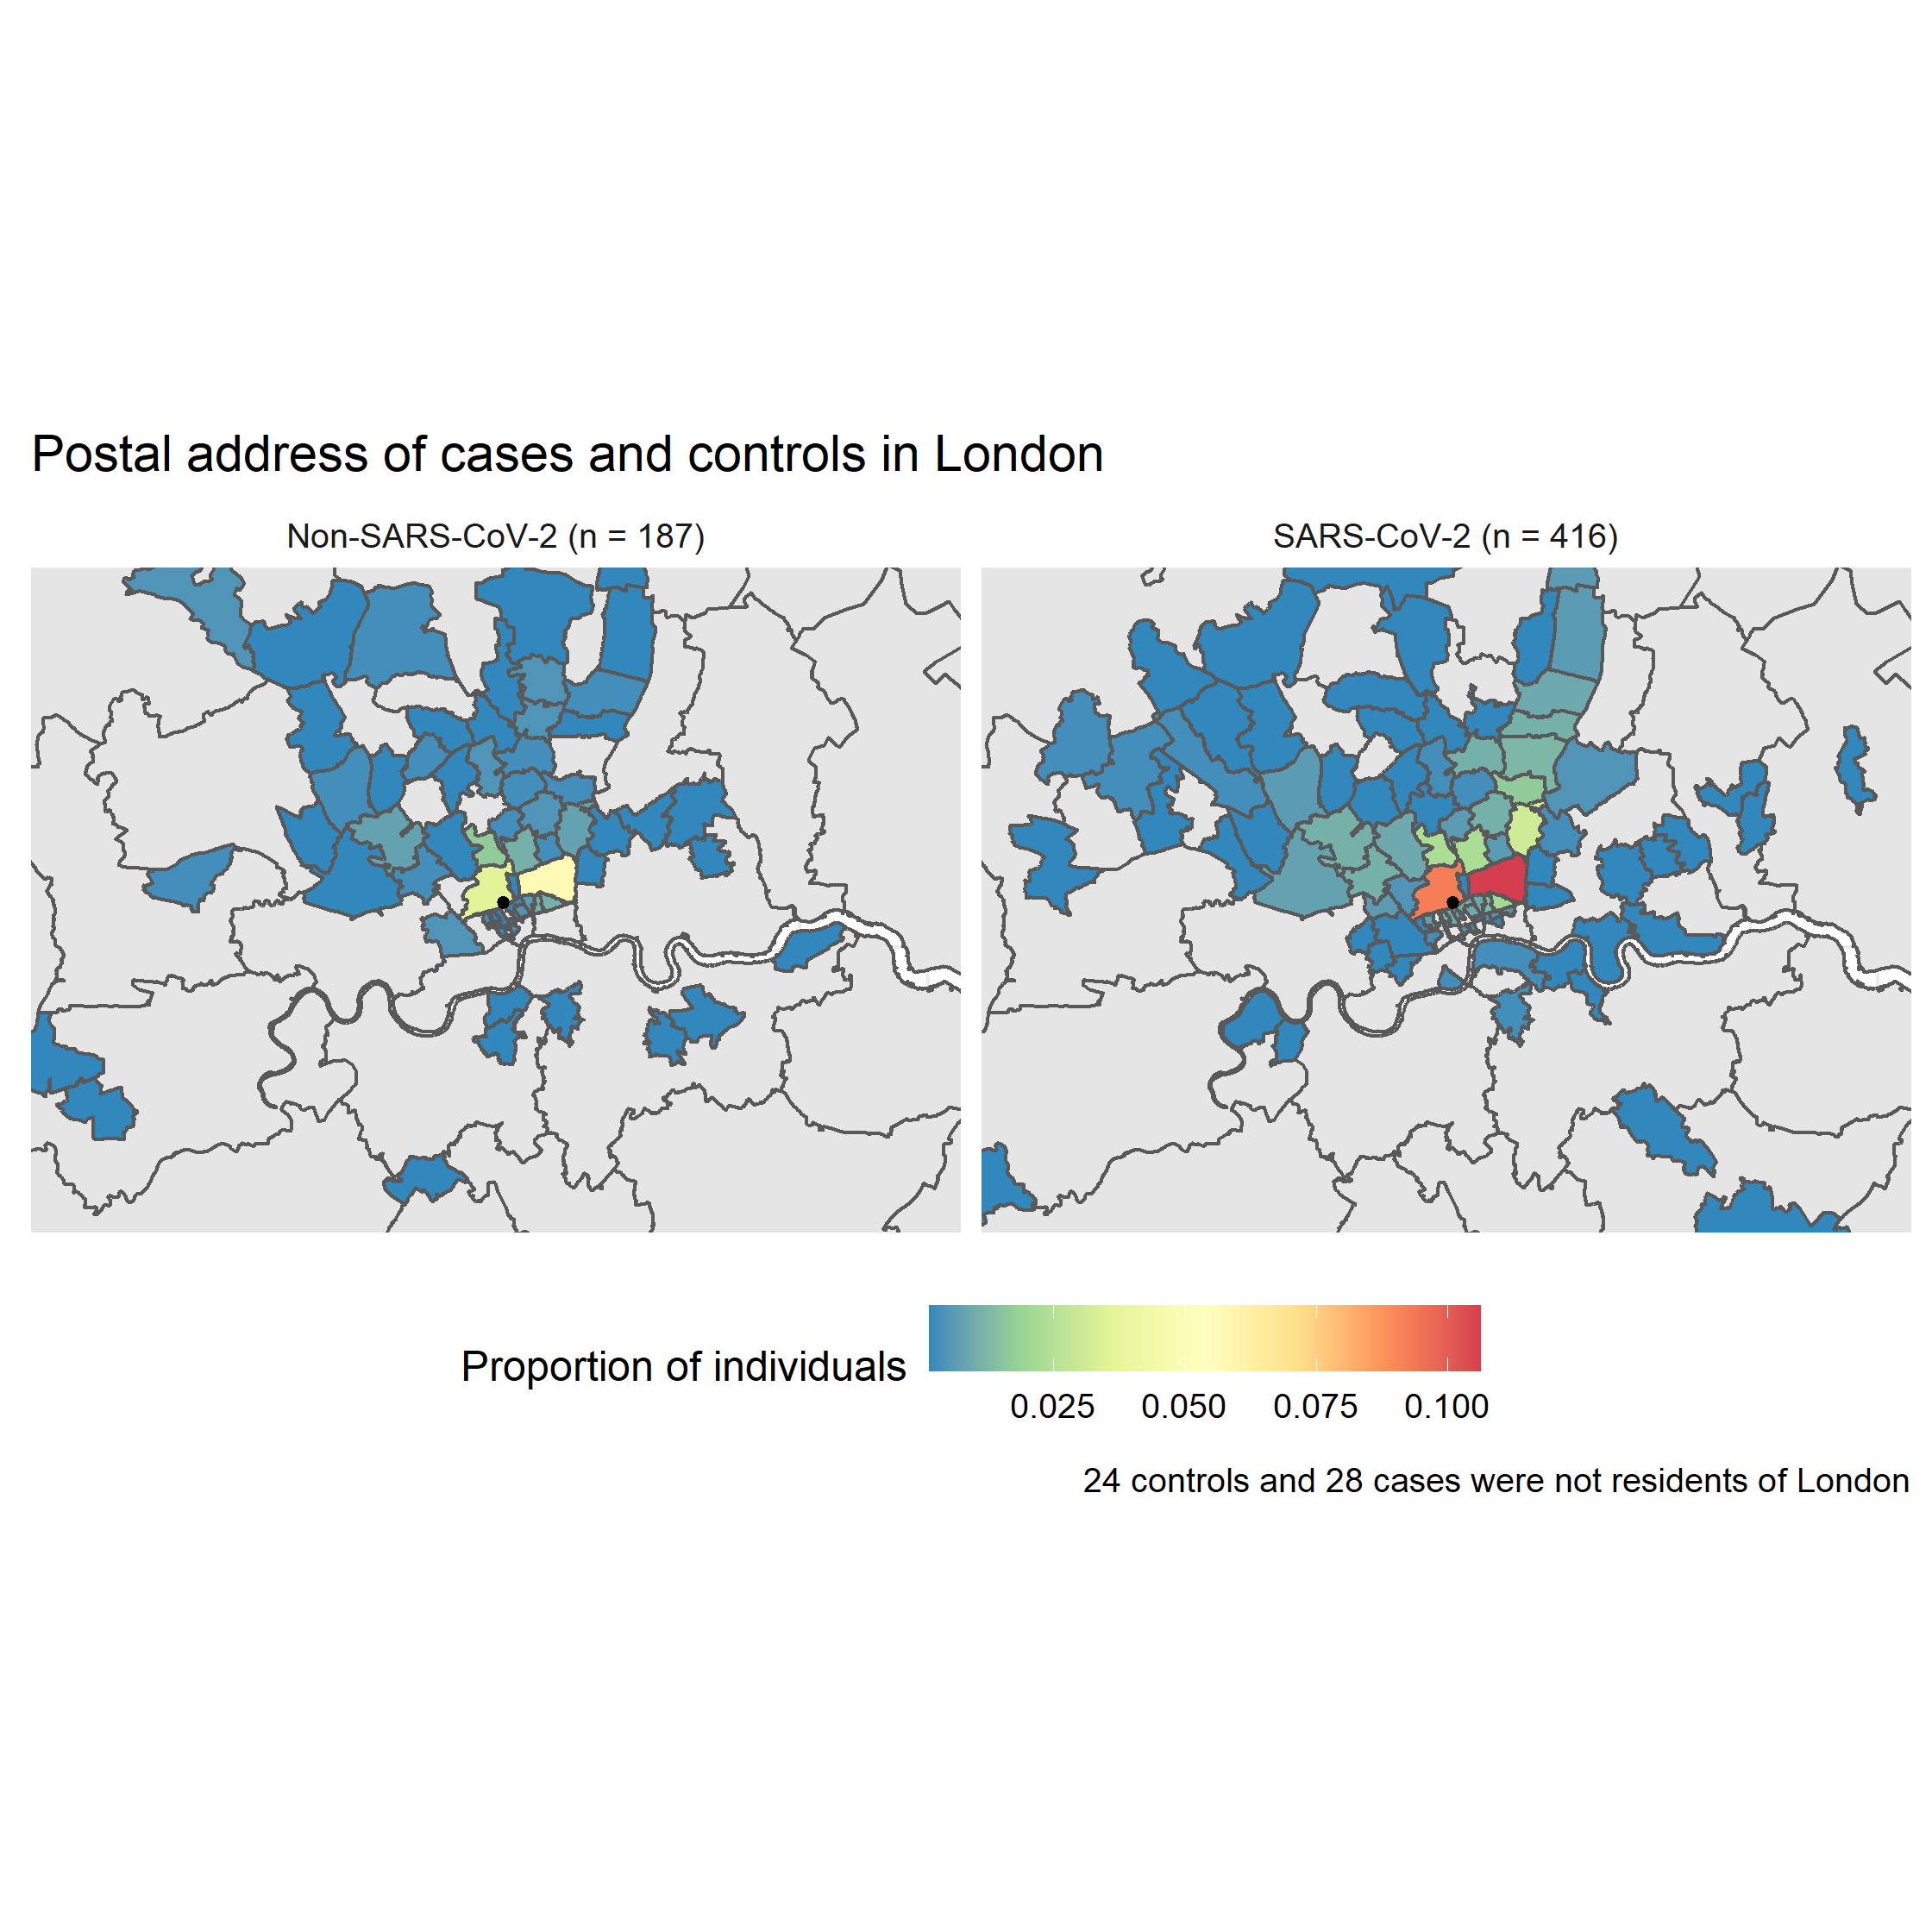
\includegraphics{figures/higher_level_map.png}
\caption{Postal district level map of London}
\end{figure}

\begin{center}\rule{0.5\linewidth}{0.5pt}\end{center}

\hypertarget{association-of-smoking-status-with-type-of-hospitalisation}{%
\paragraph{\texorpdfstring{\emph{Association of smoking status with type
of hospitalisation
}}{Association of smoking status with type of hospitalisation }}\label{association-of-smoking-status-with-type-of-hospitalisation}}

The prevalence of former smoking was higher in cases compared with
controls (38.6\% vs.~31.8\%). Current smoking prevalence was higher in
controls compared with cases (17.1\% vs.~9.4\%). A single patient from
the case cohort was recorded as a dual cigarette and e-cigarette user.
Two patients, one from each cohort, were recorded as dual cigarette and
shisha/waterpipe users.

In the univariable analysis, current smokers had significantly reduced
odds of being hospitalised with COVID-19 compared with other respiratory
viruses (OR = 0.52, 95\% CI = 0.31-0.86, \emph{p} = 0.01). The odds for
former smokers were equivocal (OR = 1.16, 95\% CI = 0.81-1.68, \emph{p}
= 0.43).

In the multivariable analysis adjusted for sex, age, socioeconomic
position and comorbidities, current smokers had significantly reduced
odds of being hospitalised with COVID-19 compared with other respiratory
viruses (OR = 0.55, 95\% CI = 0.31-0.96, \emph{p} = 0.04). The odds for
former smokers were equivocal (OR = 1.08, 95\% C.I. = 0.72-1.61,
\emph{p} = 0.70).

\begin{Shaded}
\begin{Highlighting}[]
\NormalTok{a <-}\StringTok{ }\KeywordTok{cbind}\NormalTok{(}\KeywordTok{exp}\NormalTok{(}\KeywordTok{cbind}\NormalTok{(}\DataTypeTok{OR =} \KeywordTok{coef}\NormalTok{(unadjusted), }\KeywordTok{confint}\NormalTok{(unadjusted))), }\DataTypeTok{p =} \KeywordTok{round}\NormalTok{(}\KeywordTok{summary}\NormalTok{(unadjusted)}\OperatorTok{$}\NormalTok{coefficients[,}\DecValTok{4}\NormalTok{], }\DecValTok{3}\NormalTok{))}
\KeywordTok{kable}\NormalTok{(a[}\DecValTok{2}\OperatorTok{:}\DecValTok{3}\NormalTok{,] }\OperatorTok
\StringTok{  }\KeywordTok{as_tibble}\NormalTok{() }\OperatorTok
\StringTok{  }\KeywordTok{cbind}\NormalTok{(}\StringTok{"Smoking status"}\NormalTok{ =}\StringTok{ }\KeywordTok{c}\NormalTok{(}\StringTok{"Former smoker"}\NormalTok{, }\StringTok{"Current smoker"}\NormalTok{)) }\OperatorTok
\StringTok{  }\KeywordTok{mutate}\NormalTok{(}\DataTypeTok{OR =} \KeywordTok{round}\NormalTok{(OR, }\DecValTok{2}\NormalTok{),}
         \StringTok{`}\DataTypeTok{2.5 %}\StringTok{`}\NormalTok{ =}\StringTok{ }\KeywordTok{round}\NormalTok{(}\StringTok{`}\DataTypeTok{2.5 %}\StringTok{`}\NormalTok{, }\DecValTok{2}\NormalTok{),}
         \StringTok{`}\DataTypeTok{97.5 %}\StringTok{`}\NormalTok{ =}\StringTok{ }\KeywordTok{round}\NormalTok{(}\StringTok{`}\DataTypeTok{97.5 %}\StringTok{`}\NormalTok{, }\DecValTok{2}\NormalTok{),}
         \DataTypeTok{p =} \KeywordTok{round}\NormalTok{(p, }\DecValTok{2}\NormalTok{)) }\OperatorTok
\StringTok{  }\KeywordTok{rename}\NormalTok{(}\StringTok{"Odds ratio"}\NormalTok{ =}\StringTok{ }\DecValTok{1}\NormalTok{, }\StringTok{"2.5% CI"}\NormalTok{ =}\StringTok{ }\DecValTok{2}\NormalTok{, }\StringTok{"97.5% CI"}\NormalTok{ =}\StringTok{ }\DecValTok{3}\NormalTok{, }\StringTok{"p"}\NormalTok{ =}\StringTok{ }\DecValTok{4}\NormalTok{) }\OperatorTok
\StringTok{  }\KeywordTok{select}\NormalTok{(}\KeywordTok{c}\NormalTok{(}\StringTok{"Smoking status"}\NormalTok{, }\StringTok{"Odds ratio"}\NormalTok{, }\StringTok{"2.5% CI"}\NormalTok{, }\StringTok{"97.5% CI"}\NormalTok{, }\StringTok{"p"}\NormalTok{)))}
\end{Highlighting}
\end{Shaded}

\begin{longtable}[]{@{}lrrrr@{}}
\toprule
Smoking status & Odds ratio & 2.5\% CI & 97.5\% CI & p\tabularnewline
\midrule
\endhead
Former smoker & 1.16 & 0.81 & 1.68 & 0.43\tabularnewline
Current smoker & 0.52 & 0.31 & 0.86 & 0.01\tabularnewline
\bottomrule
\end{longtable}

\begin{Shaded}
\begin{Highlighting}[]
\NormalTok{a <-}\StringTok{ }\KeywordTok{cbind}\NormalTok{(}\KeywordTok{exp}\NormalTok{(}\KeywordTok{cbind}\NormalTok{(}\DataTypeTok{OR =} \KeywordTok{coef}\NormalTok{(fully_adjusted), }\KeywordTok{confint}\NormalTok{(fully_adjusted))), }\DataTypeTok{p =} \KeywordTok{round}\NormalTok{(}\KeywordTok{summary}\NormalTok{(fully_adjusted)}\OperatorTok{$}\NormalTok{coefficients[,}\DecValTok{4}\NormalTok{], }\DecValTok{3}\NormalTok{))}
\KeywordTok{kable}\NormalTok{(a[}\DecValTok{2}\OperatorTok{:}\DecValTok{3}\NormalTok{,] }\OperatorTok
\StringTok{  }\KeywordTok{as_tibble}\NormalTok{() }\OperatorTok
\StringTok{  }\KeywordTok{cbind}\NormalTok{(}\StringTok{"Smoking status"}\NormalTok{ =}\StringTok{ }\KeywordTok{c}\NormalTok{(}\StringTok{"Former smoker"}\NormalTok{, }\StringTok{"Current smoker"}\NormalTok{)) }\OperatorTok
\StringTok{  }\KeywordTok{mutate}\NormalTok{(}\DataTypeTok{OR =} \KeywordTok{round}\NormalTok{(OR, }\DecValTok{2}\NormalTok{),}
         \StringTok{`}\DataTypeTok{2.5 %}\StringTok{`}\NormalTok{ =}\StringTok{ }\KeywordTok{round}\NormalTok{(}\StringTok{`}\DataTypeTok{2.5 %}\StringTok{`}\NormalTok{, }\DecValTok{2}\NormalTok{),}
         \StringTok{`}\DataTypeTok{97.5 %}\StringTok{`}\NormalTok{ =}\StringTok{ }\KeywordTok{round}\NormalTok{(}\StringTok{`}\DataTypeTok{97.5 %}\StringTok{`}\NormalTok{, }\DecValTok{2}\NormalTok{),}
         \DataTypeTok{p =} \KeywordTok{round}\NormalTok{(p, }\DecValTok{2}\NormalTok{)) }\OperatorTok
\StringTok{  }\KeywordTok{rename}\NormalTok{(}\StringTok{"Adjusted odds ratio"}\NormalTok{ =}\StringTok{ }\DecValTok{1}\NormalTok{, }\StringTok{"2.5% CI"}\NormalTok{ =}\StringTok{ }\DecValTok{2}\NormalTok{, }\StringTok{"97.5% CI"}\NormalTok{ =}\StringTok{ }\DecValTok{3}\NormalTok{, }\StringTok{"p"}\NormalTok{ =}\StringTok{ }\DecValTok{4}\NormalTok{) }\OperatorTok
\StringTok{  }\KeywordTok{select}\NormalTok{(}\KeywordTok{c}\NormalTok{(}\StringTok{"Smoking status"}\NormalTok{, }\StringTok{"Adjusted odds ratio"}\NormalTok{, }\StringTok{"2.5% CI"}\NormalTok{, }\StringTok{"97.5% CI"}\NormalTok{, }\StringTok{"p"}\NormalTok{)))}
\end{Highlighting}
\end{Shaded}

\begin{longtable}[]{@{}lrrrr@{}}
\toprule
Smoking status & Adjusted odds ratio & 2.5\% CI & 97.5\% CI &
p\tabularnewline
\midrule
\endhead
Former smoker & 1.08 & 0.71 & 1.65 & 0.71\tabularnewline
Current smoker & 0.55 & 0.31 & 0.97 & 0.04\tabularnewline
\bottomrule
\end{longtable}

\hypertarget{sensitivity-analysis}{%
\paragraph{\texorpdfstring{\emph{Sensitivity
analysis}}{Sensitivity analysis}}\label{sensitivity-analysis}}

In the sensitivity analysis with individuals recorded as non-smokers
excluded from the sample (leaving 159 controls and 398 cases), current
smokers had significantly reduced odds of being hospitalised with
COVID-19 compared with other respiratory viruses (OR = 0.41, 95\% CI =
0.22-0.74, \emph{p} = 0.03). The odds for former smokers were equivocal
(OR = 0.78, 95\% C.I. = 0.49-1.23, \emph{p} = 0.28).

In exploratory, age-stratified analyses, there was no evidence of lower
than expected current smoking prevalence in controls compared with
overall London prevalence (see Table 2). In cases, however, current
smoking in those aged 45-59 years was significantly lower than expected
on the basis of age-matched London prevalence (4.5\% vs.~13.8\%,
\emph{p} = 0.003).

\hypertarget{proportion-z-tests-comparing-smoking-among-cases-and-controls-to-london-prevalence}{%
\subsection{Proportion Z-tests comparing smoking among cases and
controls to London
prevalence}\label{proportion-z-tests-comparing-smoking-among-cases-and-controls-to-london-prevalence}}

\begin{Shaded}
\begin{Highlighting}[]
\KeywordTok{source}\NormalTok{(}\KeywordTok{here}\NormalTok{(}\StringTok{"scripts"}\NormalTok{, }\StringTok{"crosstab_functions.R"}\NormalTok{))}
\NormalTok{xtable <-}\StringTok{ }\KeywordTok{crosstab}\NormalTok{(smoking_proportions, }\DataTypeTok{row.vars =} \KeywordTok{c}\NormalTok{(}\StringTok{"aps_age"}\NormalTok{), }\DataTypeTok{col.vars =} \KeywordTok{c}\NormalTok{(}\StringTok{"cohort"}\NormalTok{,}\StringTok{"smoking_status"}\NormalTok{), }\DataTypeTok{type =} \KeywordTok{c}\NormalTok{(}\StringTok{"f"}\NormalTok{,}\StringTok{"r"}\NormalTok{), }\DataTypeTok{dec.places =} \DecValTok{1}\NormalTok{)}

\NormalTok{weighting <-}\StringTok{ }\NormalTok{smoking_proportions }\OperatorTok
\StringTok{  }\KeywordTok{ungroup}\NormalTok{() }\OperatorTok
\StringTok{  }\KeywordTok{filter}\NormalTok{(cohort }\OperatorTok{==}\StringTok{ "cases"}\NormalTok{) }\OperatorTok
\StringTok{  }\KeywordTok{select}\NormalTok{(aps_age, sex) }\OperatorTok
\StringTok{  }\KeywordTok{group_by_all}\NormalTok{() }\OperatorTok
\StringTok{  }\KeywordTok{summarise}\NormalTok{(}\DataTypeTok{n =} \KeywordTok{n}\NormalTok{()) }\OperatorTok
\StringTok{  }\KeywordTok{mutate}\NormalTok{(}\DataTypeTok{proportion =}\NormalTok{ n}\OperatorTok{/}\KeywordTok{sum}\NormalTok{(n))}

\NormalTok{weighted_mean <-}\StringTok{ }\NormalTok{london_xtab }\OperatorTok
\StringTok{  }\KeywordTok{mutate}\NormalTok{(}\DataTypeTok{aps_age =} \KeywordTok{recode}\NormalTok{(aps_age, }
                          \StringTok{"18_29"}\NormalTok{ =}\StringTok{ "18-29"}\NormalTok{,}
                          \StringTok{"30_44"}\NormalTok{ =}\StringTok{ "30-44"}\NormalTok{,}
                          \StringTok{"45_59"}\NormalTok{ =}\StringTok{ "45-59"}\NormalTok{,}
                          \StringTok{"60_74"}\NormalTok{ =}\StringTok{ "60-74"}\NormalTok{)) }\OperatorTok
\StringTok{  }\KeywordTok{left_join}\NormalTok{(., weighting) }\OperatorTok
\StringTok{  }\KeywordTok{mutate}\NormalTok{(}\DataTypeTok{weighted_percentage =}\NormalTok{ percentage }\OperatorTok{*}\StringTok{ }\NormalTok{proportion) }\OperatorTok
\StringTok{  }\KeywordTok{ungroup}\NormalTok{() }\OperatorTok
\StringTok{  }\KeywordTok{group_by}\NormalTok{(smoking_status, aps_age) }\OperatorTok
\StringTok{  }\KeywordTok{summarise}\NormalTok{(}\DataTypeTok{weighted_percentage =} \KeywordTok{sum}\NormalTok{(weighted_percentage)) }\OperatorTok
\StringTok{  }\KeywordTok{mutate}\NormalTok{(}\DataTypeTok{cohort =} \StringTok{"london"}\NormalTok{)}

\KeywordTok{read_xlsx}\NormalTok{(}\KeywordTok{here}\NormalTok{(}\StringTok{"clean_data"}\NormalTok{, }\StringTok{"smoking_table.xlsx"}\NormalTok{)) }\OperatorTok
\StringTok{  }\KeywordTok{drop_na}\NormalTok{() }\OperatorTok
\StringTok{  }\KeywordTok{select}\NormalTok{(}\DecValTok{1}\OperatorTok{:}\DecValTok{10}\NormalTok{) }\OperatorTok
\StringTok{  }\KeywordTok{mutate}\NormalTok{(}\DataTypeTok{london_current_smoker =} \KeywordTok{paste}\NormalTok{(london_current_smoker}\OperatorTok{*}\DecValTok{100}\NormalTok{, }\StringTok{"%"}\NormalTok{, }\DataTypeTok{sep =} \StringTok{""}\NormalTok{),}
         \DataTypeTok{london_former_smoker =} \KeywordTok{paste}\NormalTok{(london_former_smoker}\OperatorTok{*}\DecValTok{100}\NormalTok{, }\StringTok{"%"}\NormalTok{, }\DataTypeTok{sep =} \StringTok{""}\NormalTok{),}
         \DataTypeTok{london_never_smoker =} \KeywordTok{paste}\NormalTok{(london_never_smoker}\OperatorTok{*}\DecValTok{100}\NormalTok{, }\StringTok{"%"}\NormalTok{, }\DataTypeTok{sep =} \StringTok{""}\NormalTok{),}
         \DataTypeTok{age =} \KeywordTok{recode}\NormalTok{(age, }\StringTok{"18_29"}\NormalTok{ =}\StringTok{ "18-29"}\NormalTok{,}
                      \StringTok{"30_44"}\NormalTok{ =}\StringTok{ "30-44"}\NormalTok{,}
                      \StringTok{"45_59"}\NormalTok{ =}\StringTok{ "40-59"}\NormalTok{,}
                      \StringTok{"60_74"}\NormalTok{ =}\StringTok{ "60-74"}\NormalTok{)) }\OperatorTok
\StringTok{  }\KeywordTok{flextable}\NormalTok{() }\OperatorTok
\StringTok{  }\KeywordTok{set_header_labels}\NormalTok{(.,}
                    \DataTypeTok{values =} \KeywordTok{list}\NormalTok{(}\DataTypeTok{age =} \StringTok{"Age"}\NormalTok{,}
                                  \DataTypeTok{controls_current_smoker =} \StringTok{"Current smoker"}\NormalTok{,}
                                  \DataTypeTok{controls_former_smoker =}\StringTok{"Former smoker"}\NormalTok{,}
                                  \DataTypeTok{controls_never_smoker =} \StringTok{"Never smoker"}\NormalTok{,}
                                  \DataTypeTok{cases_current_smoker =} \StringTok{"Current smoker"}\NormalTok{,}
                                  \DataTypeTok{cases_former_smoker =} \StringTok{"Former smoker"}\NormalTok{,}
                                  \DataTypeTok{cases_never_smoker =} \StringTok{"Never smoker"}\NormalTok{,}
                                  \DataTypeTok{london_current_smoker =} \StringTok{"Current smoker"}\NormalTok{,}
                                  \DataTypeTok{london_former_smoker =} \StringTok{"Former smoker"}\NormalTok{,}
                                  \DataTypeTok{london_never_smoker =} \StringTok{"Never smoker"}\NormalTok{)) }\OperatorTok
\StringTok{  }\KeywordTok{add_header_row}\NormalTok{(., }\DataTypeTok{values =} \KeywordTok{c}\NormalTok{(}\StringTok{""}\NormalTok{, }\StringTok{"Controls"}\NormalTok{, }\StringTok{"Cases"}\NormalTok{, }\StringTok{"London (%)"}\NormalTok{), }\DataTypeTok{colwidths =} \KeywordTok{c}\NormalTok{(}\DecValTok{1}\NormalTok{, }\DecValTok{3}\NormalTok{, }\DecValTok{3}\NormalTok{, }\DecValTok{3}\NormalTok{)) }\OperatorTok
\StringTok{  }\KeywordTok{align}\NormalTok{(., }\DataTypeTok{align =} \StringTok{"center"}\NormalTok{, }\DataTypeTok{part =} \StringTok{"all"}\NormalTok{) }\OperatorTok
\StringTok{  }\KeywordTok{autofit}\NormalTok{() }\OperatorTok
\StringTok{  }\KeywordTok{border_outer}\NormalTok{(., }\DataTypeTok{part =} \StringTok{"all"}\NormalTok{)}
\end{Highlighting}
\end{Shaded}

\providecommand{\docline}[3]{\noalign{\global\setlength{\arrayrulewidth}{#1}}\arrayrulecolor[HTML]{#2}\cline{#3}}

\setlength{\tabcolsep}{8pt}

\renewcommand*{\arraystretch}{1.5}

\begin{table}

\centering

\begin{longtable}{|p{0.60in}|p{1.26in}|p{1.25in}|p{1.16in}|p{1.26in}|p{1.25in}|p{1.16in}|p{1.26in}|p{1.25in}|p{1.16in}}



\hhline{~~~~~~~~~~}

\multicolumn{1}{!{\color[HTML]{FFFFFF}\vrule width 0pt}>{\centering}p{\dimexpr 0.6in+0\tabcolsep+0\arrayrulewidth}}{\fontsize{11}{13}\selectfont{\textcolor[HTML]{000000}{}}} & \multicolumn{3}{!{\color[HTML]{FFFFFF}\vrule width 0pt}>{\centering}p{\dimexpr 3.67in+4\tabcolsep+2\arrayrulewidth}}{\fontsize{11}{13}\selectfont{\textcolor[HTML]{000000}{Controls}}} & \multicolumn{3}{!{\color[HTML]{FFFFFF}\vrule width 0pt}>{\centering}p{\dimexpr 3.67in+4\tabcolsep+2\arrayrulewidth}}{\fontsize{11}{13}\selectfont{\textcolor[HTML]{000000}{Cases}}} & \multicolumn{3}{!{\color[HTML]{FFFFFF}\vrule width 0pt}>{\centering}p{\dimexpr 3.67in+4\tabcolsep+2\arrayrulewidth}}{\fontsize{11}{13}\selectfont{\textcolor[HTML]{000000}{London (\%)}}} \\



\multicolumn{1}{!{\color[HTML]{000000}\vrule width 0pt}>{\centering}p{\dimexpr 0.6in+0\tabcolsep+0\arrayrulewidth}}{\fontsize{11}{13}\selectfont{\textcolor[HTML]{000000}{Age}}} & \multicolumn{1}{!{\color[HTML]{000000}\vrule width 0pt}>{\centering}p{\dimexpr 1.26in+0\tabcolsep+0\arrayrulewidth}}{\fontsize{11}{13}\selectfont{\textcolor[HTML]{000000}{Current smoker}}} & \multicolumn{1}{!{\color[HTML]{000000}\vrule width 0pt}>{\centering}p{\dimexpr 1.25in+0\tabcolsep+0\arrayrulewidth}}{\fontsize{11}{13}\selectfont{\textcolor[HTML]{000000}{Former smoker}}} & \multicolumn{1}{!{\color[HTML]{000000}\vrule width 0pt}>{\centering}p{\dimexpr 1.16in+0\tabcolsep+0\arrayrulewidth}}{\fontsize{11}{13}\selectfont{\textcolor[HTML]{000000}{Never smoker}}} & \multicolumn{1}{!{\color[HTML]{000000}\vrule width 0pt}>{\centering}p{\dimexpr 1.26in+0\tabcolsep+0\arrayrulewidth}}{\fontsize{11}{13}\selectfont{\textcolor[HTML]{000000}{Current smoker}}} & \multicolumn{1}{!{\color[HTML]{000000}\vrule width 0pt}>{\centering}p{\dimexpr 1.25in+0\tabcolsep+0\arrayrulewidth}}{\fontsize{11}{13}\selectfont{\textcolor[HTML]{000000}{Former smoker}}} & \multicolumn{1}{!{\color[HTML]{000000}\vrule width 0pt}>{\centering}p{\dimexpr 1.16in+0\tabcolsep+0\arrayrulewidth}}{\fontsize{11}{13}\selectfont{\textcolor[HTML]{000000}{Never smoker}}} & \multicolumn{1}{!{\color[HTML]{000000}\vrule width 0pt}>{\centering}p{\dimexpr 1.26in+0\tabcolsep+0\arrayrulewidth}}{\fontsize{11}{13}\selectfont{\textcolor[HTML]{000000}{Current smoker}}} & \multicolumn{1}{!{\color[HTML]{000000}\vrule width 0pt}>{\centering}p{\dimexpr 1.25in+0\tabcolsep+0\arrayrulewidth}}{\fontsize{11}{13}\selectfont{\textcolor[HTML]{000000}{Former smoker}}} & \multicolumn{1}{!{\color[HTML]{000000}\vrule width 0pt}>{\centering}p{\dimexpr 1.16in+0\tabcolsep+0\arrayrulewidth}!{\color[HTML]{000000}\vrule width 0pt}}{\fontsize{11}{13}\selectfont{\textcolor[HTML]{000000}{Never smoker}}} \\

\noalign{\global\setlength{\arrayrulewidth}{2pt}}\arrayrulecolor[HTML]{000000}\cline{1-10}

\endfirsthead

\hhline{~~~~~~~~~~}

\multicolumn{1}{!{\color[HTML]{FFFFFF}\vrule width 0pt}>{\centering}p{\dimexpr 0.6in+0\tabcolsep+0\arrayrulewidth}}{\fontsize{11}{13}\selectfont{\textcolor[HTML]{000000}{}}} & \multicolumn{3}{!{\color[HTML]{FFFFFF}\vrule width 0pt}>{\centering}p{\dimexpr 3.67in+4\tabcolsep+2\arrayrulewidth}}{\fontsize{11}{13}\selectfont{\textcolor[HTML]{000000}{Controls}}} & \multicolumn{3}{!{\color[HTML]{FFFFFF}\vrule width 0pt}>{\centering}p{\dimexpr 3.67in+4\tabcolsep+2\arrayrulewidth}}{\fontsize{11}{13}\selectfont{\textcolor[HTML]{000000}{Cases}}} & \multicolumn{3}{!{\color[HTML]{FFFFFF}\vrule width 0pt}>{\centering}p{\dimexpr 3.67in+4\tabcolsep+2\arrayrulewidth}}{\fontsize{11}{13}\selectfont{\textcolor[HTML]{000000}{London (\%)}}} \\





\multicolumn{1}{!{\color[HTML]{000000}\vrule width 0pt}>{\centering}p{\dimexpr 0.6in+0\tabcolsep+0\arrayrulewidth}}{\fontsize{11}{13}\selectfont{\textcolor[HTML]{000000}{Age}}} & \multicolumn{1}{!{\color[HTML]{000000}\vrule width 0pt}>{\centering}p{\dimexpr 1.26in+0\tabcolsep+0\arrayrulewidth}}{\fontsize{11}{13}\selectfont{\textcolor[HTML]{000000}{Current smoker}}} & \multicolumn{1}{!{\color[HTML]{000000}\vrule width 0pt}>{\centering}p{\dimexpr 1.25in+0\tabcolsep+0\arrayrulewidth}}{\fontsize{11}{13}\selectfont{\textcolor[HTML]{000000}{Former smoker}}} & \multicolumn{1}{!{\color[HTML]{000000}\vrule width 0pt}>{\centering}p{\dimexpr 1.16in+0\tabcolsep+0\arrayrulewidth}}{\fontsize{11}{13}\selectfont{\textcolor[HTML]{000000}{Never smoker}}} & \multicolumn{1}{!{\color[HTML]{000000}\vrule width 0pt}>{\centering}p{\dimexpr 1.26in+0\tabcolsep+0\arrayrulewidth}}{\fontsize{11}{13}\selectfont{\textcolor[HTML]{000000}{Current smoker}}} & \multicolumn{1}{!{\color[HTML]{000000}\vrule width 0pt}>{\centering}p{\dimexpr 1.25in+0\tabcolsep+0\arrayrulewidth}}{\fontsize{11}{13}\selectfont{\textcolor[HTML]{000000}{Former smoker}}} & \multicolumn{1}{!{\color[HTML]{000000}\vrule width 0pt}>{\centering}p{\dimexpr 1.16in+0\tabcolsep+0\arrayrulewidth}}{\fontsize{11}{13}\selectfont{\textcolor[HTML]{000000}{Never smoker}}} & \multicolumn{1}{!{\color[HTML]{000000}\vrule width 0pt}>{\centering}p{\dimexpr 1.26in+0\tabcolsep+0\arrayrulewidth}}{\fontsize{11}{13}\selectfont{\textcolor[HTML]{000000}{Current smoker}}} & \multicolumn{1}{!{\color[HTML]{000000}\vrule width 0pt}>{\centering}p{\dimexpr 1.25in+0\tabcolsep+0\arrayrulewidth}}{\fontsize{11}{13}\selectfont{\textcolor[HTML]{000000}{Former smoker}}} & \multicolumn{1}{!{\color[HTML]{000000}\vrule width 0pt}>{\centering}p{\dimexpr 1.16in+0\tabcolsep+0\arrayrulewidth}!{\color[HTML]{000000}\vrule width 0pt}}{\fontsize{11}{13}\selectfont{\textcolor[HTML]{000000}{Never smoker}}} \\

\noalign{\global\setlength{\arrayrulewidth}{2pt}}\arrayrulecolor[HTML]{000000}\cline{1-10}\endhead



\multicolumn{1}{!{\color[HTML]{000000}\vrule width 0pt}>{\centering}p{\dimexpr 0.6in+0\tabcolsep+0\arrayrulewidth}}{\fontsize{11}{13}\selectfont{\textcolor[HTML]{000000}{18-29}}} & \multicolumn{1}{!{\color[HTML]{000000}\vrule width 0pt}>{\centering}p{\dimexpr 1.26in+0\tabcolsep+0\arrayrulewidth}}{\fontsize{11}{13}\selectfont{\textcolor[HTML]{000000}{3 (15\%)}}} & \multicolumn{1}{!{\color[HTML]{000000}\vrule width 0pt}>{\centering}p{\dimexpr 1.25in+0\tabcolsep+0\arrayrulewidth}}{\fontsize{11}{13}\selectfont{\textcolor[HTML]{000000}{2 (10\%)}}} & \multicolumn{1}{!{\color[HTML]{000000}\vrule width 0pt}>{\centering}p{\dimexpr 1.16in+0\tabcolsep+0\arrayrulewidth}}{\fontsize{11}{13}\selectfont{\textcolor[HTML]{000000}{15 (75\%)}}} & \multicolumn{1}{!{\color[HTML]{000000}\vrule width 0pt}>{\centering}p{\dimexpr 1.26in+0\tabcolsep+0\arrayrulewidth}}{\fontsize{11}{13}\selectfont{\textcolor[HTML]{000000}{6 (50\%)}}} & \multicolumn{1}{!{\color[HTML]{000000}\vrule width 0pt}>{\centering}p{\dimexpr 1.25in+0\tabcolsep+0\arrayrulewidth}}{\fontsize{11}{13}\selectfont{\textcolor[HTML]{000000}{0 (0\%)}}} & \multicolumn{1}{!{\color[HTML]{000000}\vrule width 0pt}>{\centering}p{\dimexpr 1.16in+0\tabcolsep+0\arrayrulewidth}}{\fontsize{11}{13}\selectfont{\textcolor[HTML]{000000}{6 (50\%)}}} & \multicolumn{1}{!{\color[HTML]{000000}\vrule width 0pt}>{\centering}p{\dimexpr 1.26in+0\tabcolsep+0\arrayrulewidth}}{\fontsize{11}{13}\selectfont{\textcolor[HTML]{000000}{17\%}}} & \multicolumn{1}{!{\color[HTML]{000000}\vrule width 0pt}>{\centering}p{\dimexpr 1.25in+0\tabcolsep+0\arrayrulewidth}}{\fontsize{11}{13}\selectfont{\textcolor[HTML]{000000}{7.3\%}}} & \multicolumn{1}{!{\color[HTML]{000000}\vrule width 0pt}>{\centering}p{\dimexpr 1.16in+0\tabcolsep+0\arrayrulewidth}!{\color[HTML]{000000}\vrule width 0pt}}{\fontsize{11}{13}\selectfont{\textcolor[HTML]{000000}{75.7\%}}} \\





\multicolumn{1}{!{\color[HTML]{000000}\vrule width 0pt}>{\centering}p{\dimexpr 0.6in+0\tabcolsep+0\arrayrulewidth}}{\fontsize{11}{13}\selectfont{\textcolor[HTML]{000000}{30-44}}} & \multicolumn{1}{!{\color[HTML]{000000}\vrule width 0pt}>{\centering}p{\dimexpr 1.26in+0\tabcolsep+0\arrayrulewidth}}{\fontsize{11}{13}\selectfont{\textcolor[HTML]{000000}{7 (30.4\%)}}} & \multicolumn{1}{!{\color[HTML]{000000}\vrule width 0pt}>{\centering}p{\dimexpr 1.25in+0\tabcolsep+0\arrayrulewidth}}{\fontsize{11}{13}\selectfont{\textcolor[HTML]{000000}{1 (4.3\%)}}} & \multicolumn{1}{!{\color[HTML]{000000}\vrule width 0pt}>{\centering}p{\dimexpr 1.16in+0\tabcolsep+0\arrayrulewidth}}{\fontsize{11}{13}\selectfont{\textcolor[HTML]{000000}{15 (65.2\%)}}} & \multicolumn{1}{!{\color[HTML]{000000}\vrule width 0pt}>{\centering}p{\dimexpr 1.26in+0\tabcolsep+0\arrayrulewidth}}{\fontsize{11}{13}\selectfont{\textcolor[HTML]{000000}{6 (13.3\%)}}} & \multicolumn{1}{!{\color[HTML]{000000}\vrule width 0pt}>{\centering}p{\dimexpr 1.25in+0\tabcolsep+0\arrayrulewidth}}{\fontsize{11}{13}\selectfont{\textcolor[HTML]{000000}{11 (24.4\%)}}} & \multicolumn{1}{!{\color[HTML]{000000}\vrule width 0pt}>{\centering}p{\dimexpr 1.16in+0\tabcolsep+0\arrayrulewidth}}{\fontsize{11}{13}\selectfont{\textcolor[HTML]{000000}{28 (62.2\%)}}} & \multicolumn{1}{!{\color[HTML]{000000}\vrule width 0pt}>{\centering}p{\dimexpr 1.26in+0\tabcolsep+0\arrayrulewidth}}{\fontsize{11}{13}\selectfont{\textcolor[HTML]{000000}{14.7\%}}} & \multicolumn{1}{!{\color[HTML]{000000}\vrule width 0pt}>{\centering}p{\dimexpr 1.25in+0\tabcolsep+0\arrayrulewidth}}{\fontsize{11}{13}\selectfont{\textcolor[HTML]{000000}{17.2\%}}} & \multicolumn{1}{!{\color[HTML]{000000}\vrule width 0pt}>{\centering}p{\dimexpr 1.16in+0\tabcolsep+0\arrayrulewidth}!{\color[HTML]{000000}\vrule width 0pt}}{\fontsize{11}{13}\selectfont{\textcolor[HTML]{000000}{68\%}}} \\





\multicolumn{1}{!{\color[HTML]{000000}\vrule width 0pt}>{\centering}p{\dimexpr 0.6in+0\tabcolsep+0\arrayrulewidth}}{\fontsize{11}{13}\selectfont{\textcolor[HTML]{000000}{40-59}}} & \multicolumn{1}{!{\color[HTML]{000000}\vrule width 0pt}>{\centering}p{\dimexpr 1.26in+0\tabcolsep+0\arrayrulewidth}}{\fontsize{11}{13}\selectfont{\textcolor[HTML]{000000}{9 (18\%)}}} & \multicolumn{1}{!{\color[HTML]{000000}\vrule width 0pt}>{\centering}p{\dimexpr 1.25in+0\tabcolsep+0\arrayrulewidth}}{\fontsize{11}{13}\selectfont{\textcolor[HTML]{000000}{14 (28\%)}}} & \multicolumn{1}{!{\color[HTML]{000000}\vrule width 0pt}>{\centering}p{\dimexpr 1.16in+0\tabcolsep+0\arrayrulewidth}}{\fontsize{11}{13}\selectfont{\textcolor[HTML]{000000}{27 (54\%)}}} & \multicolumn{1}{!{\color[HTML]{000000}\vrule width 0pt}>{\centering}p{\dimexpr 1.26in+0\tabcolsep+0\arrayrulewidth}}{\fontsize{11}{13}\selectfont{\textcolor[HTML]{000000}{5 (4.5\%)}}} & \multicolumn{1}{!{\color[HTML]{000000}\vrule width 0pt}>{\centering}p{\dimexpr 1.25in+0\tabcolsep+0\arrayrulewidth}}{\fontsize{11}{13}\selectfont{\textcolor[HTML]{000000}{35 (31.2\%)}}} & \multicolumn{1}{!{\color[HTML]{000000}\vrule width 0pt}>{\centering}p{\dimexpr 1.16in+0\tabcolsep+0\arrayrulewidth}}{\fontsize{11}{13}\selectfont{\textcolor[HTML]{000000}{72 (64.3\%)}}} & \multicolumn{1}{!{\color[HTML]{000000}\vrule width 0pt}>{\centering}p{\dimexpr 1.26in+0\tabcolsep+0\arrayrulewidth}}{\fontsize{11}{13}\selectfont{\textcolor[HTML]{000000}{14.5\%}}} & \multicolumn{1}{!{\color[HTML]{000000}\vrule width 0pt}>{\centering}p{\dimexpr 1.25in+0\tabcolsep+0\arrayrulewidth}}{\fontsize{11}{13}\selectfont{\textcolor[HTML]{000000}{23.3\%}}} & \multicolumn{1}{!{\color[HTML]{000000}\vrule width 0pt}>{\centering}p{\dimexpr 1.16in+0\tabcolsep+0\arrayrulewidth}!{\color[HTML]{000000}\vrule width 0pt}}{\fontsize{11}{13}\selectfont{\textcolor[HTML]{000000}{62.2\%}}} \\





\multicolumn{1}{!{\color[HTML]{000000}\vrule width 0pt}>{\centering}p{\dimexpr 0.6in+0\tabcolsep+0\arrayrulewidth}}{\fontsize{11}{13}\selectfont{\textcolor[HTML]{000000}{60-74}}} & \multicolumn{1}{!{\color[HTML]{000000}\vrule width 0pt}>{\centering}p{\dimexpr 1.26in+0\tabcolsep+0\arrayrulewidth}}{\fontsize{11}{13}\selectfont{\textcolor[HTML]{000000}{13 (21\%)}}} & \multicolumn{1}{!{\color[HTML]{000000}\vrule width 0pt}>{\centering}p{\dimexpr 1.25in+0\tabcolsep+0\arrayrulewidth}}{\fontsize{11}{13}\selectfont{\textcolor[HTML]{000000}{22 (35.5\%)}}} & \multicolumn{1}{!{\color[HTML]{000000}\vrule width 0pt}>{\centering}p{\dimexpr 1.16in+0\tabcolsep+0\arrayrulewidth}}{\fontsize{11}{13}\selectfont{\textcolor[HTML]{000000}{27 (43.5\%)}}} & \multicolumn{1}{!{\color[HTML]{000000}\vrule width 0pt}>{\centering}p{\dimexpr 1.26in+0\tabcolsep+0\arrayrulewidth}}{\fontsize{11}{13}\selectfont{\textcolor[HTML]{000000}{15 (9.5\%)}}} & \multicolumn{1}{!{\color[HTML]{000000}\vrule width 0pt}>{\centering}p{\dimexpr 1.25in+0\tabcolsep+0\arrayrulewidth}}{\fontsize{11}{13}\selectfont{\textcolor[HTML]{000000}{60 (38\%)}}} & \multicolumn{1}{!{\color[HTML]{000000}\vrule width 0pt}>{\centering}p{\dimexpr 1.16in+0\tabcolsep+0\arrayrulewidth}}{\fontsize{11}{13}\selectfont{\textcolor[HTML]{000000}{83 (52.5\%)}}} & \multicolumn{1}{!{\color[HTML]{000000}\vrule width 0pt}>{\centering}p{\dimexpr 1.26in+0\tabcolsep+0\arrayrulewidth}}{\fontsize{11}{13}\selectfont{\textcolor[HTML]{000000}{11.6\%}}} & \multicolumn{1}{!{\color[HTML]{000000}\vrule width 0pt}>{\centering}p{\dimexpr 1.25in+0\tabcolsep+0\arrayrulewidth}}{\fontsize{11}{13}\selectfont{\textcolor[HTML]{000000}{32.5\%}}} & \multicolumn{1}{!{\color[HTML]{000000}\vrule width 0pt}>{\centering}p{\dimexpr 1.16in+0\tabcolsep+0\arrayrulewidth}!{\color[HTML]{000000}\vrule width 0pt}}{\fontsize{11}{13}\selectfont{\textcolor[HTML]{000000}{56\%}}} \\





\multicolumn{1}{!{\color[HTML]{000000}\vrule width 0pt}>{\centering}p{\dimexpr 0.6in+0\tabcolsep+0\arrayrulewidth}}{\fontsize{11}{13}\selectfont{\textcolor[HTML]{000000}{75+}}} & \multicolumn{1}{!{\color[HTML]{000000}\vrule width 0pt}>{\centering}p{\dimexpr 1.26in+0\tabcolsep+0\arrayrulewidth}}{\fontsize{11}{13}\selectfont{\textcolor[HTML]{000000}{4 (7.1\%)}}} & \multicolumn{1}{!{\color[HTML]{000000}\vrule width 0pt}>{\centering}p{\dimexpr 1.25in+0\tabcolsep+0\arrayrulewidth}}{\fontsize{11}{13}\selectfont{\textcolor[HTML]{000000}{28 (50\%)}}} & \multicolumn{1}{!{\color[HTML]{000000}\vrule width 0pt}>{\centering}p{\dimexpr 1.16in+0\tabcolsep+0\arrayrulewidth}}{\fontsize{11}{13}\selectfont{\textcolor[HTML]{000000}{24 (42.9\%)}}} & \multicolumn{1}{!{\color[HTML]{000000}\vrule width 0pt}>{\centering}p{\dimexpr 1.26in+0\tabcolsep+0\arrayrulewidth}}{\fontsize{11}{13}\selectfont{\textcolor[HTML]{000000}{10 (8.4\%)}}} & \multicolumn{1}{!{\color[HTML]{000000}\vrule width 0pt}>{\centering}p{\dimexpr 1.25in+0\tabcolsep+0\arrayrulewidth}}{\fontsize{11}{13}\selectfont{\textcolor[HTML]{000000}{66 (55.5\%)}}} & \multicolumn{1}{!{\color[HTML]{000000}\vrule width 0pt}>{\centering}p{\dimexpr 1.16in+0\tabcolsep+0\arrayrulewidth}}{\fontsize{11}{13}\selectfont{\textcolor[HTML]{000000}{43 (36.1\%)}}} & \multicolumn{1}{!{\color[HTML]{000000}\vrule width 0pt}>{\centering}p{\dimexpr 1.26in+0\tabcolsep+0\arrayrulewidth}}{\fontsize{11}{13}\selectfont{\textcolor[HTML]{000000}{6.8\%}}} & \multicolumn{1}{!{\color[HTML]{000000}\vrule width 0pt}>{\centering}p{\dimexpr 1.25in+0\tabcolsep+0\arrayrulewidth}}{\fontsize{11}{13}\selectfont{\textcolor[HTML]{000000}{37.3\%}}} & \multicolumn{1}{!{\color[HTML]{000000}\vrule width 0pt}>{\centering}p{\dimexpr 1.16in+0\tabcolsep+0\arrayrulewidth}!{\color[HTML]{000000}\vrule width 0pt}}{\fontsize{11}{13}\selectfont{\textcolor[HTML]{000000}{56\%}}} \\

\noalign{\global\setlength{\arrayrulewidth}{2pt}}\arrayrulecolor[HTML]{000000}\cline{1-10}

\end{longtable}

\end{table}

\begin{Shaded}
\begin{Highlighting}[]
\NormalTok{cohort_smoking <-}\StringTok{ }\NormalTok{smoking_proportions }\OperatorTok
\StringTok{  }\KeywordTok{ungroup}\NormalTok{() }\OperatorTok
\StringTok{  }\KeywordTok{select}\NormalTok{(cohort, aps_age, smoking_status) }\OperatorTok
\StringTok{  }\KeywordTok{group_by_all}\NormalTok{() }\OperatorTok
\StringTok{  }\KeywordTok{filter}\NormalTok{(cohort }\OperatorTok{==}\StringTok{ "cases"}\NormalTok{) }\OperatorTok
\StringTok{  }\KeywordTok{summarise}\NormalTok{(}\DataTypeTok{n =} \KeywordTok{n}\NormalTok{()) }\OperatorTok
\StringTok{  }\KeywordTok{mutate}\NormalTok{(}\DataTypeTok{proportion =}\NormalTok{ n}\OperatorTok{/}\KeywordTok{sum}\NormalTok{(n)) }\OperatorTok
\StringTok{  }\KeywordTok{select}\NormalTok{(}\OperatorTok{-}\NormalTok{n)}
\NormalTok{london_smoking <-}\StringTok{ }\NormalTok{weighted_mean }\OperatorTok
\StringTok{  }\KeywordTok{mutate}\NormalTok{(}\DataTypeTok{proportion =}\NormalTok{ weighted_percentage}\OperatorTok{/}\DecValTok{100}\NormalTok{) }\OperatorTok
\StringTok{  }\KeywordTok{select}\NormalTok{(}\OperatorTok{-}\NormalTok{weighted_percentage)}

\NormalTok{exploratory_}\DecValTok{1}\NormalTok{ <-}\StringTok{ }\NormalTok{cohort_smoking }\OperatorTok
\StringTok{  }\KeywordTok{bind_rows}\NormalTok{(london_smoking) }\OperatorTok
\StringTok{  }\KeywordTok{mutate}\NormalTok{(}\DataTypeTok{cohort =} \KeywordTok{as_factor}\NormalTok{(cohort),}
         \DataTypeTok{aps_age =} \KeywordTok{as_factor}\NormalTok{(aps_age),}
         \DataTypeTok{smoking_status =} \KeywordTok{as_factor}\NormalTok{(smoking_status))}
\end{Highlighting}
\end{Shaded}

In age-stratified analyses, there was no evidence of reduced smoking
prevalence in controls compared with overall London prevalence. In
cases, however, current smoking in those aged 45-59 years was
significantly lower than age-matched London prevalence (4.5\%
vs.~13.8\%, \emph{p} = 0.003).

There was no difference in socioeconomic position between cases and
controls (χ\textsuperscript{2}(3) = 8.93, \emph{p} = 0.06) (see Figure
3). However, among those aged 45-59 years old, where current smoking
prevalence was lower than expected, cases were less likely to be from
areas with higher levels of deprivation than controls (IMD quintiles 1
and 2) (χ\textsuperscript{2}(1) = 4.88, \emph{p} = 0.03).

\begin{Shaded}
\begin{Highlighting}[]
\NormalTok{data <-}\StringTok{ }\KeywordTok{read_rds}\NormalTok{(}\KeywordTok{here}\NormalTok{(}\StringTok{"clean_data"}\NormalTok{, }\StringTok{"data_for_analysis.rds"}\NormalTok{)) }\OperatorTok
\StringTok{  }\KeywordTok{filter}\NormalTok{(imd_quintile }\OperatorTok{!=}\StringTok{ "Missing*"}\NormalTok{)}

\NormalTok{imd_plot <-}\StringTok{ }\NormalTok{data }\OperatorTok
\StringTok{  }\KeywordTok{group_by}\NormalTok{(cohort, aps_age, imd_quintile) }\OperatorTok
\StringTok{  }\KeywordTok{ggplot}\NormalTok{(}\KeywordTok{aes}\NormalTok{(}\DataTypeTok{x =}\NormalTok{ cohort, }\DataTypeTok{fill =}\NormalTok{ imd_quintile)) }\OperatorTok{+}
\StringTok{  }\KeywordTok{geom_bar}\NormalTok{(}\DataTypeTok{position =} \StringTok{"fill"}\NormalTok{) }\OperatorTok{+}
\StringTok{  }\KeywordTok{facet_wrap}\NormalTok{(}\OperatorTok{~}\StringTok{ }\NormalTok{aps_age) }\OperatorTok{+}
\StringTok{  }\KeywordTok{theme_minimal}\NormalTok{() }\OperatorTok{+}
\StringTok{  }\KeywordTok{labs}\NormalTok{(}\DataTypeTok{title =} \KeywordTok{element_blank}\NormalTok{(),}
       \DataTypeTok{fill =} \StringTok{"IMD Quintile"}\NormalTok{) }\OperatorTok{+}
\StringTok{  }\KeywordTok{xlab}\NormalTok{(}\StringTok{"Cohort"}\NormalTok{) }\OperatorTok{+}
\StringTok{  }\KeywordTok{ylab}\NormalTok{(}\StringTok{"Proportion"}\NormalTok{) }\OperatorTok{+}
\StringTok{  }\KeywordTok{scale_fill_viridis}\NormalTok{(}\DataTypeTok{discrete =}\NormalTok{ T)}

\NormalTok{imd_model <-}\StringTok{ }\NormalTok{data }\OperatorTok
\StringTok{  }\KeywordTok{droplevels}\NormalTok{(data}\OperatorTok{$}\NormalTok{imd_quintile)}
\NormalTok{tbl <-}\StringTok{ }\KeywordTok{table}\NormalTok{(imd_model}\OperatorTok{$}\NormalTok{cohort, imd_model}\OperatorTok{$}\NormalTok{imd_quintile)}
\NormalTok{imd_chi <-}\StringTok{ }\KeywordTok{chisq.test}\NormalTok{(tbl)}

\KeywordTok{ggsave}\NormalTok{(}\StringTok{"imd_plot.png"}\NormalTok{, }\DataTypeTok{plot =}\NormalTok{ imd_plot, }\DataTypeTok{path =} \KeywordTok{here}\NormalTok{(}\StringTok{"report"}\NormalTok{, }\StringTok{"figures"}\NormalTok{), }\DataTypeTok{dpi =} \DecValTok{320}\NormalTok{)}
\end{Highlighting}
\end{Shaded}

There was no difference in the IMD quintile for those admitted to
hospital in the cases or control population (χ\textsuperscript{2}(3) =
8.93, \emph{p} = 0.06). However, among those aged 45-59 years old, where
current smoking prevalence was lower than expected, cases were less
likely to be admitted from areas with higher levels of deprivation than
controls (IMD quintiles 1 + 2 and 3 + 4 combined)
(χ\textsuperscript{2}(1) = 4.88, \emph{p} = 0.03).

\hypertarget{smoking-record-discrepency}{%
\subsection{Smoking record
discrepency}\label{smoking-record-discrepency}}

\begin{Shaded}
\begin{Highlighting}[]
\NormalTok{data <-}\StringTok{ }\KeywordTok{read_rds}\NormalTok{(}\KeywordTok{here}\NormalTok{(}\StringTok{"clean_data"}\NormalTok{, }\StringTok{"data_for_analysis.rds"}\NormalTok{))}
  
\NormalTok{count_disc <-}\StringTok{ }\NormalTok{data }\OperatorTok
\StringTok{  }\KeywordTok{droplevels}\NormalTok{(.}\OperatorTok{$}\NormalTok{cohort) }\OperatorTok
\StringTok{  }\KeywordTok{select}\NormalTok{(mrn, smoking_status, system_smoking_status, cohort) }\OperatorTok
\StringTok{  }\KeywordTok{mutate}\NormalTok{(}\DataTypeTok{disc =} \KeywordTok{ifelse}\NormalTok{(}\KeywordTok{as.character}\NormalTok{(smoking_status) }\OperatorTok{==}\StringTok{ }\KeywordTok{as.character}\NormalTok{(system_smoking_status), }\DecValTok{0}\NormalTok{, }\DecValTok{1}\NormalTok{)) }\OperatorTok
\StringTok{  }\KeywordTok{group_by}\NormalTok{(cohort) }\OperatorTok
\StringTok{  }\KeywordTok{summarise}\NormalTok{(}\DataTypeTok{discrepency =} \KeywordTok{sum}\NormalTok{(disc))}

\CommentTok{#Recorded smoking status}
\NormalTok{discrepancies <-}\StringTok{ }\NormalTok{data }\OperatorTok
\StringTok{  }\KeywordTok{droplevels}\NormalTok{(.}\OperatorTok{$}\NormalTok{cohort) }\OperatorTok
\StringTok{  }\KeywordTok{select}\NormalTok{(mrn, smoking_status, system_smoking_status, cohort) }\OperatorTok
\StringTok{  }\KeywordTok{pivot_longer}\NormalTok{(., }\DecValTok{2}\OperatorTok{:}\DecValTok{3}\NormalTok{, }\DataTypeTok{names_to =} \StringTok{"record_type"}\NormalTok{) }\OperatorTok
\StringTok{  }\KeywordTok{mutate}\NormalTok{(}\DataTypeTok{record_type =} \KeywordTok{as_factor}\NormalTok{(record_type)) }\OperatorTok
\StringTok{  }\KeywordTok{group_by}\NormalTok{(cohort)}
\KeywordTok{levels}\NormalTok{(discrepancies}\OperatorTok{$}\NormalTok{cohort) <-}\StringTok{ }\KeywordTok{c}\NormalTok{(}\StringTok{"Controls"}\NormalTok{, }\StringTok{"Cases"}\NormalTok{)}
\KeywordTok{levels}\NormalTok{(discrepancies}\OperatorTok{$}\NormalTok{record_type) <-}\StringTok{ }\KeywordTok{c}\NormalTok{(}\StringTok{"Medical Notes"}\NormalTok{, }\StringTok{"Summary EHR"}\NormalTok{)}
\KeywordTok{levels}\NormalTok{(discrepancies}\OperatorTok{$}\NormalTok{value) <-}\StringTok{ }\KeywordTok{c}\NormalTok{(}\StringTok{"Never smoker"}\NormalTok{, }\StringTok{"Former smoker"}\NormalTok{, }\StringTok{"Current smoker"}\NormalTok{, }\StringTok{"Unknown"}\NormalTok{)}

\NormalTok{discrepancies_cases <-}\StringTok{ }\NormalTok{discrepancies }\OperatorTok
\StringTok{  }\KeywordTok{ungroup}\NormalTok{() }\OperatorTok
\StringTok{  }\KeywordTok{filter}\NormalTok{(cohort }\OperatorTok{==}\StringTok{ "Cases"}\NormalTok{)}

\NormalTok{discrepancies_controls <-}\StringTok{ }\NormalTok{discrepancies }\OperatorTok
\StringTok{  }\KeywordTok{ungroup}\NormalTok{() }\OperatorTok
\StringTok{  }\KeywordTok{filter}\NormalTok{(cohort }\OperatorTok{==}\StringTok{ "Controls"}\NormalTok{)}

\NormalTok{alluvial  <-}\StringTok{ }\NormalTok{data }\OperatorTok
\StringTok{  }\KeywordTok{droplevels}\NormalTok{(.}\OperatorTok{$}\NormalTok{cohort) }\OperatorTok
\StringTok{  }\KeywordTok{select}\NormalTok{(mrn, smoking_status, system_smoking_status, cohort) }\OperatorTok
\StringTok{  }\KeywordTok{mutate}\NormalTok{(}\DataTypeTok{frequency =} \DecValTok{1}\NormalTok{) }\OperatorTok
\StringTok{  }\KeywordTok{rename}\NormalTok{(}\StringTok{"Cohort"}\NormalTok{ =}\StringTok{ }\NormalTok{cohort)}

\KeywordTok{levels}\NormalTok{(alluvial}\OperatorTok{$}\NormalTok{smoking_status) <-}\StringTok{ }\KeywordTok{c}\NormalTok{(}\StringTok{"Never smoker"}\NormalTok{, }\StringTok{"Former smoker"}\NormalTok{, }\StringTok{"Current smoker"}\NormalTok{)}
\KeywordTok{levels}\NormalTok{(alluvial}\OperatorTok{$}\NormalTok{system_smoking_status) <-}\StringTok{ }\KeywordTok{c}\NormalTok{(}\StringTok{"Never smoker"}\NormalTok{, }\StringTok{"Former smoker"}\NormalTok{, }\StringTok{"Current smoker"}\NormalTok{, }\StringTok{"Unknown status"}\NormalTok{)}
\KeywordTok{levels}\NormalTok{(alluvial}\OperatorTok{$}\NormalTok{Cohort) <-}\StringTok{ }\KeywordTok{c}\NormalTok{(}\StringTok{"Controls"}\NormalTok{, }\StringTok{"Cases"}\NormalTok{)}

\NormalTok{alluvial_plot <-}\StringTok{ }\KeywordTok{ggplot}\NormalTok{(}\DataTypeTok{data =}\NormalTok{ alluvial,}
       \KeywordTok{aes}\NormalTok{(}\DataTypeTok{axis1 =}\NormalTok{ system_smoking_status, }\DataTypeTok{axis2 =}\NormalTok{ smoking_status)) }\OperatorTok{+}
\StringTok{  }\KeywordTok{scale_x_discrete}\NormalTok{(}\DataTypeTok{limits =} \KeywordTok{c}\NormalTok{(}\StringTok{"Summary EHR"}\NormalTok{, }\StringTok{"Medical records"}\NormalTok{), }\DataTypeTok{expand =} \KeywordTok{c}\NormalTok{(.}\DecValTok{2}\NormalTok{, }\FloatTok{.05}\NormalTok{)) }\OperatorTok{+}
\StringTok{  }\KeywordTok{geom_flow}\NormalTok{(}\KeywordTok{aes}\NormalTok{(}\DataTypeTok{fill =}\NormalTok{ Cohort)) }\OperatorTok{+}
\StringTok{  }\KeywordTok{geom_stratum}\NormalTok{() }\OperatorTok{+}
\StringTok{  }\KeywordTok{geom_text}\NormalTok{(}\DataTypeTok{stat =} \StringTok{"stratum"}\NormalTok{, }\KeywordTok{aes}\NormalTok{(}\DataTypeTok{label =} \KeywordTok{after_stat}\NormalTok{(stratum))) }\OperatorTok{+}
\StringTok{  }\KeywordTok{theme_minimal}\NormalTok{() }\OperatorTok{+}
\StringTok{  }\KeywordTok{ylab}\NormalTok{(}\StringTok{"Number of individuals"}\NormalTok{)}

\KeywordTok{ggsave}\NormalTok{(}\StringTok{"alluvial.png"}\NormalTok{,}
\NormalTok{  alluvial_plot,}
  \DataTypeTok{path =} \KeywordTok{here}\NormalTok{(}\StringTok{"output"}\NormalTok{))}

\NormalTok{alluvial_plot}
\end{Highlighting}
\end{Shaded}

\includegraphics{case_control_report_files/figure-latex/discrepency_record-1.pdf}

\begin{Shaded}
\begin{Highlighting}[]
\NormalTok{alluvial }\OperatorTok
\StringTok{  }\KeywordTok{filter}\NormalTok{(}\KeywordTok{as.character}\NormalTok{(.}\OperatorTok{$}\NormalTok{smoking_status) }\OperatorTok{!=}\StringTok{ }\KeywordTok{as.character}\NormalTok{(.}\OperatorTok{$}\NormalTok{system_smoking_status)) }\OperatorTok
\StringTok{  }\KeywordTok{filter}\NormalTok{(Cohort }\OperatorTok{==}\StringTok{ "Cases"}\NormalTok{) }\OperatorTok
\StringTok{  }\KeywordTok{select}\NormalTok{(}\OperatorTok{-}\NormalTok{mrn, }\OperatorTok{-}\NormalTok{frequency, }\OperatorTok{-}\NormalTok{Cohort) }\OperatorTok
\StringTok{  }\KeywordTok{table}\NormalTok{()}
\end{Highlighting}
\end{Shaded}

\begin{verbatim}
##                 system_smoking_status
## smoking_status   Never smoker Former smoker Current smoker Unknown status
##   Never smoker              0             2              0             17
##   Former smoker            19             0              1              8
##   Current smoker            1             6              0              6
\end{verbatim}

\begin{Shaded}
\begin{Highlighting}[]
\NormalTok{alluvial }\OperatorTok
\StringTok{  }\KeywordTok{filter}\NormalTok{(}\KeywordTok{as.character}\NormalTok{(.}\OperatorTok{$}\NormalTok{smoking_status) }\OperatorTok{!=}\StringTok{ }\KeywordTok{as.character}\NormalTok{(.}\OperatorTok{$}\NormalTok{system_smoking_status)) }\OperatorTok
\StringTok{  }\KeywordTok{filter}\NormalTok{(Cohort }\OperatorTok{==}\StringTok{ "Controls"}\NormalTok{) }\OperatorTok
\StringTok{  }\KeywordTok{select}\NormalTok{(}\OperatorTok{-}\NormalTok{mrn, }\OperatorTok{-}\NormalTok{frequency, }\OperatorTok{-}\NormalTok{Cohort) }\OperatorTok
\StringTok{  }\KeywordTok{table}\NormalTok{()}
\end{Highlighting}
\end{Shaded}

\begin{verbatim}
##                 system_smoking_status
## smoking_status   Never smoker Former smoker Current smoker Unknown status
##   Never smoker              0             1              0             86
##   Former smoker             2             0              0             50
##   Current smoker            0             6              0             23
\end{verbatim}

\begin{Shaded}
\begin{Highlighting}[]
\NormalTok{table_discrepancies <-}\StringTok{ }\KeywordTok{table}\NormalTok{(discrepancies}\OperatorTok{$}\NormalTok{record_type, discrepancies}\OperatorTok{$}\NormalTok{value)}
\NormalTok{table_discrepancies_cases <-}\StringTok{ }\KeywordTok{table}\NormalTok{(discrepancies_cases}\OperatorTok{$}\NormalTok{record_type, discrepancies_cases}\OperatorTok{$}\NormalTok{value)}
\NormalTok{table_discrepancies_controls <-}\StringTok{ }\KeywordTok{table}\NormalTok{(discrepancies_controls}\OperatorTok{$}\NormalTok{record_type, discrepancies_controls}\OperatorTok{$}\NormalTok{value)}
\end{Highlighting}
\end{Shaded}

Compared with cases, controls were more likely to have no recorded
smoking status on the summary EHR (75.4\% vs.~7\%). Smoking status in
the summary EHR was incorrectly recorded for 168 controls and 60 cases
(χ\textsuperscript{2}(3) = 226.7, \emph{p} = \textless{} 0.001). The
difference between the smoking status on the summary EHR and within the
contemporaneous medical notes was greater for controls
(χ\textsuperscript{2}(3) = 256.5, \emph{p} = \textless{} 0.001) than for
cases (χ\textsuperscript{2}(3) = 34.2, \emph{p} = \textless{} 0.001).

\hypertarget{discussion}{%
\section{\texorpdfstring{\textbf{Discussion}}{Discussion}}\label{discussion}}

This retrospective case-control study included patients admitted to a
single UK hospital trust in central London. We found a lower proportion
of current smokers among cases admitted to hospital with COVID-19 during
the first phase of the pandemic compared with controls admitted to
hospital for other respiratory viral infections a year previous. The
difference in smoking status remained following adjustment for sex, age,
socioeconomic position and comorbidities. In further exploratory
analyses, the lower prevalence of current smoking in cases appeared
driven by a lower rate of current smoking in those aged 45-59 years,
with more similar to expected prevalence in the other age groups. Cases
aged 45-59 were more likely to come from less deprived areas than
controls; this may partly explain the lower smoking prevalence in this
age group as smoking status is strongly associated with socio-economic
position {[}ref{]}.

We further found that smoking status is typically poorly recorded in the
summary EHR. This was more prominent in controls than cases - a
difference that is likely explained by the observation that COVID-19
patients were followed up by the respiratory medicine team after
discharge as part of a COVID-19 follow-up clinic where they specifically
asked about smoking status. This discrepancy between smoking status
recorded on summary EHRs and contemporaneous medical notes is a concern,
particularly for studies relying solely on EHRs as the source of
information on smoking status.

\hypertarget{limitations}{%
\section{\texorpdfstring{\textbf{Limitations}}{Limitations}}\label{limitations}}

As current smoking is expected \emph{a priori} to be associated with
hospital admission for non-COVID-19 respiratory viruses (Stämpfli and
Anderson 2009), the use of this population as controls may have biased
towards the null the association between smoking status and type of
hospitalisation due to greater smoking prevalence in controls compared
with the general population at risk of COVID-19 (Vandenbroucke and
Pearce 2012). To minimise the impact of this on the interpretation of
the results, we included a community-level comparator of smoking
prevalence in London derived from a nationally representative sample.

The control sample selected for comparison was selected to reflect
observed commonalities between the transmission of respiratory viruses.
However, emerging evidence suggests that COVID-19 has a significantly
different pathological process than other respiratory viruses. For
example, mortality rates from COVID-19 differ widely from those due to
epidemic influenza (``ONS'' n.d.). In addition, the risk of superadded
bacterial infection in COVID-19 patients appears lower than for those
infected with influenza (Lansbury et al. 2020) and COVID-19 patients
have increased rates of coagulopathies compared with those infected with
other respiratory viruses (Klok et al. 2020). Taken together, these
factors may limit the comparability of the risk profiles of cases and
controls.

A history of current or past cancer was generally high in both groups at
greater than 20\% and was significantly greater in controls (31.3\%).
This reflect a bias in the population that regularly accesses this
specific hospital trust. As the study site is a specialist cancer
referral centre, we explored where patients admitted to the hospital
lived to explore any systemic differences between cases and controls.
The differing catchment areas of the two cohorts may have lead to
important differences in the underlying populations comprising the cases
and controls. In addition, during the peak of the first stage of the
pandemic, many cases were transferred from other hospital sites due to
bed pressures.

\hypertarget{implications-and-avenues-for-future-research}{%
\section{\texorpdfstring{\textbf{Implications and avenues for future
research}}{Implications and avenues for future research}}\label{implications-and-avenues-for-future-research}}

COVID-19 will continue to place a huge burden on healthcare services in
the UK and internationally over the coming months and years. To mitigate
this impact, multiple non-pharmacological interventions are being
implemented to reduce the intensity of demand on acute and intensive
services. Smoking is a significant cause for healthcare demand globally.
We have argued elsewhere for the need to ramp up smoking cessation
support to reduce the current and future burden on healthcare services
(Simons, Perski, et al. 2020). Evidence for any increased risk of
smoking on healthcare demand during a global pandemic could support the
development and implementation of tailored stop smoking support and help
direct limited resources to this at-risk population.

\hypertarget{avenues-for-future-research}{%
\section{\texorpdfstring{\emph{Avenues for future
research}}{Avenues for future research}}\label{avenues-for-future-research}}

To better understand the role of smoking as a risk factor for disease
severity or hospitalisation, longitudinal, representative population
level studies from multiple sites are required. A large multinational
clinical cohort study (ISARIC) collects smoking status but this is
likely obtained from summary EHRs. Purposeful acquisition of accurate
smoking status is required to characterise the role of smoking in
COVID-19.

\hypertarget{conclusion}{%
\section{\texorpdfstring{\emph{Conclusion}}{Conclusion}}\label{conclusion}}

In this case-control study at a single hospital trust in the UK, current
smokers had reduced odds of hospitalisation with COVID-19 compared with
other respiratory viruses a year previous. Smoking status was poorly,
there was high discordance between the smoking status of individuals
recorded in the summary electronic health record and the contemporaneous
medical notes.

\hypertarget{supplementary-material}{%
\section{\texorpdfstring{\textbf{Supplementary
material}}{Supplementary material}}\label{supplementary-material}}

Codelists

\hypertarget{sensitivity-analyses}{%
\section{\texorpdfstring{\textbf{Sensitivity
analyses}}{Sensitivity analyses}}\label{sensitivity-analyses}}

\begin{Shaded}
\begin{Highlighting}[]
\NormalTok{sens <-}\StringTok{ }\KeywordTok{read_rds}\NormalTok{(}\KeywordTok{here}\NormalTok{(}\StringTok{"clean_data"}\NormalTok{, }\StringTok{"data_for_analysis.rds"}\NormalTok{)) }\OperatorTok
\StringTok{  }\KeywordTok{filter}\NormalTok{(imd_quintile }\OperatorTok{!=}\StringTok{ "Missing*"}\NormalTok{) }\OperatorTok
\StringTok{  }\KeywordTok{filter}\NormalTok{(smoking_status_sensitivity }\OperatorTok{!=}\StringTok{ "non_smoker"}\NormalTok{)}

\NormalTok{a <-}\StringTok{ }\KeywordTok{table}\NormalTok{(sens}\OperatorTok{$}\NormalTok{cohort, sens}\OperatorTok{$}\NormalTok{smoking_status)}

\NormalTok{fully_adjusted_sens <-}\StringTok{ }\KeywordTok{glm}\NormalTok{(cohort }\OperatorTok{~}\StringTok{ }\NormalTok{smoking_status }\OperatorTok{+}\StringTok{ }\NormalTok{sex }\OperatorTok{+}\StringTok{ }\NormalTok{age_at_admission }\OperatorTok{+}\StringTok{ }
\StringTok{                      }\NormalTok{cancer }\OperatorTok{+}\StringTok{ }\NormalTok{auto_immune }\OperatorTok{+}\StringTok{ }\NormalTok{metabolic }\OperatorTok{+}\StringTok{ }\NormalTok{haematological }\OperatorTok{+}\StringTok{ }\NormalTok{cardiac }\OperatorTok{+}\StringTok{ }\NormalTok{neurological }\OperatorTok{+}\StringTok{ }\NormalTok{respiratory }\OperatorTok{+}\StringTok{ }\NormalTok{renal }\OperatorTok{+}\StringTok{ }\NormalTok{HIV }\OperatorTok{+}\StringTok{ }\NormalTok{nil }\OperatorTok{+}\StringTok{ }\NormalTok{imd_quintile,}
                      \DataTypeTok{data =}\NormalTok{ sens, }\DataTypeTok{family =} \KeywordTok{binomial}\NormalTok{(}\DataTypeTok{link =} \StringTok{"logit"}\NormalTok{))}

\NormalTok{a <-}\StringTok{ }\KeywordTok{summary}\NormalTok{(fully_adjusted_sens)}
\NormalTok{a <-}\StringTok{ }\KeywordTok{summary}\NormalTok{(fully_adjusted_sens)}\OperatorTok{$}\NormalTok{coefficients[,}\DecValTok{4}\NormalTok{] }

\NormalTok{a <-}\StringTok{ }\KeywordTok{exp}\NormalTok{(}\KeywordTok{cbind}\NormalTok{(}\DataTypeTok{OR =} \KeywordTok{coef}\NormalTok{(fully_adjusted_sens), }\KeywordTok{confint}\NormalTok{(fully_adjusted_sens)))}
\end{Highlighting}
\end{Shaded}

\begin{Shaded}
\begin{Highlighting}[]
\KeywordTok{source}\NormalTok{(}\KeywordTok{here}\NormalTok{(}\StringTok{"scripts"}\NormalTok{, }\StringTok{"split_multiple.r"}\NormalTok{))}
\KeywordTok{source}\NormalTok{(}\KeywordTok{here}\NormalTok{(}\StringTok{"scripts"}\NormalTok{, }\StringTok{"comorbidities.r"}\NormalTok{))}
\NormalTok{full_postcodes <-}\StringTok{ }\KeywordTok{read_csv}\NormalTok{(}\KeywordTok{here}\NormalTok{(}\StringTok{"raw_data"}\NormalTok{, }\StringTok{"individuals_with_full_postcodes.csv"}\NormalTok{)) }\OperatorTok
\StringTok{  }\KeywordTok{select}\NormalTok{(mrn, postcode) }\OperatorTok
\StringTok{  }\KeywordTok{distinct}\NormalTok{(mrn, postcode)}
\NormalTok{imd_deciles <-}\StringTok{ }\KeywordTok{read_csv}\NormalTok{(}\KeywordTok{here}\NormalTok{(}\StringTok{"raw_data"}\NormalTok{, }\StringTok{"postcodes_imd.csv"}\NormalTok{)) }\OperatorTok
\StringTok{  }\KeywordTok{select}\NormalTok{(Postcode, }\StringTok{`}\DataTypeTok{Index of Multiple Deprivation Decile}\StringTok{`}\NormalTok{, }\StringTok{`}\DataTypeTok{Health and Disability Decile}\StringTok{`}\NormalTok{) }\OperatorTok
\StringTok{  }\KeywordTok{rename}\NormalTok{(}\StringTok{"full_postcode"}\NormalTok{ =}\StringTok{ }\NormalTok{Postcode,}
         \StringTok{"imd_decile"}\NormalTok{ =}\StringTok{ `}\DataTypeTok{Index of Multiple Deprivation Decile}\StringTok{`}\NormalTok{,}
         \StringTok{"health_disability_decile"}\NormalTok{ =}\StringTok{ }\DecValTok{3}\NormalTok{) }\OperatorTok
\StringTok{  }\KeywordTok{mutate}\NormalTok{(}\DataTypeTok{imd_decile =} \KeywordTok{ifelse}\NormalTok{(}\KeywordTok{is.na}\NormalTok{(imd_decile) }\OperatorTok{==}\StringTok{ }\NormalTok{T, }\StringTok{"Missing*"}\NormalTok{, health_disability_decile)) }\OperatorTok
\StringTok{  }\KeywordTok{distinct}\NormalTok{(full_postcode, imd_decile, health_disability_decile)}

\NormalTok{data <-}\StringTok{ }\KeywordTok{bind_rows}\NormalTok{(}
\NormalTok{  cases }\OperatorTok
\StringTok{    }\KeywordTok{select}\NormalTok{(mrn, birthdate, admission_date, sex, postcode, ethnicity, comorbidity, diagnosis, length_admission, smoking_status, pack_years, mortality, include, other, specimen_collection, cohort),}
\NormalTok{  controls }\OperatorTok
\StringTok{    }\KeywordTok{select}\NormalTok{(mrn, birthdate, admission_date, sex, postcode, ethnicity, comorbidity, diagnosis, length_admission, smoking_status, pack_years, mortality, include, other, specimen_collection, cohort)) }\OperatorTok
\StringTok{  }\KeywordTok{mutate}\NormalTok{(}\DataTypeTok{admission_date =} \KeywordTok{as.Date}\NormalTok{(admission_date, }\StringTok{"%Y%m%d"}\NormalTok{)) }\OperatorTok
\StringTok{  }\KeywordTok{filter}\NormalTok{(admission_date }\OperatorTok{>=}\StringTok{ "2019-01-01"}\NormalTok{)}

\NormalTok{data <-}\StringTok{ }\NormalTok{data }\OperatorTok
\StringTok{  }\KeywordTok{left_join}\NormalTok{(.,}
\NormalTok{            system_smoking_status }\OperatorTok
\StringTok{              }\KeywordTok{select}\NormalTok{(mrn, birthdate, age_at_admission, admission_date, system_smoking_status, cohort, icd_}\DecValTok{10}\NormalTok{)) }\OperatorTok
\StringTok{  }\KeywordTok{drop_na}\NormalTok{(include)}

\NormalTok{exclude_time_from_admission <-}\StringTok{ }\NormalTok{data }\OperatorTok
\StringTok{  }\KeywordTok{filter}\NormalTok{(}\OperatorTok{!}\NormalTok{specimen_collection }\OperatorTok{==}\StringTok{ }\KeywordTok{is.na}\NormalTok{(specimen_collection)) }\OperatorTok
\StringTok{  }\KeywordTok{mutate}\NormalTok{(}\DataTypeTok{time_from_admission =} \KeywordTok{as.numeric}\NormalTok{(}\KeywordTok{difftime}\NormalTok{(specimen_collection, admission_date, }\DataTypeTok{units =} \StringTok{"days"}\NormalTok{)),}
         \DataTypeTok{time_from_admission =} \KeywordTok{ifelse}\NormalTok{(}\KeywordTok{is.na}\NormalTok{(time_from_admission), }\DecValTok{0}\NormalTok{, time_from_admission),}
         \DataTypeTok{smoking_status =} \KeywordTok{ifelse}\NormalTok{(smoking_status }\OperatorTok{==}\StringTok{ "occasional_smoker"}\NormalTok{, }\StringTok{"current_smoker"}\NormalTok{, smoking_status),}
         \DataTypeTok{age_at_admission =} \KeywordTok{as.numeric}\NormalTok{(}\KeywordTok{difftime}\NormalTok{(admission_date, birthdate, }\DataTypeTok{units =} \StringTok{"weeks"}\NormalTok{))}\OperatorTok{/}\FloatTok{52.25}\NormalTok{) }\OperatorTok
\StringTok{  }\KeywordTok{filter}\NormalTok{(time_from_admission }\OperatorTok{>}\StringTok{ }\DecValTok{4}\NormalTok{)}

\NormalTok{exclude_no_smoking <-}\StringTok{ }\NormalTok{data }\OperatorTok
\StringTok{  }\KeywordTok{filter}\NormalTok{(smoking_status }\OperatorTok\StringTok{ }\KeywordTok{c}\NormalTok{(}\StringTok{"no_record"}\NormalTok{, }\StringTok{"no_data"}\NormalTok{, }\StringTok{"no_information"}\NormalTok{))  }\OperatorTok
\StringTok{  }\KeywordTok{filter}\NormalTok{(}\OperatorTok{!}\NormalTok{other }\OperatorTok\StringTok{ }\KeywordTok{c}\NormalTok{(}\StringTok{"already_admitted"}\NormalTok{, }\StringTok{"no_information"}\NormalTok{)) }\OperatorTok
\StringTok{  }\KeywordTok{filter}\NormalTok{(}\OperatorTok{!}\NormalTok{mrn }\OperatorTok\StringTok{ }\KeywordTok{c}\NormalTok{(exclude_time_from_admission}\OperatorTok{$}\NormalTok{mrn))}

\NormalTok{exclude_other <-}\StringTok{ }\NormalTok{data }\OperatorTok
\StringTok{  }\KeywordTok{filter}\NormalTok{(include }\OperatorTok{==}\StringTok{ "n"} \OperatorTok{|}\StringTok{ }\NormalTok{other }\OperatorTok{==}\StringTok{ "already_admitted"}\NormalTok{) }\OperatorTok
\StringTok{  }\KeywordTok{anti_join}\NormalTok{(., exclude_time_from_admission, }\DataTypeTok{by =} \KeywordTok{c}\NormalTok{(}\StringTok{"mrn"}\NormalTok{, }\StringTok{"birthdate"}\NormalTok{, }\StringTok{"admission_date"}\NormalTok{)) }\OperatorTok
\StringTok{  }\KeywordTok{anti_join}\NormalTok{(., exclude_no_smoking, }\DataTypeTok{by =} \KeywordTok{c}\NormalTok{(}\StringTok{"mrn"}\NormalTok{, }\StringTok{"birthdate"}\NormalTok{, }\StringTok{"admission_date"}\NormalTok{))}

\NormalTok{eligible_data <-}\StringTok{ }\NormalTok{data }\OperatorTok
\StringTok{  }\KeywordTok{anti_join}\NormalTok{(., exclude_time_from_admission, }\DataTypeTok{by =} \KeywordTok{c}\NormalTok{(}\StringTok{"mrn"}\NormalTok{, }\StringTok{"birthdate"}\NormalTok{, }\StringTok{"admission_date"}\NormalTok{)) }\OperatorTok
\StringTok{  }\KeywordTok{anti_join}\NormalTok{(., exclude_other, }\DataTypeTok{by =} \KeywordTok{c}\NormalTok{(}\StringTok{"mrn"}\NormalTok{, }\StringTok{"birthdate"}\NormalTok{, }\StringTok{"admission_date"}\NormalTok{)) }\OperatorTok
\StringTok{  }\KeywordTok{bind_cols}\NormalTok{(}\KeywordTok{split_into_multiple}\NormalTok{(.}\OperatorTok{$}\NormalTok{comorbidity, }\StringTok{", "}\NormalTok{, }\StringTok{"comorbidity"}\NormalTok{)) }\OperatorTok
\StringTok{  }\KeywordTok{mutate}\NormalTok{(}\DataTypeTok{mrn =} \KeywordTok{as_factor}\NormalTok{(mrn),}
         \DataTypeTok{birthdate =} \KeywordTok{as.Date}\NormalTok{(birthdate, }\StringTok{"%Y-%m-%d"}\NormalTok{),}
         \DataTypeTok{admission_date =} \KeywordTok{as.Date}\NormalTok{(admission_date, }\StringTok{"%Y-%m-%d"}\NormalTok{),}
         \DataTypeTok{age_at_admission =} \KeywordTok{as.numeric}\NormalTok{(}\KeywordTok{difftime}\NormalTok{(admission_date, birthdate, }\DataTypeTok{units =} \StringTok{"weeks"}\NormalTok{))}\OperatorTok{/}\FloatTok{52.25}\NormalTok{,}
         \DataTypeTok{sex =} \KeywordTok{as_factor}\NormalTok{(sex }\OperatorTok
\StringTok{                           }\KeywordTok{recode}\NormalTok{(}\StringTok{"m"}\NormalTok{ =}\StringTok{ "male"}\NormalTok{,}
                                  \StringTok{"f"}\NormalTok{ =}\StringTok{ "female"}\NormalTok{)),}
         \DataTypeTok{postcode =} \KeywordTok{as_factor}\NormalTok{(postcode),}
         \DataTypeTok{ethnicity =} \KeywordTok{ifelse}\NormalTok{(}\KeywordTok{is.na}\NormalTok{(ethnicity), }\StringTok{"not_stated"}\NormalTok{, ethnicity),}
         \DataTypeTok{ethnicity =} \KeywordTok{as_factor}\NormalTok{(ethnicity),}
         \DataTypeTok{diagnosis =} \KeywordTok{as_factor}\NormalTok{(diagnosis),}
         \DataTypeTok{smoking_status =} \KeywordTok{as_factor}\NormalTok{(smoking_status),}
         \DataTypeTok{pack_years =} \KeywordTok{as_factor}\NormalTok{(pack_years),}
         \DataTypeTok{mortality =} \KeywordTok{as_factor}\NormalTok{(mortality),}
         \DataTypeTok{system_smoking_status =} \KeywordTok{ifelse}\NormalTok{(}\KeywordTok{is.na}\NormalTok{(system_smoking_status), }\StringTok{"unknown_smoker"}\NormalTok{, system_smoking_status),}
         \DataTypeTok{system_smoking_status =} \KeywordTok{as_factor}\NormalTok{(system_smoking_status),}
         \DataTypeTok{cohort =} \KeywordTok{as_factor}\NormalTok{(cohort),}
         \DataTypeTok{icd_10 =} \KeywordTok{as_factor}\NormalTok{(icd_}\DecValTok{10}\NormalTok{)) }\OperatorTok
\StringTok{  }\KeywordTok{select}\NormalTok{(}\OperatorTok{-}\KeywordTok{c}\NormalTok{(comorbidity, include, specimen_collection))}
         
\NormalTok{eligible_data <-}\StringTok{ }\NormalTok{eligible_data }\OperatorTok
\StringTok{  }\KeywordTok{mutate}\NormalTok{(}\DataTypeTok{grouped_age =} \KeywordTok{as_factor}\NormalTok{(}\KeywordTok{cut}\NormalTok{(age_at_admission, }\DataTypeTok{breaks =} \KeywordTok{c}\NormalTok{(}\DecValTok{18}\NormalTok{, }\DecValTok{24}\NormalTok{, }\DecValTok{34}\NormalTok{, }\DecValTok{44}\NormalTok{, }\DecValTok{54}\NormalTok{, }\DecValTok{64}\NormalTok{, }\KeywordTok{max}\NormalTok{(age_at_admission)))),}
         \DataTypeTok{aps_age =} \KeywordTok{as_factor}\NormalTok{(}\KeywordTok{cut}\NormalTok{(age_at_admission, }\DataTypeTok{breaks =} \KeywordTok{c}\NormalTok{(}\DecValTok{18}\NormalTok{, }\DecValTok{29}\NormalTok{, }\DecValTok{44}\NormalTok{, }\DecValTok{59}\NormalTok{, }\DecValTok{74}\NormalTok{, }\KeywordTok{max}\NormalTok{(age_at_admission)))),}
         \DataTypeTok{mortality =} \KeywordTok{fct_explicit_na}\NormalTok{(mortality, }\StringTok{"alive"}\NormalTok{),}
         \DataTypeTok{cohort =} \KeywordTok{relevel}\NormalTok{(cohort, }\DataTypeTok{ref =} \StringTok{"controls"}\NormalTok{))}

\NormalTok{sensitivity_}\DecValTok{1}\NormalTok{ <-}\StringTok{ }\NormalTok{eligible_data}
\NormalTok{sensitivity_}\DecValTok{1}\OperatorTok{$}\NormalTok{smoking_status_sensitivity <-}\StringTok{ }\NormalTok{sensitivity_}\DecValTok{1}\OperatorTok{$}\NormalTok{smoking_status}
\KeywordTok{levels}\NormalTok{(sensitivity_}\DecValTok{1}\OperatorTok{$}\NormalTok{smoking_status) <-}\StringTok{ }\KeywordTok{c}\NormalTok{(}\StringTok{"never_smoker"}\NormalTok{, }\StringTok{"former_smoker"}\NormalTok{, }\StringTok{"never_smoker"}\NormalTok{, }\StringTok{"never_smoker"}\NormalTok{, }\StringTok{"current_smoker"}\NormalTok{, }\StringTok{"never_smoker"}\NormalTok{, }\StringTok{"current_smoker"}\NormalTok{, }\StringTok{"current_smoker"}\NormalTok{, }\StringTok{"never_smoker"}\NormalTok{)}
\KeywordTok{levels}\NormalTok{(sensitivity_}\DecValTok{1}\OperatorTok{$}\NormalTok{system_smoking_status) <-}\StringTok{ }\KeywordTok{c}\NormalTok{(}\StringTok{"never_smoker"}\NormalTok{, }\StringTok{"former_smoker"}\NormalTok{, }\StringTok{"current_smoker"}\NormalTok{, }\StringTok{"unknown_smoker"}\NormalTok{, }\StringTok{"unknown_smoker"}\NormalTok{)}
\KeywordTok{levels}\NormalTok{(sensitivity_}\DecValTok{1}\OperatorTok{$}\NormalTok{grouped_age) <-}\StringTok{ }\KeywordTok{c}\NormalTok{(}\StringTok{"18-24"}\NormalTok{, }\StringTok{"25-34"}\NormalTok{, }\StringTok{"35-44"}\NormalTok{, }\StringTok{"45-54"}\NormalTok{, }\StringTok{"55-64"}\NormalTok{, }\StringTok{"65+"}\NormalTok{)}
\KeywordTok{levels}\NormalTok{(sensitivity_}\DecValTok{1}\OperatorTok{$}\NormalTok{aps_age) <-}\StringTok{ }\KeywordTok{c}\NormalTok{(}\StringTok{"18-29"}\NormalTok{, }\StringTok{"30-44"}\NormalTok{, }\StringTok{"45-59"}\NormalTok{, }\StringTok{"60-74"}\NormalTok{, }\StringTok{"75+"}\NormalTok{)}
\KeywordTok{levels}\NormalTok{(sensitivity_}\DecValTok{1}\OperatorTok{$}\NormalTok{ethnicity) <-}\StringTok{ }\KeywordTok{c}\NormalTok{(}\StringTok{"black_african"}\NormalTok{, }\StringTok{"white_british"}\NormalTok{, }\StringTok{"not_stated"}\NormalTok{, }\StringTok{"black_caribbean"}\NormalTok{, }\StringTok{"other_asian"}\NormalTok{, }\StringTok{"other_white"}\NormalTok{, }\StringTok{"other"}\NormalTok{, }\StringTok{"asian"}\NormalTok{,}
                                     \StringTok{"white_irish"}\NormalTok{, }\StringTok{"chinese"}\NormalTok{, }\StringTok{"mixed"}\NormalTok{, }\StringTok{"other"}\NormalTok{, }\StringTok{"asian"}\NormalTok{, }\StringTok{"asian"}\NormalTok{, }\StringTok{"mixed"}\NormalTok{, }\StringTok{"not_stated"}\NormalTok{, }\StringTok{"other"}\NormalTok{, }\StringTok{"mixed"}\NormalTok{)}

\NormalTok{sensitivity_}\DecValTok{1}\OperatorTok{$}\NormalTok{comorbidity_}\DecValTok{1}\NormalTok{[}\KeywordTok{grepl}\NormalTok{(}\KeywordTok{paste}\NormalTok{(cancers, }\DataTypeTok{collapse =} \StringTok{"|"}\NormalTok{), sensitivity_}\DecValTok{1}\OperatorTok{$}\NormalTok{comorbidity_}\DecValTok{1}\NormalTok{, }\DataTypeTok{ignore.case=}\OtherTok{FALSE}\NormalTok{)] <-}\StringTok{ "cancer"}
\NormalTok{sensitivity_}\DecValTok{1}\OperatorTok{$}\NormalTok{comorbidity_}\DecValTok{1}\NormalTok{[}\KeywordTok{grepl}\NormalTok{(}\KeywordTok{paste}\NormalTok{(no_comorbidity, }\DataTypeTok{collapse =} \StringTok{"|"}\NormalTok{), sensitivity_}\DecValTok{1}\OperatorTok{$}\NormalTok{comorbidity_}\DecValTok{1}\NormalTok{, }\DataTypeTok{ignore.case=}\OtherTok{FALSE}\NormalTok{)] <-}\StringTok{ "nil"}
\NormalTok{sensitivity_}\DecValTok{1}\OperatorTok{$}\NormalTok{comorbidity_}\DecValTok{1}\NormalTok{ <-}\StringTok{ }\KeywordTok{replace_na}\NormalTok{(sensitivity_}\DecValTok{1}\OperatorTok{$}\NormalTok{comorbidity_}\DecValTok{1}\NormalTok{, }\StringTok{"nil"}\NormalTok{)}
\NormalTok{sensitivity_}\DecValTok{1}\OperatorTok{$}\NormalTok{comorbidity_}\DecValTok{1}\NormalTok{[}\KeywordTok{grepl}\NormalTok{(}\KeywordTok{paste}\NormalTok{(auto_immune, }\DataTypeTok{collapse =} \StringTok{"|"}\NormalTok{), sensitivity_}\DecValTok{1}\OperatorTok{$}\NormalTok{comorbidity_}\DecValTok{1}\NormalTok{, }\DataTypeTok{ignore.case=}\OtherTok{FALSE}\NormalTok{)] <-}\StringTok{ "auto_immune"}
\NormalTok{sensitivity_}\DecValTok{1}\OperatorTok{$}\NormalTok{comorbidity_}\DecValTok{1}\NormalTok{[}\KeywordTok{grepl}\NormalTok{(}\KeywordTok{paste}\NormalTok{(metabolic, }\DataTypeTok{collapse =} \StringTok{"|"}\NormalTok{), sensitivity_}\DecValTok{1}\OperatorTok{$}\NormalTok{comorbidity_}\DecValTok{1}\NormalTok{, }\DataTypeTok{ignore.case=}\OtherTok{FALSE}\NormalTok{)] <-}\StringTok{ "metabolic"}
\NormalTok{sensitivity_}\DecValTok{1}\OperatorTok{$}\NormalTok{comorbidity_}\DecValTok{1}\NormalTok{[}\KeywordTok{grepl}\NormalTok{(}\KeywordTok{paste}\NormalTok{(haematological, }\DataTypeTok{collapse =} \StringTok{"|"}\NormalTok{), sensitivity_}\DecValTok{1}\OperatorTok{$}\NormalTok{comorbidity_}\DecValTok{1}\NormalTok{, }\DataTypeTok{ignore.case=}\OtherTok{FALSE}\NormalTok{)] <-}\StringTok{ "haematological"}
\NormalTok{sensitivity_}\DecValTok{1}\OperatorTok{$}\NormalTok{comorbidity_}\DecValTok{1}\NormalTok{[}\KeywordTok{grepl}\NormalTok{(}\KeywordTok{paste}\NormalTok{(cardiac, }\DataTypeTok{collapse =} \StringTok{"|"}\NormalTok{), sensitivity_}\DecValTok{1}\OperatorTok{$}\NormalTok{comorbidity_}\DecValTok{1}\NormalTok{, }\DataTypeTok{ignore.case=}\OtherTok{FALSE}\NormalTok{)] <-}\StringTok{ "cardiac"}
\NormalTok{sensitivity_}\DecValTok{1}\OperatorTok{$}\NormalTok{comorbidity_}\DecValTok{1}\NormalTok{[}\KeywordTok{grepl}\NormalTok{(}\KeywordTok{paste}\NormalTok{(neurological, }\DataTypeTok{collapse =} \StringTok{"|"}\NormalTok{), sensitivity_}\DecValTok{1}\OperatorTok{$}\NormalTok{comorbidity_}\DecValTok{1}\NormalTok{, }\DataTypeTok{ignore.case=}\OtherTok{FALSE}\NormalTok{)] <-}\StringTok{ "neurological"}
\NormalTok{sensitivity_}\DecValTok{1}\OperatorTok{$}\NormalTok{comorbidity_}\DecValTok{1}\NormalTok{[}\KeywordTok{grepl}\NormalTok{(}\KeywordTok{paste}\NormalTok{(psychiatric, }\DataTypeTok{collapse =} \StringTok{"|"}\NormalTok{), sensitivity_}\DecValTok{1}\OperatorTok{$}\NormalTok{comorbidity_}\DecValTok{1}\NormalTok{, }\DataTypeTok{ignore.case=}\OtherTok{FALSE}\NormalTok{)] <-}\StringTok{ "psychiatric"}
\NormalTok{sensitivity_}\DecValTok{1}\OperatorTok{$}\NormalTok{comorbidity_}\DecValTok{1}\NormalTok{[}\KeywordTok{grepl}\NormalTok{(}\KeywordTok{paste}\NormalTok{(respiratory, }\DataTypeTok{collapse =} \StringTok{"|"}\NormalTok{), sensitivity_}\DecValTok{1}\OperatorTok{$}\NormalTok{comorbidity_}\DecValTok{1}\NormalTok{, }\DataTypeTok{ignore.case=}\OtherTok{FALSE}\NormalTok{)] <-}\StringTok{ "respiratory"}
\NormalTok{sensitivity_}\DecValTok{1}\OperatorTok{$}\NormalTok{comorbidity_}\DecValTok{1}\NormalTok{[}\KeywordTok{grepl}\NormalTok{(}\KeywordTok{paste}\NormalTok{(renal, }\DataTypeTok{collapse =} \StringTok{"|"}\NormalTok{), sensitivity_}\DecValTok{1}\OperatorTok{$}\NormalTok{comorbidity_}\DecValTok{1}\NormalTok{, }\DataTypeTok{ignore.case=}\OtherTok{FALSE}\NormalTok{)] <-}\StringTok{ "renal"}

\NormalTok{sensitivity_}\DecValTok{1}\OperatorTok{$}\NormalTok{comorbidity_}\DecValTok{2}\NormalTok{[}\KeywordTok{grepl}\NormalTok{(}\KeywordTok{paste}\NormalTok{(cancers, }\DataTypeTok{collapse =} \StringTok{"|"}\NormalTok{), sensitivity_}\DecValTok{1}\OperatorTok{$}\NormalTok{comorbidity_}\DecValTok{2}\NormalTok{, }\DataTypeTok{ignore.case=}\OtherTok{FALSE}\NormalTok{)] <-}\StringTok{ "cancer"}
\NormalTok{sensitivity_}\DecValTok{1}\OperatorTok{$}\NormalTok{comorbidity_}\DecValTok{2}\NormalTok{[}\KeywordTok{grepl}\NormalTok{(}\KeywordTok{paste}\NormalTok{(no_comorbidity, }\DataTypeTok{collapse =} \StringTok{"|"}\NormalTok{), sensitivity_}\DecValTok{1}\OperatorTok{$}\NormalTok{comorbidity_}\DecValTok{2}\NormalTok{, }\DataTypeTok{ignore.case=}\OtherTok{FALSE}\NormalTok{)] <-}\StringTok{ "nil"}
\NormalTok{sensitivity_}\DecValTok{1}\OperatorTok{$}\NormalTok{comorbidity_}\DecValTok{2}\NormalTok{ <-}\StringTok{ }\KeywordTok{replace_na}\NormalTok{(sensitivity_}\DecValTok{1}\OperatorTok{$}\NormalTok{comorbidity_}\DecValTok{2}\NormalTok{, }\StringTok{"nil"}\NormalTok{)}
\NormalTok{sensitivity_}\DecValTok{1}\OperatorTok{$}\NormalTok{comorbidity_}\DecValTok{2}\NormalTok{[}\KeywordTok{grepl}\NormalTok{(}\KeywordTok{paste}\NormalTok{(auto_immune, }\DataTypeTok{collapse =} \StringTok{"|"}\NormalTok{), sensitivity_}\DecValTok{1}\OperatorTok{$}\NormalTok{comorbidity_}\DecValTok{2}\NormalTok{, }\DataTypeTok{ignore.case=}\OtherTok{FALSE}\NormalTok{)] <-}\StringTok{ "auto_immune"}
\NormalTok{sensitivity_}\DecValTok{1}\OperatorTok{$}\NormalTok{comorbidity_}\DecValTok{2}\NormalTok{[}\KeywordTok{grepl}\NormalTok{(}\KeywordTok{paste}\NormalTok{(metabolic, }\DataTypeTok{collapse =} \StringTok{"|"}\NormalTok{), sensitivity_}\DecValTok{1}\OperatorTok{$}\NormalTok{comorbidity_}\DecValTok{2}\NormalTok{, }\DataTypeTok{ignore.case=}\OtherTok{FALSE}\NormalTok{)] <-}\StringTok{ "metabolic"}
\NormalTok{sensitivity_}\DecValTok{1}\OperatorTok{$}\NormalTok{comorbidity_}\DecValTok{2}\NormalTok{[}\KeywordTok{grepl}\NormalTok{(}\KeywordTok{paste}\NormalTok{(haematological, }\DataTypeTok{collapse =} \StringTok{"|"}\NormalTok{), sensitivity_}\DecValTok{1}\OperatorTok{$}\NormalTok{comorbidity_}\DecValTok{2}\NormalTok{, }\DataTypeTok{ignore.case=}\OtherTok{FALSE}\NormalTok{)] <-}\StringTok{ "haematological"}
\NormalTok{sensitivity_}\DecValTok{1}\OperatorTok{$}\NormalTok{comorbidity_}\DecValTok{2}\NormalTok{[}\KeywordTok{grepl}\NormalTok{(}\KeywordTok{paste}\NormalTok{(cardiac, }\DataTypeTok{collapse =} \StringTok{"|"}\NormalTok{), sensitivity_}\DecValTok{1}\OperatorTok{$}\NormalTok{comorbidity_}\DecValTok{2}\NormalTok{, }\DataTypeTok{ignore.case=}\OtherTok{FALSE}\NormalTok{)] <-}\StringTok{ "cardiac"}
\NormalTok{sensitivity_}\DecValTok{1}\OperatorTok{$}\NormalTok{comorbidity_}\DecValTok{2}\NormalTok{[}\KeywordTok{grepl}\NormalTok{(}\KeywordTok{paste}\NormalTok{(neurological, }\DataTypeTok{collapse =} \StringTok{"|"}\NormalTok{), sensitivity_}\DecValTok{1}\OperatorTok{$}\NormalTok{comorbidity_}\DecValTok{2}\NormalTok{, }\DataTypeTok{ignore.case=}\OtherTok{FALSE}\NormalTok{)] <-}\StringTok{ "neurological"}
\NormalTok{sensitivity_}\DecValTok{1}\OperatorTok{$}\NormalTok{comorbidity_}\DecValTok{2}\NormalTok{[}\KeywordTok{grepl}\NormalTok{(}\KeywordTok{paste}\NormalTok{(psychiatric, }\DataTypeTok{collapse =} \StringTok{"|"}\NormalTok{), sensitivity_}\DecValTok{1}\OperatorTok{$}\NormalTok{comorbidity_}\DecValTok{2}\NormalTok{, }\DataTypeTok{ignore.case=}\OtherTok{FALSE}\NormalTok{)] <-}\StringTok{ "psychiatric"}
\NormalTok{sensitivity_}\DecValTok{1}\OperatorTok{$}\NormalTok{comorbidity_}\DecValTok{2}\NormalTok{[}\KeywordTok{grepl}\NormalTok{(}\KeywordTok{paste}\NormalTok{(respiratory, }\DataTypeTok{collapse =} \StringTok{"|"}\NormalTok{), sensitivity_}\DecValTok{1}\OperatorTok{$}\NormalTok{comorbidity_}\DecValTok{2}\NormalTok{, }\DataTypeTok{ignore.case=}\OtherTok{FALSE}\NormalTok{)] <-}\StringTok{ "respiratory"}
\NormalTok{sensitivity_}\DecValTok{1}\OperatorTok{$}\NormalTok{comorbidity_}\DecValTok{2}\NormalTok{[}\KeywordTok{grepl}\NormalTok{(}\KeywordTok{paste}\NormalTok{(renal, }\DataTypeTok{collapse =} \StringTok{"|"}\NormalTok{), sensitivity_}\DecValTok{1}\OperatorTok{$}\NormalTok{comorbidity_}\DecValTok{2}\NormalTok{, }\DataTypeTok{ignore.case=}\OtherTok{FALSE}\NormalTok{)] <-}\StringTok{ "renal"}

\NormalTok{sensitivity_}\DecValTok{1}\OperatorTok{$}\NormalTok{comorbidity_}\DecValTok{3}\NormalTok{[}\KeywordTok{grepl}\NormalTok{(}\KeywordTok{paste}\NormalTok{(cancers, }\DataTypeTok{collapse =} \StringTok{"|"}\NormalTok{), sensitivity_}\DecValTok{1}\OperatorTok{$}\NormalTok{comorbidity_}\DecValTok{3}\NormalTok{, }\DataTypeTok{ignore.case=}\OtherTok{FALSE}\NormalTok{)] <-}\StringTok{ "cancer"}
\NormalTok{sensitivity_}\DecValTok{1}\OperatorTok{$}\NormalTok{comorbidity_}\DecValTok{3}\NormalTok{[}\KeywordTok{grepl}\NormalTok{(}\KeywordTok{paste}\NormalTok{(no_comorbidity, }\DataTypeTok{collapse =} \StringTok{"|"}\NormalTok{), sensitivity_}\DecValTok{1}\OperatorTok{$}\NormalTok{comorbidity_}\DecValTok{3}\NormalTok{, }\DataTypeTok{ignore.case=}\OtherTok{FALSE}\NormalTok{)] <-}\StringTok{ "nil"}
\NormalTok{sensitivity_}\DecValTok{1}\OperatorTok{$}\NormalTok{comorbidity_}\DecValTok{3}\NormalTok{ <-}\StringTok{ }\KeywordTok{replace_na}\NormalTok{(sensitivity_}\DecValTok{1}\OperatorTok{$}\NormalTok{comorbidity_}\DecValTok{3}\NormalTok{, }\StringTok{"nil"}\NormalTok{)}
\NormalTok{sensitivity_}\DecValTok{1}\OperatorTok{$}\NormalTok{comorbidity_}\DecValTok{3}\NormalTok{[}\KeywordTok{grepl}\NormalTok{(}\KeywordTok{paste}\NormalTok{(auto_immune, }\DataTypeTok{collapse =} \StringTok{"|"}\NormalTok{), sensitivity_}\DecValTok{1}\OperatorTok{$}\NormalTok{comorbidity_}\DecValTok{3}\NormalTok{, }\DataTypeTok{ignore.case=}\OtherTok{FALSE}\NormalTok{)] <-}\StringTok{ "auto_immune"}
\NormalTok{sensitivity_}\DecValTok{1}\OperatorTok{$}\NormalTok{comorbidity_}\DecValTok{3}\NormalTok{[}\KeywordTok{grepl}\NormalTok{(}\KeywordTok{paste}\NormalTok{(metabolic, }\DataTypeTok{collapse =} \StringTok{"|"}\NormalTok{), sensitivity_}\DecValTok{1}\OperatorTok{$}\NormalTok{comorbidity_}\DecValTok{3}\NormalTok{, }\DataTypeTok{ignore.case=}\OtherTok{FALSE}\NormalTok{)] <-}\StringTok{ "metabolic"}
\NormalTok{sensitivity_}\DecValTok{1}\OperatorTok{$}\NormalTok{comorbidity_}\DecValTok{3}\NormalTok{[}\KeywordTok{grepl}\NormalTok{(}\KeywordTok{paste}\NormalTok{(haematological, }\DataTypeTok{collapse =} \StringTok{"|"}\NormalTok{), sensitivity_}\DecValTok{1}\OperatorTok{$}\NormalTok{comorbidity_}\DecValTok{3}\NormalTok{, }\DataTypeTok{ignore.case=}\OtherTok{FALSE}\NormalTok{)] <-}\StringTok{ "haematological"}
\NormalTok{sensitivity_}\DecValTok{1}\OperatorTok{$}\NormalTok{comorbidity_}\DecValTok{3}\NormalTok{[}\KeywordTok{grepl}\NormalTok{(}\KeywordTok{paste}\NormalTok{(cardiac, }\DataTypeTok{collapse =} \StringTok{"|"}\NormalTok{), sensitivity_}\DecValTok{1}\OperatorTok{$}\NormalTok{comorbidity_}\DecValTok{3}\NormalTok{, }\DataTypeTok{ignore.case=}\OtherTok{FALSE}\NormalTok{)] <-}\StringTok{ "cardiac"}
\NormalTok{sensitivity_}\DecValTok{1}\OperatorTok{$}\NormalTok{comorbidity_}\DecValTok{3}\NormalTok{[}\KeywordTok{grepl}\NormalTok{(}\KeywordTok{paste}\NormalTok{(neurological, }\DataTypeTok{collapse =} \StringTok{"|"}\NormalTok{), sensitivity_}\DecValTok{1}\OperatorTok{$}\NormalTok{comorbidity_}\DecValTok{3}\NormalTok{, }\DataTypeTok{ignore.case=}\OtherTok{FALSE}\NormalTok{)] <-}\StringTok{ "neurological"}
\NormalTok{sensitivity_}\DecValTok{1}\OperatorTok{$}\NormalTok{comorbidity_}\DecValTok{3}\NormalTok{[}\KeywordTok{grepl}\NormalTok{(}\KeywordTok{paste}\NormalTok{(psychiatric, }\DataTypeTok{collapse =} \StringTok{"|"}\NormalTok{), sensitivity_}\DecValTok{1}\OperatorTok{$}\NormalTok{comorbidity_}\DecValTok{3}\NormalTok{, }\DataTypeTok{ignore.case=}\OtherTok{FALSE}\NormalTok{)] <-}\StringTok{ "psychiatric"}
\NormalTok{sensitivity_}\DecValTok{1}\OperatorTok{$}\NormalTok{comorbidity_}\DecValTok{3}\NormalTok{[}\KeywordTok{grepl}\NormalTok{(}\KeywordTok{paste}\NormalTok{(respiratory, }\DataTypeTok{collapse =} \StringTok{"|"}\NormalTok{), sensitivity_}\DecValTok{1}\OperatorTok{$}\NormalTok{comorbidity_}\DecValTok{3}\NormalTok{, }\DataTypeTok{ignore.case=}\OtherTok{FALSE}\NormalTok{)] <-}\StringTok{ "respiratory"}
\NormalTok{sensitivity_}\DecValTok{1}\OperatorTok{$}\NormalTok{comorbidity_}\DecValTok{3}\NormalTok{[}\KeywordTok{grepl}\NormalTok{(}\KeywordTok{paste}\NormalTok{(renal, }\DataTypeTok{collapse =} \StringTok{"|"}\NormalTok{), sensitivity_}\DecValTok{1}\OperatorTok{$}\NormalTok{comorbidity_}\DecValTok{3}\NormalTok{, }\DataTypeTok{ignore.case=}\OtherTok{FALSE}\NormalTok{)] <-}\StringTok{ "renal"}

\NormalTok{sensitivity_}\DecValTok{1}\OperatorTok{$}\NormalTok{comorbidity_}\DecValTok{4}\NormalTok{[}\KeywordTok{grepl}\NormalTok{(}\KeywordTok{paste}\NormalTok{(cancers, }\DataTypeTok{collapse =} \StringTok{"|"}\NormalTok{), sensitivity_}\DecValTok{1}\OperatorTok{$}\NormalTok{comorbidity_}\DecValTok{4}\NormalTok{, }\DataTypeTok{ignore.case=}\OtherTok{FALSE}\NormalTok{)] <-}\StringTok{ "cancer"}
\NormalTok{sensitivity_}\DecValTok{1}\OperatorTok{$}\NormalTok{comorbidity_}\DecValTok{4}\NormalTok{[}\KeywordTok{grepl}\NormalTok{(}\KeywordTok{paste}\NormalTok{(no_comorbidity, }\DataTypeTok{collapse =} \StringTok{"|"}\NormalTok{), sensitivity_}\DecValTok{1}\OperatorTok{$}\NormalTok{comorbidity_}\DecValTok{4}\NormalTok{, }\DataTypeTok{ignore.case=}\OtherTok{FALSE}\NormalTok{)] <-}\StringTok{ "nil"}
\NormalTok{sensitivity_}\DecValTok{1}\OperatorTok{$}\NormalTok{comorbidity_}\DecValTok{4}\NormalTok{ <-}\StringTok{ }\KeywordTok{replace_na}\NormalTok{(sensitivity_}\DecValTok{1}\OperatorTok{$}\NormalTok{comorbidity_}\DecValTok{4}\NormalTok{, }\StringTok{"nil"}\NormalTok{)}
\NormalTok{sensitivity_}\DecValTok{1}\OperatorTok{$}\NormalTok{comorbidity_}\DecValTok{4}\NormalTok{[}\KeywordTok{grepl}\NormalTok{(}\KeywordTok{paste}\NormalTok{(auto_immune, }\DataTypeTok{collapse =} \StringTok{"|"}\NormalTok{), sensitivity_}\DecValTok{1}\OperatorTok{$}\NormalTok{comorbidity_}\DecValTok{4}\NormalTok{, }\DataTypeTok{ignore.case=}\OtherTok{FALSE}\NormalTok{)] <-}\StringTok{ "auto_immune"}
\NormalTok{sensitivity_}\DecValTok{1}\OperatorTok{$}\NormalTok{comorbidity_}\DecValTok{4}\NormalTok{[}\KeywordTok{grepl}\NormalTok{(}\KeywordTok{paste}\NormalTok{(metabolic, }\DataTypeTok{collapse =} \StringTok{"|"}\NormalTok{), sensitivity_}\DecValTok{1}\OperatorTok{$}\NormalTok{comorbidity_}\DecValTok{4}\NormalTok{, }\DataTypeTok{ignore.case=}\OtherTok{FALSE}\NormalTok{)] <-}\StringTok{ "metabolic"}
\NormalTok{sensitivity_}\DecValTok{1}\OperatorTok{$}\NormalTok{comorbidity_}\DecValTok{4}\NormalTok{[}\KeywordTok{grepl}\NormalTok{(}\KeywordTok{paste}\NormalTok{(haematological, }\DataTypeTok{collapse =} \StringTok{"|"}\NormalTok{), sensitivity_}\DecValTok{1}\OperatorTok{$}\NormalTok{comorbidity_}\DecValTok{4}\NormalTok{, }\DataTypeTok{ignore.case=}\OtherTok{FALSE}\NormalTok{)] <-}\StringTok{ "haematological"}
\NormalTok{sensitivity_}\DecValTok{1}\OperatorTok{$}\NormalTok{comorbidity_}\DecValTok{4}\NormalTok{[}\KeywordTok{grepl}\NormalTok{(}\KeywordTok{paste}\NormalTok{(cardiac, }\DataTypeTok{collapse =} \StringTok{"|"}\NormalTok{), sensitivity_}\DecValTok{1}\OperatorTok{$}\NormalTok{comorbidity_}\DecValTok{4}\NormalTok{, }\DataTypeTok{ignore.case=}\OtherTok{FALSE}\NormalTok{)] <-}\StringTok{ "cardiac"}
\NormalTok{sensitivity_}\DecValTok{1}\OperatorTok{$}\NormalTok{comorbidity_}\DecValTok{4}\NormalTok{[}\KeywordTok{grepl}\NormalTok{(}\KeywordTok{paste}\NormalTok{(neurological, }\DataTypeTok{collapse =} \StringTok{"|"}\NormalTok{), sensitivity_}\DecValTok{1}\OperatorTok{$}\NormalTok{comorbidity_}\DecValTok{4}\NormalTok{, }\DataTypeTok{ignore.case=}\OtherTok{FALSE}\NormalTok{)] <-}\StringTok{ "neurological"}
\NormalTok{sensitivity_}\DecValTok{1}\OperatorTok{$}\NormalTok{comorbidity_}\DecValTok{4}\NormalTok{[}\KeywordTok{grepl}\NormalTok{(}\KeywordTok{paste}\NormalTok{(psychiatric, }\DataTypeTok{collapse =} \StringTok{"|"}\NormalTok{), sensitivity_}\DecValTok{1}\OperatorTok{$}\NormalTok{comorbidity_}\DecValTok{4}\NormalTok{, }\DataTypeTok{ignore.case=}\OtherTok{FALSE}\NormalTok{)] <-}\StringTok{ "psychiatric"}
\NormalTok{sensitivity_}\DecValTok{1}\OperatorTok{$}\NormalTok{comorbidity_}\DecValTok{4}\NormalTok{[}\KeywordTok{grepl}\NormalTok{(}\KeywordTok{paste}\NormalTok{(respiratory, }\DataTypeTok{collapse =} \StringTok{"|"}\NormalTok{), sensitivity_}\DecValTok{1}\OperatorTok{$}\NormalTok{comorbidity_}\DecValTok{4}\NormalTok{, }\DataTypeTok{ignore.case=}\OtherTok{FALSE}\NormalTok{)] <-}\StringTok{ "respiratory"}
\NormalTok{sensitivity_}\DecValTok{1}\OperatorTok{$}\NormalTok{comorbidity_}\DecValTok{4}\NormalTok{[}\KeywordTok{grepl}\NormalTok{(}\KeywordTok{paste}\NormalTok{(renal, }\DataTypeTok{collapse =} \StringTok{"|"}\NormalTok{), sensitivity_}\DecValTok{1}\OperatorTok{$}\NormalTok{comorbidity_}\DecValTok{4}\NormalTok{, }\DataTypeTok{ignore.case=}\OtherTok{FALSE}\NormalTok{)] <-}\StringTok{ "renal"}

\NormalTok{sensitivity_}\DecValTok{1}\OperatorTok{$}\NormalTok{comorbidity_}\DecValTok{5}\NormalTok{[}\KeywordTok{grepl}\NormalTok{(}\KeywordTok{paste}\NormalTok{(cancers, }\DataTypeTok{collapse =} \StringTok{"|"}\NormalTok{), sensitivity_}\DecValTok{1}\OperatorTok{$}\NormalTok{comorbidity_}\DecValTok{5}\NormalTok{, }\DataTypeTok{ignore.case=}\OtherTok{FALSE}\NormalTok{)] <-}\StringTok{ "cancer"}
\NormalTok{sensitivity_}\DecValTok{1}\OperatorTok{$}\NormalTok{comorbidity_}\DecValTok{5}\NormalTok{[}\KeywordTok{grepl}\NormalTok{(}\KeywordTok{paste}\NormalTok{(no_comorbidity, }\DataTypeTok{collapse =} \StringTok{"|"}\NormalTok{), sensitivity_}\DecValTok{1}\OperatorTok{$}\NormalTok{comorbidity_}\DecValTok{5}\NormalTok{, }\DataTypeTok{ignore.case=}\OtherTok{FALSE}\NormalTok{)] <-}\StringTok{ "nil"}
\NormalTok{sensitivity_}\DecValTok{1}\OperatorTok{$}\NormalTok{comorbidity_}\DecValTok{5}\NormalTok{ <-}\StringTok{ }\KeywordTok{replace_na}\NormalTok{(sensitivity_}\DecValTok{1}\OperatorTok{$}\NormalTok{comorbidity_}\DecValTok{5}\NormalTok{, }\StringTok{"nil"}\NormalTok{)}
\NormalTok{sensitivity_}\DecValTok{1}\OperatorTok{$}\NormalTok{comorbidity_}\DecValTok{5}\NormalTok{[}\KeywordTok{grepl}\NormalTok{(}\KeywordTok{paste}\NormalTok{(auto_immune, }\DataTypeTok{collapse =} \StringTok{"|"}\NormalTok{), sensitivity_}\DecValTok{1}\OperatorTok{$}\NormalTok{comorbidity_}\DecValTok{5}\NormalTok{, }\DataTypeTok{ignore.case=}\OtherTok{FALSE}\NormalTok{)] <-}\StringTok{ "auto_immune"}
\NormalTok{sensitivity_}\DecValTok{1}\OperatorTok{$}\NormalTok{comorbidity_}\DecValTok{5}\NormalTok{[}\KeywordTok{grepl}\NormalTok{(}\KeywordTok{paste}\NormalTok{(metabolic, }\DataTypeTok{collapse =} \StringTok{"|"}\NormalTok{), sensitivity_}\DecValTok{1}\OperatorTok{$}\NormalTok{comorbidity_}\DecValTok{5}\NormalTok{, }\DataTypeTok{ignore.case=}\OtherTok{FALSE}\NormalTok{)] <-}\StringTok{ "metabolic"}
\NormalTok{sensitivity_}\DecValTok{1}\OperatorTok{$}\NormalTok{comorbidity_}\DecValTok{5}\NormalTok{[}\KeywordTok{grepl}\NormalTok{(}\KeywordTok{paste}\NormalTok{(haematological, }\DataTypeTok{collapse =} \StringTok{"|"}\NormalTok{), sensitivity_}\DecValTok{1}\OperatorTok{$}\NormalTok{comorbidity_}\DecValTok{5}\NormalTok{, }\DataTypeTok{ignore.case=}\OtherTok{FALSE}\NormalTok{)] <-}\StringTok{ "haematological"}
\NormalTok{sensitivity_}\DecValTok{1}\OperatorTok{$}\NormalTok{comorbidity_}\DecValTok{5}\NormalTok{[}\KeywordTok{grepl}\NormalTok{(}\KeywordTok{paste}\NormalTok{(cardiac, }\DataTypeTok{collapse =} \StringTok{"|"}\NormalTok{), sensitivity_}\DecValTok{1}\OperatorTok{$}\NormalTok{comorbidity_}\DecValTok{5}\NormalTok{, }\DataTypeTok{ignore.case=}\OtherTok{FALSE}\NormalTok{)] <-}\StringTok{ "cardiac"}
\NormalTok{sensitivity_}\DecValTok{1}\OperatorTok{$}\NormalTok{comorbidity_}\DecValTok{5}\NormalTok{[}\KeywordTok{grepl}\NormalTok{(}\KeywordTok{paste}\NormalTok{(neurological, }\DataTypeTok{collapse =} \StringTok{"|"}\NormalTok{), sensitivity_}\DecValTok{1}\OperatorTok{$}\NormalTok{comorbidity_}\DecValTok{5}\NormalTok{, }\DataTypeTok{ignore.case=}\OtherTok{FALSE}\NormalTok{)] <-}\StringTok{ "neurological"}
\NormalTok{sensitivity_}\DecValTok{1}\OperatorTok{$}\NormalTok{comorbidity_}\DecValTok{5}\NormalTok{[}\KeywordTok{grepl}\NormalTok{(}\KeywordTok{paste}\NormalTok{(psychiatric, }\DataTypeTok{collapse =} \StringTok{"|"}\NormalTok{), sensitivity_}\DecValTok{1}\OperatorTok{$}\NormalTok{comorbidity_}\DecValTok{5}\NormalTok{, }\DataTypeTok{ignore.case=}\OtherTok{FALSE}\NormalTok{)] <-}\StringTok{ "psychiatric"}
\NormalTok{sensitivity_}\DecValTok{1}\OperatorTok{$}\NormalTok{comorbidity_}\DecValTok{5}\NormalTok{[}\KeywordTok{grepl}\NormalTok{(}\KeywordTok{paste}\NormalTok{(respiratory, }\DataTypeTok{collapse =} \StringTok{"|"}\NormalTok{), sensitivity_}\DecValTok{1}\OperatorTok{$}\NormalTok{comorbidity_}\DecValTok{5}\NormalTok{, }\DataTypeTok{ignore.case=}\OtherTok{FALSE}\NormalTok{)] <-}\StringTok{ "respiratory"}
\NormalTok{sensitivity_}\DecValTok{1}\OperatorTok{$}\NormalTok{comorbidity_}\DecValTok{5}\NormalTok{[}\KeywordTok{grepl}\NormalTok{(}\KeywordTok{paste}\NormalTok{(renal, }\DataTypeTok{collapse =} \StringTok{"|"}\NormalTok{), sensitivity_}\DecValTok{1}\OperatorTok{$}\NormalTok{comorbidity_}\DecValTok{5}\NormalTok{, }\DataTypeTok{ignore.case=}\OtherTok{FALSE}\NormalTok{)] <-}\StringTok{ "renal"}

\NormalTok{sensitivity_}\DecValTok{1}\OperatorTok{$}\NormalTok{comorbidity_}\DecValTok{6}\NormalTok{[}\KeywordTok{grepl}\NormalTok{(}\KeywordTok{paste}\NormalTok{(cancers, }\DataTypeTok{collapse =} \StringTok{"|"}\NormalTok{), sensitivity_}\DecValTok{1}\OperatorTok{$}\NormalTok{comorbidity_}\DecValTok{6}\NormalTok{, }\DataTypeTok{ignore.case=}\OtherTok{FALSE}\NormalTok{)] <-}\StringTok{ "cancer"}
\NormalTok{sensitivity_}\DecValTok{1}\OperatorTok{$}\NormalTok{comorbidity_}\DecValTok{6}\NormalTok{[}\KeywordTok{grepl}\NormalTok{(}\KeywordTok{paste}\NormalTok{(no_comorbidity, }\DataTypeTok{collapse =} \StringTok{"|"}\NormalTok{), sensitivity_}\DecValTok{1}\OperatorTok{$}\NormalTok{comorbidity_}\DecValTok{6}\NormalTok{, }\DataTypeTok{ignore.case=}\OtherTok{FALSE}\NormalTok{)] <-}\StringTok{ "nil"}
\NormalTok{sensitivity_}\DecValTok{1}\OperatorTok{$}\NormalTok{comorbidity_}\DecValTok{6}\NormalTok{ <-}\StringTok{ }\KeywordTok{replace_na}\NormalTok{(sensitivity_}\DecValTok{1}\OperatorTok{$}\NormalTok{comorbidity_}\DecValTok{6}\NormalTok{, }\StringTok{"nil"}\NormalTok{)}
\NormalTok{sensitivity_}\DecValTok{1}\OperatorTok{$}\NormalTok{comorbidity_}\DecValTok{6}\NormalTok{[}\KeywordTok{grepl}\NormalTok{(}\KeywordTok{paste}\NormalTok{(auto_immune, }\DataTypeTok{collapse =} \StringTok{"|"}\NormalTok{), sensitivity_}\DecValTok{1}\OperatorTok{$}\NormalTok{comorbidity_}\DecValTok{6}\NormalTok{, }\DataTypeTok{ignore.case=}\OtherTok{FALSE}\NormalTok{)] <-}\StringTok{ "auto_immune"}
\NormalTok{sensitivity_}\DecValTok{1}\OperatorTok{$}\NormalTok{comorbidity_}\DecValTok{6}\NormalTok{[}\KeywordTok{grepl}\NormalTok{(}\KeywordTok{paste}\NormalTok{(metabolic, }\DataTypeTok{collapse =} \StringTok{"|"}\NormalTok{), sensitivity_}\DecValTok{1}\OperatorTok{$}\NormalTok{comorbidity_}\DecValTok{6}\NormalTok{, }\DataTypeTok{ignore.case=}\OtherTok{FALSE}\NormalTok{)] <-}\StringTok{ "metabolic"}
\NormalTok{sensitivity_}\DecValTok{1}\OperatorTok{$}\NormalTok{comorbidity_}\DecValTok{6}\NormalTok{[}\KeywordTok{grepl}\NormalTok{(}\KeywordTok{paste}\NormalTok{(haematological, }\DataTypeTok{collapse =} \StringTok{"|"}\NormalTok{), sensitivity_}\DecValTok{1}\OperatorTok{$}\NormalTok{comorbidity_}\DecValTok{6}\NormalTok{, }\DataTypeTok{ignore.case=}\OtherTok{FALSE}\NormalTok{)] <-}\StringTok{ "haematological"}
\NormalTok{sensitivity_}\DecValTok{1}\OperatorTok{$}\NormalTok{comorbidity_}\DecValTok{6}\NormalTok{[}\KeywordTok{grepl}\NormalTok{(}\KeywordTok{paste}\NormalTok{(cardiac, }\DataTypeTok{collapse =} \StringTok{"|"}\NormalTok{), sensitivity_}\DecValTok{1}\OperatorTok{$}\NormalTok{comorbidity_}\DecValTok{6}\NormalTok{, }\DataTypeTok{ignore.case=}\OtherTok{FALSE}\NormalTok{)] <-}\StringTok{ "cardiac"}
\NormalTok{sensitivity_}\DecValTok{1}\OperatorTok{$}\NormalTok{comorbidity_}\DecValTok{6}\NormalTok{[}\KeywordTok{grepl}\NormalTok{(}\KeywordTok{paste}\NormalTok{(neurological, }\DataTypeTok{collapse =} \StringTok{"|"}\NormalTok{), sensitivity_}\DecValTok{1}\OperatorTok{$}\NormalTok{comorbidity_}\DecValTok{6}\NormalTok{, }\DataTypeTok{ignore.case=}\OtherTok{FALSE}\NormalTok{)] <-}\StringTok{ "neurological"}
\NormalTok{sensitivity_}\DecValTok{1}\OperatorTok{$}\NormalTok{comorbidity_}\DecValTok{6}\NormalTok{[}\KeywordTok{grepl}\NormalTok{(}\KeywordTok{paste}\NormalTok{(psychiatric, }\DataTypeTok{collapse =} \StringTok{"|"}\NormalTok{), sensitivity_}\DecValTok{1}\OperatorTok{$}\NormalTok{comorbidity_}\DecValTok{6}\NormalTok{, }\DataTypeTok{ignore.case=}\OtherTok{FALSE}\NormalTok{)] <-}\StringTok{ "psychiatric"}
\NormalTok{sensitivity_}\DecValTok{1}\OperatorTok{$}\NormalTok{comorbidity_}\DecValTok{6}\NormalTok{[}\KeywordTok{grepl}\NormalTok{(}\KeywordTok{paste}\NormalTok{(respiratory, }\DataTypeTok{collapse =} \StringTok{"|"}\NormalTok{), sensitivity_}\DecValTok{1}\OperatorTok{$}\NormalTok{comorbidity_}\DecValTok{6}\NormalTok{, }\DataTypeTok{ignore.case=}\OtherTok{FALSE}\NormalTok{)] <-}\StringTok{ "respiratory"}
\NormalTok{sensitivity_}\DecValTok{1}\OperatorTok{$}\NormalTok{comorbidity_}\DecValTok{6}\NormalTok{[}\KeywordTok{grepl}\NormalTok{(}\KeywordTok{paste}\NormalTok{(renal, }\DataTypeTok{collapse =} \StringTok{"|"}\NormalTok{), sensitivity_}\DecValTok{1}\OperatorTok{$}\NormalTok{comorbidity_}\DecValTok{6}\NormalTok{, }\DataTypeTok{ignore.case=}\OtherTok{FALSE}\NormalTok{)] <-}\StringTok{ "renal"}

\NormalTok{sensitivity_}\DecValTok{1}\NormalTok{ <-}\StringTok{ }\NormalTok{sensitivity_}\DecValTok{1} \OperatorTok
\StringTok{  }\KeywordTok{mutate}\NormalTok{(}\DataTypeTok{comorbidity_1 =} \KeywordTok{as_factor}\NormalTok{(comorbidity_}\DecValTok{1}\NormalTok{),}
         \DataTypeTok{comorbidity_2 =} \KeywordTok{as_factor}\NormalTok{(comorbidity_}\DecValTok{2}\NormalTok{),}
         \DataTypeTok{comorbidity_3 =} \KeywordTok{as_factor}\NormalTok{(comorbidity_}\DecValTok{3}\NormalTok{),}
         \DataTypeTok{comorbidity_4 =} \KeywordTok{as_factor}\NormalTok{(comorbidity_}\DecValTok{4}\NormalTok{),}
         \DataTypeTok{comorbidity_5 =} \KeywordTok{as_factor}\NormalTok{(comorbidity_}\DecValTok{5}\NormalTok{),}
         \DataTypeTok{comorbidity_6 =} \KeywordTok{as_factor}\NormalTok{(comorbidity_}\DecValTok{6}\NormalTok{),}
         \DataTypeTok{cancer =} \KeywordTok{ifelse}\NormalTok{(sensitivity_}\DecValTok{1}\OperatorTok{$}\NormalTok{comorbidity_}\DecValTok{1} \OperatorTok{==}\StringTok{ "cancer"}\NormalTok{, }\DecValTok{1}\NormalTok{,}
                          \KeywordTok{ifelse}\NormalTok{(sensitivity_}\DecValTok{1}\OperatorTok{$}\NormalTok{comorbidity_}\DecValTok{2}  \OperatorTok{==}\StringTok{ "cancer"}\NormalTok{, }\DecValTok{1}\NormalTok{,}
                                 \KeywordTok{ifelse}\NormalTok{(sensitivity_}\DecValTok{1}\OperatorTok{$}\NormalTok{comorbidity_}\DecValTok{3}  \OperatorTok{==}\StringTok{ "cancer"}\NormalTok{, }\DecValTok{1}\NormalTok{,}
                                        \KeywordTok{ifelse}\NormalTok{(sensitivity_}\DecValTok{1}\OperatorTok{$}\NormalTok{comorbidity_}\DecValTok{4}  \OperatorTok{==}\StringTok{ "cancer"}\NormalTok{, }\DecValTok{1}\NormalTok{,}
                                               \KeywordTok{ifelse}\NormalTok{(sensitivity_}\DecValTok{1}\OperatorTok{$}\NormalTok{comorbidity_}\DecValTok{5}  \OperatorTok{==}\StringTok{ "cancer"}\NormalTok{, }\DecValTok{1}\NormalTok{,}
                                                      \KeywordTok{ifelse}\NormalTok{(sensitivity_}\DecValTok{1}\OperatorTok{$}\NormalTok{comorbidity_}\DecValTok{6}  \OperatorTok{==}\StringTok{ "cancer"}\NormalTok{, }\DecValTok{1}\NormalTok{,}
                                                             \DecValTok{0}\NormalTok{)))))),}
         \DataTypeTok{cancer =} \KeywordTok{as_factor}\NormalTok{(}\KeywordTok{ifelse}\NormalTok{(}\KeywordTok{is.na}\NormalTok{(cancer), }\DecValTok{0}\NormalTok{, cancer)),}
         \DataTypeTok{auto_immune =} \KeywordTok{ifelse}\NormalTok{(sensitivity_}\DecValTok{1}\OperatorTok{$}\NormalTok{comorbidity_}\DecValTok{1} \OperatorTok{==}\StringTok{ "auto_immune"}\NormalTok{, }\DecValTok{1}\NormalTok{,}
                          \KeywordTok{ifelse}\NormalTok{(sensitivity_}\DecValTok{1}\OperatorTok{$}\NormalTok{comorbidity_}\DecValTok{2}  \OperatorTok{==}\StringTok{ "auto_immune"}\NormalTok{, }\DecValTok{1}\NormalTok{,}
                                 \KeywordTok{ifelse}\NormalTok{(sensitivity_}\DecValTok{1}\OperatorTok{$}\NormalTok{comorbidity_}\DecValTok{3}  \OperatorTok{==}\StringTok{ "auto_immune"}\NormalTok{, }\DecValTok{1}\NormalTok{,}
                                        \KeywordTok{ifelse}\NormalTok{(sensitivity_}\DecValTok{1}\OperatorTok{$}\NormalTok{comorbidity_}\DecValTok{4}  \OperatorTok{==}\StringTok{ "auto_immune"}\NormalTok{, }\DecValTok{1}\NormalTok{,}
                                               \KeywordTok{ifelse}\NormalTok{(sensitivity_}\DecValTok{1}\OperatorTok{$}\NormalTok{comorbidity_}\DecValTok{5}  \OperatorTok{==}\StringTok{ "auto_immune"}\NormalTok{, }\DecValTok{1}\NormalTok{,}
                                                      \KeywordTok{ifelse}\NormalTok{(sensitivity_}\DecValTok{1}\OperatorTok{$}\NormalTok{comorbidity_}\DecValTok{6}  \OperatorTok{==}\StringTok{ "auto_immune"}\NormalTok{, }\DecValTok{1}\NormalTok{,}
                                                             \DecValTok{0}\NormalTok{)))))),}
         \DataTypeTok{auto_immune =} \KeywordTok{as_factor}\NormalTok{(}\KeywordTok{ifelse}\NormalTok{(}\KeywordTok{is.na}\NormalTok{(auto_immune), }\DecValTok{0}\NormalTok{, auto_immune)),}
         \DataTypeTok{metabolic =} \KeywordTok{ifelse}\NormalTok{(sensitivity_}\DecValTok{1}\OperatorTok{$}\NormalTok{comorbidity_}\DecValTok{1} \OperatorTok{==}\StringTok{ "metabolic"}\NormalTok{, }\DecValTok{1}\NormalTok{,}
                          \KeywordTok{ifelse}\NormalTok{(sensitivity_}\DecValTok{1}\OperatorTok{$}\NormalTok{comorbidity_}\DecValTok{2}  \OperatorTok{==}\StringTok{ "metabolic"}\NormalTok{, }\DecValTok{1}\NormalTok{,}
                                 \KeywordTok{ifelse}\NormalTok{(sensitivity_}\DecValTok{1}\OperatorTok{$}\NormalTok{comorbidity_}\DecValTok{3}  \OperatorTok{==}\StringTok{ "metabolic"}\NormalTok{, }\DecValTok{1}\NormalTok{,}
                                        \KeywordTok{ifelse}\NormalTok{(sensitivity_}\DecValTok{1}\OperatorTok{$}\NormalTok{comorbidity_}\DecValTok{4}  \OperatorTok{==}\StringTok{ "metabolic"}\NormalTok{, }\DecValTok{1}\NormalTok{,}
                                               \KeywordTok{ifelse}\NormalTok{(sensitivity_}\DecValTok{1}\OperatorTok{$}\NormalTok{comorbidity_}\DecValTok{5}  \OperatorTok{==}\StringTok{ "metabolic"}\NormalTok{, }\DecValTok{1}\NormalTok{,}
                                                      \KeywordTok{ifelse}\NormalTok{(sensitivity_}\DecValTok{1}\OperatorTok{$}\NormalTok{comorbidity_}\DecValTok{6}  \OperatorTok{==}\StringTok{ "metabolic"}\NormalTok{, }\DecValTok{1}\NormalTok{,}
                                                             \DecValTok{0}\NormalTok{)))))),}
         \DataTypeTok{metabolic =} \KeywordTok{as_factor}\NormalTok{(}\KeywordTok{ifelse}\NormalTok{(}\KeywordTok{is.na}\NormalTok{(metabolic), }\DecValTok{0}\NormalTok{, metabolic)),}
         \DataTypeTok{haematological =} \KeywordTok{ifelse}\NormalTok{(sensitivity_}\DecValTok{1}\OperatorTok{$}\NormalTok{comorbidity_}\DecValTok{1} \OperatorTok{==}\StringTok{ "haematological"}\NormalTok{, }\DecValTok{1}\NormalTok{,}
                            \KeywordTok{ifelse}\NormalTok{(sensitivity_}\DecValTok{1}\OperatorTok{$}\NormalTok{comorbidity_}\DecValTok{2}  \OperatorTok{==}\StringTok{ "haematological"}\NormalTok{, }\DecValTok{1}\NormalTok{,}
                                   \KeywordTok{ifelse}\NormalTok{(sensitivity_}\DecValTok{1}\OperatorTok{$}\NormalTok{comorbidity_}\DecValTok{3}  \OperatorTok{==}\StringTok{ "haematological"}\NormalTok{, }\DecValTok{1}\NormalTok{,}
                                          \KeywordTok{ifelse}\NormalTok{(sensitivity_}\DecValTok{1}\OperatorTok{$}\NormalTok{comorbidity_}\DecValTok{4}  \OperatorTok{==}\StringTok{ "haematological"}\NormalTok{, }\DecValTok{1}\NormalTok{,}
                                                 \KeywordTok{ifelse}\NormalTok{(sensitivity_}\DecValTok{1}\OperatorTok{$}\NormalTok{comorbidity_}\DecValTok{5}  \OperatorTok{==}\StringTok{ "haematological"}\NormalTok{, }\DecValTok{1}\NormalTok{,}
                                                        \KeywordTok{ifelse}\NormalTok{(sensitivity_}\DecValTok{1}\OperatorTok{$}\NormalTok{comorbidity_}\DecValTok{6}  \OperatorTok{==}\StringTok{ "haematological"}\NormalTok{, }\DecValTok{1}\NormalTok{,}
                                                               \DecValTok{0}\NormalTok{)))))),}
         \DataTypeTok{haematological =} \KeywordTok{as_factor}\NormalTok{(}\KeywordTok{ifelse}\NormalTok{(}\KeywordTok{is.na}\NormalTok{(haematological), }\DecValTok{0}\NormalTok{, haematological)),}
         \DataTypeTok{cardiac =} \KeywordTok{ifelse}\NormalTok{(sensitivity_}\DecValTok{1}\OperatorTok{$}\NormalTok{comorbidity_}\DecValTok{1} \OperatorTok{==}\StringTok{ "cardiac"}\NormalTok{, }\DecValTok{1}\NormalTok{,}
                          \KeywordTok{ifelse}\NormalTok{(sensitivity_}\DecValTok{1}\OperatorTok{$}\NormalTok{comorbidity_}\DecValTok{2}  \OperatorTok{==}\StringTok{ "cardiac"}\NormalTok{, }\DecValTok{1}\NormalTok{,}
                                 \KeywordTok{ifelse}\NormalTok{(sensitivity_}\DecValTok{1}\OperatorTok{$}\NormalTok{comorbidity_}\DecValTok{3}  \OperatorTok{==}\StringTok{ "cardiac"}\NormalTok{, }\DecValTok{1}\NormalTok{,}
                                        \KeywordTok{ifelse}\NormalTok{(sensitivity_}\DecValTok{1}\OperatorTok{$}\NormalTok{comorbidity_}\DecValTok{4}  \OperatorTok{==}\StringTok{ "cardiac"}\NormalTok{, }\DecValTok{1}\NormalTok{,}
                                               \KeywordTok{ifelse}\NormalTok{(sensitivity_}\DecValTok{1}\OperatorTok{$}\NormalTok{comorbidity_}\DecValTok{5}  \OperatorTok{==}\StringTok{ "cardiac"}\NormalTok{, }\DecValTok{1}\NormalTok{,}
                                                      \KeywordTok{ifelse}\NormalTok{(sensitivity_}\DecValTok{1}\OperatorTok{$}\NormalTok{comorbidity_}\DecValTok{6}  \OperatorTok{==}\StringTok{ "cardiac"}\NormalTok{, }\DecValTok{1}\NormalTok{,}
                                 \DecValTok{0}\NormalTok{)))))),}
         \DataTypeTok{cardiac =} \KeywordTok{as_factor}\NormalTok{(}\KeywordTok{ifelse}\NormalTok{(}\KeywordTok{is.na}\NormalTok{(cardiac), }\DecValTok{0}\NormalTok{, cardiac)),}
         \DataTypeTok{neurological =} \KeywordTok{ifelse}\NormalTok{(sensitivity_}\DecValTok{1}\OperatorTok{$}\NormalTok{comorbidity_}\DecValTok{1} \OperatorTok{==}\StringTok{ "neurological"}\NormalTok{, }\DecValTok{1}\NormalTok{,}
                          \KeywordTok{ifelse}\NormalTok{(sensitivity_}\DecValTok{1}\OperatorTok{$}\NormalTok{comorbidity_}\DecValTok{2}  \OperatorTok{==}\StringTok{ "neurological"}\NormalTok{, }\DecValTok{1}\NormalTok{,}
                                 \KeywordTok{ifelse}\NormalTok{(sensitivity_}\DecValTok{1}\OperatorTok{$}\NormalTok{comorbidity_}\DecValTok{3}  \OperatorTok{==}\StringTok{ "neurological"}\NormalTok{, }\DecValTok{1}\NormalTok{,}
                                        \KeywordTok{ifelse}\NormalTok{(sensitivity_}\DecValTok{1}\OperatorTok{$}\NormalTok{comorbidity_}\DecValTok{4}  \OperatorTok{==}\StringTok{ "neurological"}\NormalTok{, }\DecValTok{1}\NormalTok{,}
                                               \KeywordTok{ifelse}\NormalTok{(sensitivity_}\DecValTok{1}\OperatorTok{$}\NormalTok{comorbidity_}\DecValTok{5}  \OperatorTok{==}\StringTok{ "neurological"}\NormalTok{, }\DecValTok{1}\NormalTok{,}
                                                      \KeywordTok{ifelse}\NormalTok{(sensitivity_}\DecValTok{1}\OperatorTok{$}\NormalTok{comorbidity_}\DecValTok{6}  \OperatorTok{==}\StringTok{ "neurological"}\NormalTok{, }\DecValTok{1}\NormalTok{,}
                                                             \DecValTok{0}\NormalTok{)))))),}
         \DataTypeTok{neurological =} \KeywordTok{as_factor}\NormalTok{(}\KeywordTok{ifelse}\NormalTok{(}\KeywordTok{is.na}\NormalTok{(neurological), }\DecValTok{0}\NormalTok{, neurological)),}
         \DataTypeTok{psychiatric =} \KeywordTok{ifelse}\NormalTok{(sensitivity_}\DecValTok{1}\OperatorTok{$}\NormalTok{comorbidity_}\DecValTok{1} \OperatorTok{==}\StringTok{ "psychiatric"}\NormalTok{, }\DecValTok{1}\NormalTok{,}
                          \KeywordTok{ifelse}\NormalTok{(sensitivity_}\DecValTok{1}\OperatorTok{$}\NormalTok{comorbidity_}\DecValTok{2}  \OperatorTok{==}\StringTok{ "psychiatric"}\NormalTok{, }\DecValTok{1}\NormalTok{,}
                                 \KeywordTok{ifelse}\NormalTok{(sensitivity_}\DecValTok{1}\OperatorTok{$}\NormalTok{comorbidity_}\DecValTok{3}  \OperatorTok{==}\StringTok{ "psychiatric"}\NormalTok{, }\DecValTok{1}\NormalTok{,}
                                        \KeywordTok{ifelse}\NormalTok{(sensitivity_}\DecValTok{1}\OperatorTok{$}\NormalTok{comorbidity_}\DecValTok{4}  \OperatorTok{==}\StringTok{ "psychiatric"}\NormalTok{, }\DecValTok{1}\NormalTok{,}
                                               \KeywordTok{ifelse}\NormalTok{(sensitivity_}\DecValTok{1}\OperatorTok{$}\NormalTok{comorbidity_}\DecValTok{5}  \OperatorTok{==}\StringTok{ "psychiatric"}\NormalTok{, }\DecValTok{1}\NormalTok{,}
                                                      \KeywordTok{ifelse}\NormalTok{(sensitivity_}\DecValTok{1}\OperatorTok{$}\NormalTok{comorbidity_}\DecValTok{6}  \OperatorTok{==}\StringTok{ "psychiatric"}\NormalTok{, }\DecValTok{1}\NormalTok{,}
                                                             \DecValTok{0}\NormalTok{)))))),}
         \DataTypeTok{psychiatric =} \KeywordTok{as_factor}\NormalTok{(}\KeywordTok{ifelse}\NormalTok{(}\KeywordTok{is.na}\NormalTok{(psychiatric), }\DecValTok{0}\NormalTok{, psychiatric)),}
         \DataTypeTok{respiratory =} \KeywordTok{ifelse}\NormalTok{(sensitivity_}\DecValTok{1}\OperatorTok{$}\NormalTok{comorbidity_}\DecValTok{1} \OperatorTok{==}\StringTok{ "respiratory"}\NormalTok{, }\DecValTok{1}\NormalTok{,}
                              \KeywordTok{ifelse}\NormalTok{(sensitivity_}\DecValTok{1}\OperatorTok{$}\NormalTok{comorbidity_}\DecValTok{2}  \OperatorTok{==}\StringTok{ "respiratory"}\NormalTok{, }\DecValTok{1}\NormalTok{,}
                                     \KeywordTok{ifelse}\NormalTok{(sensitivity_}\DecValTok{1}\OperatorTok{$}\NormalTok{comorbidity_}\DecValTok{3}  \OperatorTok{==}\StringTok{ "respiratory"}\NormalTok{, }\DecValTok{1}\NormalTok{,}
                                            \KeywordTok{ifelse}\NormalTok{(sensitivity_}\DecValTok{1}\OperatorTok{$}\NormalTok{comorbidity_}\DecValTok{4}  \OperatorTok{==}\StringTok{ "respiratory"}\NormalTok{, }\DecValTok{1}\NormalTok{,}
                                                   \KeywordTok{ifelse}\NormalTok{(sensitivity_}\DecValTok{1}\OperatorTok{$}\NormalTok{comorbidity_}\DecValTok{5}  \OperatorTok{==}\StringTok{ "respiratory"}\NormalTok{, }\DecValTok{1}\NormalTok{,}
                                                          \KeywordTok{ifelse}\NormalTok{(sensitivity_}\DecValTok{1}\OperatorTok{$}\NormalTok{comorbidity_}\DecValTok{6}  \OperatorTok{==}\StringTok{ "respiratory"}\NormalTok{, }\DecValTok{1}\NormalTok{,}
                                                                 \DecValTok{0}\NormalTok{)))))),}
         \DataTypeTok{respiratory =} \KeywordTok{as_factor}\NormalTok{(}\KeywordTok{ifelse}\NormalTok{(}\KeywordTok{is.na}\NormalTok{(respiratory), }\DecValTok{0}\NormalTok{, respiratory)),}
         \DataTypeTok{renal =} \KeywordTok{ifelse}\NormalTok{(sensitivity_}\DecValTok{1}\OperatorTok{$}\NormalTok{comorbidity_}\DecValTok{1} \OperatorTok{==}\StringTok{ "renal"}\NormalTok{, }\DecValTok{1}\NormalTok{,}
                              \KeywordTok{ifelse}\NormalTok{(sensitivity_}\DecValTok{1}\OperatorTok{$}\NormalTok{comorbidity_}\DecValTok{2}  \OperatorTok{==}\StringTok{ "renal"}\NormalTok{, }\DecValTok{1}\NormalTok{,}
                                     \KeywordTok{ifelse}\NormalTok{(sensitivity_}\DecValTok{1}\OperatorTok{$}\NormalTok{comorbidity_}\DecValTok{3}  \OperatorTok{==}\StringTok{ "renal"}\NormalTok{, }\DecValTok{1}\NormalTok{,}
                                            \KeywordTok{ifelse}\NormalTok{(sensitivity_}\DecValTok{1}\OperatorTok{$}\NormalTok{comorbidity_}\DecValTok{4}  \OperatorTok{==}\StringTok{ "renal"}\NormalTok{, }\DecValTok{1}\NormalTok{,}
                                                   \KeywordTok{ifelse}\NormalTok{(sensitivity_}\DecValTok{1}\OperatorTok{$}\NormalTok{comorbidity_}\DecValTok{5}  \OperatorTok{==}\StringTok{ "renal"}\NormalTok{, }\DecValTok{1}\NormalTok{,}
                                                          \KeywordTok{ifelse}\NormalTok{(sensitivity_}\DecValTok{1}\OperatorTok{$}\NormalTok{comorbidity_}\DecValTok{6}  \OperatorTok{==}\StringTok{ "renal"}\NormalTok{, }\DecValTok{1}\NormalTok{,}
                                                                 \DecValTok{0}\NormalTok{)))))),}
         \DataTypeTok{renal =} \KeywordTok{as_factor}\NormalTok{(}\KeywordTok{ifelse}\NormalTok{(}\KeywordTok{is.na}\NormalTok{(renal), }\DecValTok{0}\NormalTok{, renal)),}
         \DataTypeTok{HIV =} \KeywordTok{ifelse}\NormalTok{(sensitivity_}\DecValTok{1}\OperatorTok{$}\NormalTok{comorbidity_}\DecValTok{1} \OperatorTok{==}\StringTok{ "HIV"}\NormalTok{, }\DecValTok{1}\NormalTok{,}
                      \KeywordTok{ifelse}\NormalTok{(sensitivity_}\DecValTok{1}\OperatorTok{$}\NormalTok{comorbidity_}\DecValTok{2}  \OperatorTok{==}\StringTok{ "HIV"}\NormalTok{, }\DecValTok{1}\NormalTok{,}
                             \KeywordTok{ifelse}\NormalTok{(sensitivity_}\DecValTok{1}\OperatorTok{$}\NormalTok{comorbidity_}\DecValTok{3}  \OperatorTok{==}\StringTok{ "HIV"}\NormalTok{, }\DecValTok{1}\NormalTok{,}
                                    \KeywordTok{ifelse}\NormalTok{(sensitivity_}\DecValTok{1}\OperatorTok{$}\NormalTok{comorbidity_}\DecValTok{4}  \OperatorTok{==}\StringTok{ "HIV"}\NormalTok{, }\DecValTok{1}\NormalTok{,}
                                           \KeywordTok{ifelse}\NormalTok{(sensitivity_}\DecValTok{1}\OperatorTok{$}\NormalTok{comorbidity_}\DecValTok{5}  \OperatorTok{==}\StringTok{ "HIV"}\NormalTok{, }\DecValTok{1}\NormalTok{,}
                                                  \KeywordTok{ifelse}\NormalTok{(sensitivity_}\DecValTok{1}\OperatorTok{$}\NormalTok{comorbidity_}\DecValTok{6}  \OperatorTok{==}\StringTok{ "HIV"}\NormalTok{, }\DecValTok{1}\NormalTok{,}
                                                         \DecValTok{0}\NormalTok{)))))),}
         \DataTypeTok{HIV =} \KeywordTok{as_factor}\NormalTok{(}\KeywordTok{ifelse}\NormalTok{(}\KeywordTok{is.na}\NormalTok{(HIV), }\DecValTok{0}\NormalTok{, HIV)),}
         \DataTypeTok{nil =} \KeywordTok{ifelse}\NormalTok{(sensitivity_}\DecValTok{1}\OperatorTok{$}\NormalTok{comorbidity_}\DecValTok{1} \OperatorTok{==}\StringTok{ "nil"}\NormalTok{, }\DecValTok{1}\NormalTok{,}
                      \DecValTok{0}\NormalTok{),}
         \DataTypeTok{nil =} \KeywordTok{as_factor}\NormalTok{(}\KeywordTok{ifelse}\NormalTok{(}\KeywordTok{is.na}\NormalTok{(nil), }\DecValTok{0}\NormalTok{, nil))}
\NormalTok{  )}

\NormalTok{sensitivity_}\DecValTok{1}\NormalTok{ <-}\StringTok{ }\NormalTok{sensitivity_}\DecValTok{1} \OperatorTok
\StringTok{  }\KeywordTok{left_join}\NormalTok{(., full_postcodes }\OperatorTok
\StringTok{              }\KeywordTok{rename}\NormalTok{(}\StringTok{"full_postcode"}\NormalTok{ =}\StringTok{ }\NormalTok{postcode)) }\OperatorTok
\StringTok{  }\KeywordTok{left_join}\NormalTok{(., imd_deciles) }\OperatorTok
\StringTok{  }\KeywordTok{mutate}\NormalTok{(}\DataTypeTok{full_postcode =} \KeywordTok{as_factor}\NormalTok{(full_postcode),}
         \DataTypeTok{imd_decile =} \KeywordTok{as_factor}\NormalTok{(imd_decile),}
         \DataTypeTok{health_disability_decile =} \KeywordTok{as_factor}\NormalTok{(health_disability_decile))}

\NormalTok{sensitivity_}\DecValTok{1}\OperatorTok{$}\NormalTok{imd_decile <-}\StringTok{ }\KeywordTok{factor}\NormalTok{(sensitivity_}\DecValTok{1}\OperatorTok{$}\NormalTok{imd_decile)}
\NormalTok{sensitivity_}\DecValTok{1}\OperatorTok{$}\NormalTok{imd_quintile <-}\StringTok{   }\NormalTok{plyr}\OperatorTok{::}\KeywordTok{mapvalues}\NormalTok{(sensitivity_}\DecValTok{1}\OperatorTok{$}\NormalTok{imd_decile,}
                                           \DataTypeTok{from =} \KeywordTok{c}\NormalTok{(}\StringTok{"1"}\NormalTok{, }\StringTok{"2"}\NormalTok{, }\StringTok{"3"}\NormalTok{, }\StringTok{"4"}\NormalTok{, }\StringTok{"5"}\NormalTok{, }\StringTok{"6"}\NormalTok{, }\StringTok{"7"}\NormalTok{, }\StringTok{"8"}\NormalTok{, }\StringTok{"9"}\NormalTok{, }\StringTok{"10"}\NormalTok{, }\StringTok{"Missing*"}\NormalTok{),}
                                           \DataTypeTok{to =} \KeywordTok{c}\NormalTok{(}\StringTok{"1 - Most deprived"}\NormalTok{, }\StringTok{"1 - Most deprived"}\NormalTok{, }\StringTok{"2"}\NormalTok{, }\StringTok{"2"}\NormalTok{, }\StringTok{"3"}\NormalTok{, }\StringTok{"3"}\NormalTok{, }\StringTok{"4"}\NormalTok{, }\StringTok{"4"}\NormalTok{, }\StringTok{"5 - Least deprived"}\NormalTok{, }\StringTok{"5 - Least deprived"}\NormalTok{, }\StringTok{"Missing*"}\NormalTok{))}
\NormalTok{sensitivity_}\DecValTok{1}\OperatorTok{$}\NormalTok{imd_quintile <-}\StringTok{ }\KeywordTok{factor}\NormalTok{(sensitivity_}\DecValTok{1}\OperatorTok{$}\NormalTok{imd_quintile, }\DataTypeTok{levels =} \KeywordTok{c}\NormalTok{(}\StringTok{"Missing*"}\NormalTok{, }\StringTok{"1 - Most deprived"}\NormalTok{, }\StringTok{"2"}\NormalTok{, }\StringTok{"3"}\NormalTok{, }\StringTok{"4"}\NormalTok{, }\StringTok{"5 - Least deprived"}\NormalTok{))}

\KeywordTok{write_rds}\NormalTok{(sensitivity_}\DecValTok{1}\NormalTok{, }\KeywordTok{here}\NormalTok{(}\StringTok{"clean_data"}\NormalTok{, }\StringTok{"sensitivity_1.rds"}\NormalTok{))}

\NormalTok{sensitivity_}\DecValTok{2}\NormalTok{ <-}\StringTok{ }\NormalTok{eligible_data}
\KeywordTok{levels}\NormalTok{(sensitivity_}\DecValTok{2}\OperatorTok{$}\NormalTok{smoking_status) <-}\StringTok{ }\KeywordTok{c}\NormalTok{(}\StringTok{"never_smoker"}\NormalTok{, }\StringTok{"former_smoker"}\NormalTok{, }\StringTok{"never_smoker"}\NormalTok{, }\StringTok{"current_smoker"}\NormalTok{, }\StringTok{"current_smoker"}\NormalTok{, }\StringTok{"current_smoker"}\NormalTok{, }\StringTok{"current_smoker"}\NormalTok{, }\StringTok{"current_smoker"}\NormalTok{, }\StringTok{"current_smoker"}\NormalTok{)}
\KeywordTok{levels}\NormalTok{(sensitivity_}\DecValTok{2}\OperatorTok{$}\NormalTok{grouped_age) <-}\StringTok{ }\KeywordTok{c}\NormalTok{(}\StringTok{"18-24"}\NormalTok{, }\StringTok{"25-34"}\NormalTok{, }\StringTok{"35-44"}\NormalTok{, }\StringTok{"45-54"}\NormalTok{, }\StringTok{"55-64"}\NormalTok{, }\StringTok{"65+"}\NormalTok{)}
\KeywordTok{levels}\NormalTok{(sensitivity_}\DecValTok{2}\OperatorTok{$}\NormalTok{aps_age) <-}\StringTok{ }\KeywordTok{c}\NormalTok{(}\StringTok{"18-29"}\NormalTok{, }\StringTok{"30-44"}\NormalTok{, }\StringTok{"45-59"}\NormalTok{, }\StringTok{"60-74"}\NormalTok{, }\StringTok{"75+"}\NormalTok{)}
\KeywordTok{levels}\NormalTok{(sensitivity_}\DecValTok{2}\OperatorTok{$}\NormalTok{ethnicity) <-}\StringTok{ }\KeywordTok{c}\NormalTok{(}\StringTok{"black_african"}\NormalTok{, }\StringTok{"white_british"}\NormalTok{, }\StringTok{"not_stated"}\NormalTok{, }\StringTok{"black_caribbean"}\NormalTok{, }\StringTok{"other_asian"}\NormalTok{, }\StringTok{"other_white"}\NormalTok{, }\StringTok{"other"}\NormalTok{, }\StringTok{"asian"}\NormalTok{,}
                                     \StringTok{"white_irish"}\NormalTok{, }\StringTok{"chinese"}\NormalTok{, }\StringTok{"mixed"}\NormalTok{, }\StringTok{"other"}\NormalTok{, }\StringTok{"asian"}\NormalTok{, }\StringTok{"asian"}\NormalTok{, }\StringTok{"mixed"}\NormalTok{, }\StringTok{"not_stated"}\NormalTok{, }\StringTok{"other"}\NormalTok{, }\StringTok{"mixed"}\NormalTok{)}

\NormalTok{sensitivity_}\DecValTok{2}\OperatorTok{$}\NormalTok{comorbidity_}\DecValTok{1}\NormalTok{[}\KeywordTok{grepl}\NormalTok{(}\KeywordTok{paste}\NormalTok{(cancers, }\DataTypeTok{collapse =} \StringTok{"|"}\NormalTok{), sensitivity_}\DecValTok{2}\OperatorTok{$}\NormalTok{comorbidity_}\DecValTok{1}\NormalTok{, }\DataTypeTok{ignore.case=}\OtherTok{FALSE}\NormalTok{)] <-}\StringTok{ "cancer"}
\NormalTok{sensitivity_}\DecValTok{2}\OperatorTok{$}\NormalTok{comorbidity_}\DecValTok{1}\NormalTok{[}\KeywordTok{grepl}\NormalTok{(}\KeywordTok{paste}\NormalTok{(no_comorbidity, }\DataTypeTok{collapse =} \StringTok{"|"}\NormalTok{), sensitivity_}\DecValTok{2}\OperatorTok{$}\NormalTok{comorbidity_}\DecValTok{1}\NormalTok{, }\DataTypeTok{ignore.case=}\OtherTok{FALSE}\NormalTok{)] <-}\StringTok{ "nil"}
\NormalTok{sensitivity_}\DecValTok{2}\OperatorTok{$}\NormalTok{comorbidity_}\DecValTok{1}\NormalTok{ <-}\StringTok{ }\KeywordTok{replace_na}\NormalTok{(sensitivity_}\DecValTok{2}\OperatorTok{$}\NormalTok{comorbidity_}\DecValTok{1}\NormalTok{, }\StringTok{"nil"}\NormalTok{)}
\NormalTok{sensitivity_}\DecValTok{2}\OperatorTok{$}\NormalTok{comorbidity_}\DecValTok{1}\NormalTok{[}\KeywordTok{grepl}\NormalTok{(}\KeywordTok{paste}\NormalTok{(auto_immune, }\DataTypeTok{collapse =} \StringTok{"|"}\NormalTok{), sensitivity_}\DecValTok{2}\OperatorTok{$}\NormalTok{comorbidity_}\DecValTok{1}\NormalTok{, }\DataTypeTok{ignore.case=}\OtherTok{FALSE}\NormalTok{)] <-}\StringTok{ "auto_immune"}
\NormalTok{sensitivity_}\DecValTok{2}\OperatorTok{$}\NormalTok{comorbidity_}\DecValTok{1}\NormalTok{[}\KeywordTok{grepl}\NormalTok{(}\KeywordTok{paste}\NormalTok{(metabolic, }\DataTypeTok{collapse =} \StringTok{"|"}\NormalTok{), sensitivity_}\DecValTok{2}\OperatorTok{$}\NormalTok{comorbidity_}\DecValTok{1}\NormalTok{, }\DataTypeTok{ignore.case=}\OtherTok{FALSE}\NormalTok{)] <-}\StringTok{ "metabolic"}
\NormalTok{sensitivity_}\DecValTok{2}\OperatorTok{$}\NormalTok{comorbidity_}\DecValTok{1}\NormalTok{[}\KeywordTok{grepl}\NormalTok{(}\KeywordTok{paste}\NormalTok{(haematological, }\DataTypeTok{collapse =} \StringTok{"|"}\NormalTok{), sensitivity_}\DecValTok{2}\OperatorTok{$}\NormalTok{comorbidity_}\DecValTok{1}\NormalTok{, }\DataTypeTok{ignore.case=}\OtherTok{FALSE}\NormalTok{)] <-}\StringTok{ "haematological"}
\NormalTok{sensitivity_}\DecValTok{2}\OperatorTok{$}\NormalTok{comorbidity_}\DecValTok{1}\NormalTok{[}\KeywordTok{grepl}\NormalTok{(}\KeywordTok{paste}\NormalTok{(cardiac, }\DataTypeTok{collapse =} \StringTok{"|"}\NormalTok{), sensitivity_}\DecValTok{2}\OperatorTok{$}\NormalTok{comorbidity_}\DecValTok{1}\NormalTok{, }\DataTypeTok{ignore.case=}\OtherTok{FALSE}\NormalTok{)] <-}\StringTok{ "cardiac"}
\NormalTok{sensitivity_}\DecValTok{2}\OperatorTok{$}\NormalTok{comorbidity_}\DecValTok{1}\NormalTok{[}\KeywordTok{grepl}\NormalTok{(}\KeywordTok{paste}\NormalTok{(neurological, }\DataTypeTok{collapse =} \StringTok{"|"}\NormalTok{), sensitivity_}\DecValTok{2}\OperatorTok{$}\NormalTok{comorbidity_}\DecValTok{1}\NormalTok{, }\DataTypeTok{ignore.case=}\OtherTok{FALSE}\NormalTok{)] <-}\StringTok{ "neurological"}
\NormalTok{sensitivity_}\DecValTok{2}\OperatorTok{$}\NormalTok{comorbidity_}\DecValTok{1}\NormalTok{[}\KeywordTok{grepl}\NormalTok{(}\KeywordTok{paste}\NormalTok{(psychiatric, }\DataTypeTok{collapse =} \StringTok{"|"}\NormalTok{), sensitivity_}\DecValTok{2}\OperatorTok{$}\NormalTok{comorbidity_}\DecValTok{1}\NormalTok{, }\DataTypeTok{ignore.case=}\OtherTok{FALSE}\NormalTok{)] <-}\StringTok{ "psychiatric"}
\NormalTok{sensitivity_}\DecValTok{2}\OperatorTok{$}\NormalTok{comorbidity_}\DecValTok{1}\NormalTok{[}\KeywordTok{grepl}\NormalTok{(}\KeywordTok{paste}\NormalTok{(respiratory, }\DataTypeTok{collapse =} \StringTok{"|"}\NormalTok{), sensitivity_}\DecValTok{2}\OperatorTok{$}\NormalTok{comorbidity_}\DecValTok{1}\NormalTok{, }\DataTypeTok{ignore.case=}\OtherTok{FALSE}\NormalTok{)] <-}\StringTok{ "respiratory"}
\NormalTok{sensitivity_}\DecValTok{2}\OperatorTok{$}\NormalTok{comorbidity_}\DecValTok{1}\NormalTok{[}\KeywordTok{grepl}\NormalTok{(}\KeywordTok{paste}\NormalTok{(renal, }\DataTypeTok{collapse =} \StringTok{"|"}\NormalTok{), sensitivity_}\DecValTok{2}\OperatorTok{$}\NormalTok{comorbidity_}\DecValTok{1}\NormalTok{, }\DataTypeTok{ignore.case=}\OtherTok{FALSE}\NormalTok{)] <-}\StringTok{ "renal"}

\NormalTok{sensitivity_}\DecValTok{2}\OperatorTok{$}\NormalTok{comorbidity_}\DecValTok{2}\NormalTok{[}\KeywordTok{grepl}\NormalTok{(}\KeywordTok{paste}\NormalTok{(cancers, }\DataTypeTok{collapse =} \StringTok{"|"}\NormalTok{), sensitivity_}\DecValTok{2}\OperatorTok{$}\NormalTok{comorbidity_}\DecValTok{2}\NormalTok{, }\DataTypeTok{ignore.case=}\OtherTok{FALSE}\NormalTok{)] <-}\StringTok{ "cancer"}
\NormalTok{sensitivity_}\DecValTok{2}\OperatorTok{$}\NormalTok{comorbidity_}\DecValTok{2}\NormalTok{[}\KeywordTok{grepl}\NormalTok{(}\KeywordTok{paste}\NormalTok{(no_comorbidity, }\DataTypeTok{collapse =} \StringTok{"|"}\NormalTok{), sensitivity_}\DecValTok{2}\OperatorTok{$}\NormalTok{comorbidity_}\DecValTok{2}\NormalTok{, }\DataTypeTok{ignore.case=}\OtherTok{FALSE}\NormalTok{)] <-}\StringTok{ "nil"}
\NormalTok{sensitivity_}\DecValTok{2}\OperatorTok{$}\NormalTok{comorbidity_}\DecValTok{2}\NormalTok{ <-}\StringTok{ }\KeywordTok{replace_na}\NormalTok{(sensitivity_}\DecValTok{2}\OperatorTok{$}\NormalTok{comorbidity_}\DecValTok{2}\NormalTok{, }\StringTok{"nil"}\NormalTok{)}
\NormalTok{sensitivity_}\DecValTok{2}\OperatorTok{$}\NormalTok{comorbidity_}\DecValTok{2}\NormalTok{[}\KeywordTok{grepl}\NormalTok{(}\KeywordTok{paste}\NormalTok{(auto_immune, }\DataTypeTok{collapse =} \StringTok{"|"}\NormalTok{), sensitivity_}\DecValTok{2}\OperatorTok{$}\NormalTok{comorbidity_}\DecValTok{2}\NormalTok{, }\DataTypeTok{ignore.case=}\OtherTok{FALSE}\NormalTok{)] <-}\StringTok{ "auto_immune"}
\NormalTok{sensitivity_}\DecValTok{2}\OperatorTok{$}\NormalTok{comorbidity_}\DecValTok{2}\NormalTok{[}\KeywordTok{grepl}\NormalTok{(}\KeywordTok{paste}\NormalTok{(metabolic, }\DataTypeTok{collapse =} \StringTok{"|"}\NormalTok{), sensitivity_}\DecValTok{2}\OperatorTok{$}\NormalTok{comorbidity_}\DecValTok{2}\NormalTok{, }\DataTypeTok{ignore.case=}\OtherTok{FALSE}\NormalTok{)] <-}\StringTok{ "metabolic"}
\NormalTok{sensitivity_}\DecValTok{2}\OperatorTok{$}\NormalTok{comorbidity_}\DecValTok{2}\NormalTok{[}\KeywordTok{grepl}\NormalTok{(}\KeywordTok{paste}\NormalTok{(haematological, }\DataTypeTok{collapse =} \StringTok{"|"}\NormalTok{), sensitivity_}\DecValTok{2}\OperatorTok{$}\NormalTok{comorbidity_}\DecValTok{2}\NormalTok{, }\DataTypeTok{ignore.case=}\OtherTok{FALSE}\NormalTok{)] <-}\StringTok{ "haematological"}
\NormalTok{sensitivity_}\DecValTok{2}\OperatorTok{$}\NormalTok{comorbidity_}\DecValTok{2}\NormalTok{[}\KeywordTok{grepl}\NormalTok{(}\KeywordTok{paste}\NormalTok{(cardiac, }\DataTypeTok{collapse =} \StringTok{"|"}\NormalTok{), sensitivity_}\DecValTok{2}\OperatorTok{$}\NormalTok{comorbidity_}\DecValTok{2}\NormalTok{, }\DataTypeTok{ignore.case=}\OtherTok{FALSE}\NormalTok{)] <-}\StringTok{ "cardiac"}
\NormalTok{sensitivity_}\DecValTok{2}\OperatorTok{$}\NormalTok{comorbidity_}\DecValTok{2}\NormalTok{[}\KeywordTok{grepl}\NormalTok{(}\KeywordTok{paste}\NormalTok{(neurological, }\DataTypeTok{collapse =} \StringTok{"|"}\NormalTok{), sensitivity_}\DecValTok{2}\OperatorTok{$}\NormalTok{comorbidity_}\DecValTok{2}\NormalTok{, }\DataTypeTok{ignore.case=}\OtherTok{FALSE}\NormalTok{)] <-}\StringTok{ "neurological"}
\NormalTok{sensitivity_}\DecValTok{2}\OperatorTok{$}\NormalTok{comorbidity_}\DecValTok{2}\NormalTok{[}\KeywordTok{grepl}\NormalTok{(}\KeywordTok{paste}\NormalTok{(psychiatric, }\DataTypeTok{collapse =} \StringTok{"|"}\NormalTok{), sensitivity_}\DecValTok{2}\OperatorTok{$}\NormalTok{comorbidity_}\DecValTok{2}\NormalTok{, }\DataTypeTok{ignore.case=}\OtherTok{FALSE}\NormalTok{)] <-}\StringTok{ "psychiatric"}
\NormalTok{sensitivity_}\DecValTok{2}\OperatorTok{$}\NormalTok{comorbidity_}\DecValTok{2}\NormalTok{[}\KeywordTok{grepl}\NormalTok{(}\KeywordTok{paste}\NormalTok{(respiratory, }\DataTypeTok{collapse =} \StringTok{"|"}\NormalTok{), sensitivity_}\DecValTok{2}\OperatorTok{$}\NormalTok{comorbidity_}\DecValTok{2}\NormalTok{, }\DataTypeTok{ignore.case=}\OtherTok{FALSE}\NormalTok{)] <-}\StringTok{ "respiratory"}
\NormalTok{sensitivity_}\DecValTok{2}\OperatorTok{$}\NormalTok{comorbidity_}\DecValTok{2}\NormalTok{[}\KeywordTok{grepl}\NormalTok{(}\KeywordTok{paste}\NormalTok{(renal, }\DataTypeTok{collapse =} \StringTok{"|"}\NormalTok{), sensitivity_}\DecValTok{2}\OperatorTok{$}\NormalTok{comorbidity_}\DecValTok{2}\NormalTok{, }\DataTypeTok{ignore.case=}\OtherTok{FALSE}\NormalTok{)] <-}\StringTok{ "renal"}

\NormalTok{sensitivity_}\DecValTok{2}\OperatorTok{$}\NormalTok{comorbidity_}\DecValTok{3}\NormalTok{[}\KeywordTok{grepl}\NormalTok{(}\KeywordTok{paste}\NormalTok{(cancers, }\DataTypeTok{collapse =} \StringTok{"|"}\NormalTok{), sensitivity_}\DecValTok{2}\OperatorTok{$}\NormalTok{comorbidity_}\DecValTok{3}\NormalTok{, }\DataTypeTok{ignore.case=}\OtherTok{FALSE}\NormalTok{)] <-}\StringTok{ "cancer"}
\NormalTok{sensitivity_}\DecValTok{2}\OperatorTok{$}\NormalTok{comorbidity_}\DecValTok{3}\NormalTok{[}\KeywordTok{grepl}\NormalTok{(}\KeywordTok{paste}\NormalTok{(no_comorbidity, }\DataTypeTok{collapse =} \StringTok{"|"}\NormalTok{), sensitivity_}\DecValTok{2}\OperatorTok{$}\NormalTok{comorbidity_}\DecValTok{3}\NormalTok{, }\DataTypeTok{ignore.case=}\OtherTok{FALSE}\NormalTok{)] <-}\StringTok{ "nil"}
\NormalTok{sensitivity_}\DecValTok{2}\OperatorTok{$}\NormalTok{comorbidity_}\DecValTok{3}\NormalTok{ <-}\StringTok{ }\KeywordTok{replace_na}\NormalTok{(sensitivity_}\DecValTok{2}\OperatorTok{$}\NormalTok{comorbidity_}\DecValTok{3}\NormalTok{, }\StringTok{"nil"}\NormalTok{)}
\NormalTok{sensitivity_}\DecValTok{2}\OperatorTok{$}\NormalTok{comorbidity_}\DecValTok{3}\NormalTok{[}\KeywordTok{grepl}\NormalTok{(}\KeywordTok{paste}\NormalTok{(auto_immune, }\DataTypeTok{collapse =} \StringTok{"|"}\NormalTok{), sensitivity_}\DecValTok{2}\OperatorTok{$}\NormalTok{comorbidity_}\DecValTok{3}\NormalTok{, }\DataTypeTok{ignore.case=}\OtherTok{FALSE}\NormalTok{)] <-}\StringTok{ "auto_immune"}
\NormalTok{sensitivity_}\DecValTok{2}\OperatorTok{$}\NormalTok{comorbidity_}\DecValTok{3}\NormalTok{[}\KeywordTok{grepl}\NormalTok{(}\KeywordTok{paste}\NormalTok{(metabolic, }\DataTypeTok{collapse =} \StringTok{"|"}\NormalTok{), sensitivity_}\DecValTok{2}\OperatorTok{$}\NormalTok{comorbidity_}\DecValTok{3}\NormalTok{, }\DataTypeTok{ignore.case=}\OtherTok{FALSE}\NormalTok{)] <-}\StringTok{ "metabolic"}
\NormalTok{sensitivity_}\DecValTok{2}\OperatorTok{$}\NormalTok{comorbidity_}\DecValTok{3}\NormalTok{[}\KeywordTok{grepl}\NormalTok{(}\KeywordTok{paste}\NormalTok{(haematological, }\DataTypeTok{collapse =} \StringTok{"|"}\NormalTok{), sensitivity_}\DecValTok{2}\OperatorTok{$}\NormalTok{comorbidity_}\DecValTok{3}\NormalTok{, }\DataTypeTok{ignore.case=}\OtherTok{FALSE}\NormalTok{)] <-}\StringTok{ "haematological"}
\NormalTok{sensitivity_}\DecValTok{2}\OperatorTok{$}\NormalTok{comorbidity_}\DecValTok{3}\NormalTok{[}\KeywordTok{grepl}\NormalTok{(}\KeywordTok{paste}\NormalTok{(cardiac, }\DataTypeTok{collapse =} \StringTok{"|"}\NormalTok{), sensitivity_}\DecValTok{2}\OperatorTok{$}\NormalTok{comorbidity_}\DecValTok{3}\NormalTok{, }\DataTypeTok{ignore.case=}\OtherTok{FALSE}\NormalTok{)] <-}\StringTok{ "cardiac"}
\NormalTok{sensitivity_}\DecValTok{2}\OperatorTok{$}\NormalTok{comorbidity_}\DecValTok{3}\NormalTok{[}\KeywordTok{grepl}\NormalTok{(}\KeywordTok{paste}\NormalTok{(neurological, }\DataTypeTok{collapse =} \StringTok{"|"}\NormalTok{), sensitivity_}\DecValTok{2}\OperatorTok{$}\NormalTok{comorbidity_}\DecValTok{3}\NormalTok{, }\DataTypeTok{ignore.case=}\OtherTok{FALSE}\NormalTok{)] <-}\StringTok{ "neurological"}
\NormalTok{sensitivity_}\DecValTok{2}\OperatorTok{$}\NormalTok{comorbidity_}\DecValTok{3}\NormalTok{[}\KeywordTok{grepl}\NormalTok{(}\KeywordTok{paste}\NormalTok{(psychiatric, }\DataTypeTok{collapse =} \StringTok{"|"}\NormalTok{), sensitivity_}\DecValTok{2}\OperatorTok{$}\NormalTok{comorbidity_}\DecValTok{3}\NormalTok{, }\DataTypeTok{ignore.case=}\OtherTok{FALSE}\NormalTok{)] <-}\StringTok{ "psychiatric"}
\NormalTok{sensitivity_}\DecValTok{2}\OperatorTok{$}\NormalTok{comorbidity_}\DecValTok{3}\NormalTok{[}\KeywordTok{grepl}\NormalTok{(}\KeywordTok{paste}\NormalTok{(respiratory, }\DataTypeTok{collapse =} \StringTok{"|"}\NormalTok{), sensitivity_}\DecValTok{2}\OperatorTok{$}\NormalTok{comorbidity_}\DecValTok{3}\NormalTok{, }\DataTypeTok{ignore.case=}\OtherTok{FALSE}\NormalTok{)] <-}\StringTok{ "respiratory"}
\NormalTok{sensitivity_}\DecValTok{2}\OperatorTok{$}\NormalTok{comorbidity_}\DecValTok{3}\NormalTok{[}\KeywordTok{grepl}\NormalTok{(}\KeywordTok{paste}\NormalTok{(renal, }\DataTypeTok{collapse =} \StringTok{"|"}\NormalTok{), sensitivity_}\DecValTok{2}\OperatorTok{$}\NormalTok{comorbidity_}\DecValTok{3}\NormalTok{, }\DataTypeTok{ignore.case=}\OtherTok{FALSE}\NormalTok{)] <-}\StringTok{ "renal"}

\NormalTok{sensitivity_}\DecValTok{2}\OperatorTok{$}\NormalTok{comorbidity_}\DecValTok{4}\NormalTok{[}\KeywordTok{grepl}\NormalTok{(}\KeywordTok{paste}\NormalTok{(cancers, }\DataTypeTok{collapse =} \StringTok{"|"}\NormalTok{), sensitivity_}\DecValTok{2}\OperatorTok{$}\NormalTok{comorbidity_}\DecValTok{4}\NormalTok{, }\DataTypeTok{ignore.case=}\OtherTok{FALSE}\NormalTok{)] <-}\StringTok{ "cancer"}
\NormalTok{sensitivity_}\DecValTok{2}\OperatorTok{$}\NormalTok{comorbidity_}\DecValTok{4}\NormalTok{[}\KeywordTok{grepl}\NormalTok{(}\KeywordTok{paste}\NormalTok{(no_comorbidity, }\DataTypeTok{collapse =} \StringTok{"|"}\NormalTok{), sensitivity_}\DecValTok{2}\OperatorTok{$}\NormalTok{comorbidity_}\DecValTok{4}\NormalTok{, }\DataTypeTok{ignore.case=}\OtherTok{FALSE}\NormalTok{)] <-}\StringTok{ "nil"}
\NormalTok{sensitivity_}\DecValTok{2}\OperatorTok{$}\NormalTok{comorbidity_}\DecValTok{4}\NormalTok{ <-}\StringTok{ }\KeywordTok{replace_na}\NormalTok{(sensitivity_}\DecValTok{2}\OperatorTok{$}\NormalTok{comorbidity_}\DecValTok{4}\NormalTok{, }\StringTok{"nil"}\NormalTok{)}
\NormalTok{sensitivity_}\DecValTok{2}\OperatorTok{$}\NormalTok{comorbidity_}\DecValTok{4}\NormalTok{[}\KeywordTok{grepl}\NormalTok{(}\KeywordTok{paste}\NormalTok{(auto_immune, }\DataTypeTok{collapse =} \StringTok{"|"}\NormalTok{), sensitivity_}\DecValTok{2}\OperatorTok{$}\NormalTok{comorbidity_}\DecValTok{4}\NormalTok{, }\DataTypeTok{ignore.case=}\OtherTok{FALSE}\NormalTok{)] <-}\StringTok{ "auto_immune"}
\NormalTok{sensitivity_}\DecValTok{2}\OperatorTok{$}\NormalTok{comorbidity_}\DecValTok{4}\NormalTok{[}\KeywordTok{grepl}\NormalTok{(}\KeywordTok{paste}\NormalTok{(metabolic, }\DataTypeTok{collapse =} \StringTok{"|"}\NormalTok{), sensitivity_}\DecValTok{2}\OperatorTok{$}\NormalTok{comorbidity_}\DecValTok{4}\NormalTok{, }\DataTypeTok{ignore.case=}\OtherTok{FALSE}\NormalTok{)] <-}\StringTok{ "metabolic"}
\NormalTok{sensitivity_}\DecValTok{2}\OperatorTok{$}\NormalTok{comorbidity_}\DecValTok{4}\NormalTok{[}\KeywordTok{grepl}\NormalTok{(}\KeywordTok{paste}\NormalTok{(haematological, }\DataTypeTok{collapse =} \StringTok{"|"}\NormalTok{), sensitivity_}\DecValTok{2}\OperatorTok{$}\NormalTok{comorbidity_}\DecValTok{4}\NormalTok{, }\DataTypeTok{ignore.case=}\OtherTok{FALSE}\NormalTok{)] <-}\StringTok{ "haematological"}
\NormalTok{sensitivity_}\DecValTok{2}\OperatorTok{$}\NormalTok{comorbidity_}\DecValTok{4}\NormalTok{[}\KeywordTok{grepl}\NormalTok{(}\KeywordTok{paste}\NormalTok{(cardiac, }\DataTypeTok{collapse =} \StringTok{"|"}\NormalTok{), sensitivity_}\DecValTok{2}\OperatorTok{$}\NormalTok{comorbidity_}\DecValTok{4}\NormalTok{, }\DataTypeTok{ignore.case=}\OtherTok{FALSE}\NormalTok{)] <-}\StringTok{ "cardiac"}
\NormalTok{sensitivity_}\DecValTok{2}\OperatorTok{$}\NormalTok{comorbidity_}\DecValTok{4}\NormalTok{[}\KeywordTok{grepl}\NormalTok{(}\KeywordTok{paste}\NormalTok{(neurological, }\DataTypeTok{collapse =} \StringTok{"|"}\NormalTok{), sensitivity_}\DecValTok{2}\OperatorTok{$}\NormalTok{comorbidity_}\DecValTok{4}\NormalTok{, }\DataTypeTok{ignore.case=}\OtherTok{FALSE}\NormalTok{)] <-}\StringTok{ "neurological"}
\NormalTok{sensitivity_}\DecValTok{2}\OperatorTok{$}\NormalTok{comorbidity_}\DecValTok{4}\NormalTok{[}\KeywordTok{grepl}\NormalTok{(}\KeywordTok{paste}\NormalTok{(psychiatric, }\DataTypeTok{collapse =} \StringTok{"|"}\NormalTok{), sensitivity_}\DecValTok{2}\OperatorTok{$}\NormalTok{comorbidity_}\DecValTok{4}\NormalTok{, }\DataTypeTok{ignore.case=}\OtherTok{FALSE}\NormalTok{)] <-}\StringTok{ "psychiatric"}
\NormalTok{sensitivity_}\DecValTok{2}\OperatorTok{$}\NormalTok{comorbidity_}\DecValTok{4}\NormalTok{[}\KeywordTok{grepl}\NormalTok{(}\KeywordTok{paste}\NormalTok{(respiratory, }\DataTypeTok{collapse =} \StringTok{"|"}\NormalTok{), sensitivity_}\DecValTok{2}\OperatorTok{$}\NormalTok{comorbidity_}\DecValTok{4}\NormalTok{, }\DataTypeTok{ignore.case=}\OtherTok{FALSE}\NormalTok{)] <-}\StringTok{ "respiratory"}
\NormalTok{sensitivity_}\DecValTok{2}\OperatorTok{$}\NormalTok{comorbidity_}\DecValTok{4}\NormalTok{[}\KeywordTok{grepl}\NormalTok{(}\KeywordTok{paste}\NormalTok{(renal, }\DataTypeTok{collapse =} \StringTok{"|"}\NormalTok{), sensitivity_}\DecValTok{2}\OperatorTok{$}\NormalTok{comorbidity_}\DecValTok{4}\NormalTok{, }\DataTypeTok{ignore.case=}\OtherTok{FALSE}\NormalTok{)] <-}\StringTok{ "renal"}

\NormalTok{sensitivity_}\DecValTok{2}\OperatorTok{$}\NormalTok{comorbidity_}\DecValTok{5}\NormalTok{[}\KeywordTok{grepl}\NormalTok{(}\KeywordTok{paste}\NormalTok{(cancers, }\DataTypeTok{collapse =} \StringTok{"|"}\NormalTok{), sensitivity_}\DecValTok{2}\OperatorTok{$}\NormalTok{comorbidity_}\DecValTok{5}\NormalTok{, }\DataTypeTok{ignore.case=}\OtherTok{FALSE}\NormalTok{)] <-}\StringTok{ "cancer"}
\NormalTok{sensitivity_}\DecValTok{2}\OperatorTok{$}\NormalTok{comorbidity_}\DecValTok{5}\NormalTok{[}\KeywordTok{grepl}\NormalTok{(}\KeywordTok{paste}\NormalTok{(no_comorbidity, }\DataTypeTok{collapse =} \StringTok{"|"}\NormalTok{), sensitivity_}\DecValTok{2}\OperatorTok{$}\NormalTok{comorbidity_}\DecValTok{5}\NormalTok{, }\DataTypeTok{ignore.case=}\OtherTok{FALSE}\NormalTok{)] <-}\StringTok{ "nil"}
\NormalTok{sensitivity_}\DecValTok{2}\OperatorTok{$}\NormalTok{comorbidity_}\DecValTok{5}\NormalTok{ <-}\StringTok{ }\KeywordTok{replace_na}\NormalTok{(sensitivity_}\DecValTok{2}\OperatorTok{$}\NormalTok{comorbidity_}\DecValTok{5}\NormalTok{, }\StringTok{"nil"}\NormalTok{)}
\NormalTok{sensitivity_}\DecValTok{2}\OperatorTok{$}\NormalTok{comorbidity_}\DecValTok{5}\NormalTok{[}\KeywordTok{grepl}\NormalTok{(}\KeywordTok{paste}\NormalTok{(auto_immune, }\DataTypeTok{collapse =} \StringTok{"|"}\NormalTok{), sensitivity_}\DecValTok{2}\OperatorTok{$}\NormalTok{comorbidity_}\DecValTok{5}\NormalTok{, }\DataTypeTok{ignore.case=}\OtherTok{FALSE}\NormalTok{)] <-}\StringTok{ "auto_immune"}
\NormalTok{sensitivity_}\DecValTok{2}\OperatorTok{$}\NormalTok{comorbidity_}\DecValTok{5}\NormalTok{[}\KeywordTok{grepl}\NormalTok{(}\KeywordTok{paste}\NormalTok{(metabolic, }\DataTypeTok{collapse =} \StringTok{"|"}\NormalTok{), sensitivity_}\DecValTok{2}\OperatorTok{$}\NormalTok{comorbidity_}\DecValTok{5}\NormalTok{, }\DataTypeTok{ignore.case=}\OtherTok{FALSE}\NormalTok{)] <-}\StringTok{ "metabolic"}
\NormalTok{sensitivity_}\DecValTok{2}\OperatorTok{$}\NormalTok{comorbidity_}\DecValTok{5}\NormalTok{[}\KeywordTok{grepl}\NormalTok{(}\KeywordTok{paste}\NormalTok{(haematological, }\DataTypeTok{collapse =} \StringTok{"|"}\NormalTok{), sensitivity_}\DecValTok{2}\OperatorTok{$}\NormalTok{comorbidity_}\DecValTok{5}\NormalTok{, }\DataTypeTok{ignore.case=}\OtherTok{FALSE}\NormalTok{)] <-}\StringTok{ "haematological"}
\NormalTok{sensitivity_}\DecValTok{2}\OperatorTok{$}\NormalTok{comorbidity_}\DecValTok{5}\NormalTok{[}\KeywordTok{grepl}\NormalTok{(}\KeywordTok{paste}\NormalTok{(cardiac, }\DataTypeTok{collapse =} \StringTok{"|"}\NormalTok{), sensitivity_}\DecValTok{2}\OperatorTok{$}\NormalTok{comorbidity_}\DecValTok{5}\NormalTok{, }\DataTypeTok{ignore.case=}\OtherTok{FALSE}\NormalTok{)] <-}\StringTok{ "cardiac"}
\NormalTok{sensitivity_}\DecValTok{2}\OperatorTok{$}\NormalTok{comorbidity_}\DecValTok{5}\NormalTok{[}\KeywordTok{grepl}\NormalTok{(}\KeywordTok{paste}\NormalTok{(neurological, }\DataTypeTok{collapse =} \StringTok{"|"}\NormalTok{), sensitivity_}\DecValTok{2}\OperatorTok{$}\NormalTok{comorbidity_}\DecValTok{5}\NormalTok{, }\DataTypeTok{ignore.case=}\OtherTok{FALSE}\NormalTok{)] <-}\StringTok{ "neurological"}
\NormalTok{sensitivity_}\DecValTok{2}\OperatorTok{$}\NormalTok{comorbidity_}\DecValTok{5}\NormalTok{[}\KeywordTok{grepl}\NormalTok{(}\KeywordTok{paste}\NormalTok{(psychiatric, }\DataTypeTok{collapse =} \StringTok{"|"}\NormalTok{), sensitivity_}\DecValTok{2}\OperatorTok{$}\NormalTok{comorbidity_}\DecValTok{5}\NormalTok{, }\DataTypeTok{ignore.case=}\OtherTok{FALSE}\NormalTok{)] <-}\StringTok{ "psychiatric"}
\NormalTok{sensitivity_}\DecValTok{2}\OperatorTok{$}\NormalTok{comorbidity_}\DecValTok{5}\NormalTok{[}\KeywordTok{grepl}\NormalTok{(}\KeywordTok{paste}\NormalTok{(respiratory, }\DataTypeTok{collapse =} \StringTok{"|"}\NormalTok{), sensitivity_}\DecValTok{2}\OperatorTok{$}\NormalTok{comorbidity_}\DecValTok{5}\NormalTok{, }\DataTypeTok{ignore.case=}\OtherTok{FALSE}\NormalTok{)] <-}\StringTok{ "respiratory"}
\NormalTok{sensitivity_}\DecValTok{2}\OperatorTok{$}\NormalTok{comorbidity_}\DecValTok{5}\NormalTok{[}\KeywordTok{grepl}\NormalTok{(}\KeywordTok{paste}\NormalTok{(renal, }\DataTypeTok{collapse =} \StringTok{"|"}\NormalTok{), sensitivity_}\DecValTok{2}\OperatorTok{$}\NormalTok{comorbidity_}\DecValTok{5}\NormalTok{, }\DataTypeTok{ignore.case=}\OtherTok{FALSE}\NormalTok{)] <-}\StringTok{ "renal"}

\NormalTok{sensitivity_}\DecValTok{2}\OperatorTok{$}\NormalTok{comorbidity_}\DecValTok{6}\NormalTok{[}\KeywordTok{grepl}\NormalTok{(}\KeywordTok{paste}\NormalTok{(cancers, }\DataTypeTok{collapse =} \StringTok{"|"}\NormalTok{), sensitivity_}\DecValTok{2}\OperatorTok{$}\NormalTok{comorbidity_}\DecValTok{6}\NormalTok{, }\DataTypeTok{ignore.case=}\OtherTok{FALSE}\NormalTok{)] <-}\StringTok{ "cancer"}
\NormalTok{sensitivity_}\DecValTok{2}\OperatorTok{$}\NormalTok{comorbidity_}\DecValTok{6}\NormalTok{[}\KeywordTok{grepl}\NormalTok{(}\KeywordTok{paste}\NormalTok{(no_comorbidity, }\DataTypeTok{collapse =} \StringTok{"|"}\NormalTok{), sensitivity_}\DecValTok{2}\OperatorTok{$}\NormalTok{comorbidity_}\DecValTok{6}\NormalTok{, }\DataTypeTok{ignore.case=}\OtherTok{FALSE}\NormalTok{)] <-}\StringTok{ "nil"}
\NormalTok{sensitivity_}\DecValTok{2}\OperatorTok{$}\NormalTok{comorbidity_}\DecValTok{6}\NormalTok{ <-}\StringTok{ }\KeywordTok{replace_na}\NormalTok{(sensitivity_}\DecValTok{2}\OperatorTok{$}\NormalTok{comorbidity_}\DecValTok{6}\NormalTok{, }\StringTok{"nil"}\NormalTok{)}
\NormalTok{sensitivity_}\DecValTok{2}\OperatorTok{$}\NormalTok{comorbidity_}\DecValTok{6}\NormalTok{[}\KeywordTok{grepl}\NormalTok{(}\KeywordTok{paste}\NormalTok{(auto_immune, }\DataTypeTok{collapse =} \StringTok{"|"}\NormalTok{), sensitivity_}\DecValTok{2}\OperatorTok{$}\NormalTok{comorbidity_}\DecValTok{6}\NormalTok{, }\DataTypeTok{ignore.case=}\OtherTok{FALSE}\NormalTok{)] <-}\StringTok{ "auto_immune"}
\NormalTok{sensitivity_}\DecValTok{2}\OperatorTok{$}\NormalTok{comorbidity_}\DecValTok{6}\NormalTok{[}\KeywordTok{grepl}\NormalTok{(}\KeywordTok{paste}\NormalTok{(metabolic, }\DataTypeTok{collapse =} \StringTok{"|"}\NormalTok{), sensitivity_}\DecValTok{2}\OperatorTok{$}\NormalTok{comorbidity_}\DecValTok{6}\NormalTok{, }\DataTypeTok{ignore.case=}\OtherTok{FALSE}\NormalTok{)] <-}\StringTok{ "metabolic"}
\NormalTok{sensitivity_}\DecValTok{2}\OperatorTok{$}\NormalTok{comorbidity_}\DecValTok{6}\NormalTok{[}\KeywordTok{grepl}\NormalTok{(}\KeywordTok{paste}\NormalTok{(haematological, }\DataTypeTok{collapse =} \StringTok{"|"}\NormalTok{), sensitivity_}\DecValTok{2}\OperatorTok{$}\NormalTok{comorbidity_}\DecValTok{6}\NormalTok{, }\DataTypeTok{ignore.case=}\OtherTok{FALSE}\NormalTok{)] <-}\StringTok{ "haematological"}
\NormalTok{sensitivity_}\DecValTok{2}\OperatorTok{$}\NormalTok{comorbidity_}\DecValTok{6}\NormalTok{[}\KeywordTok{grepl}\NormalTok{(}\KeywordTok{paste}\NormalTok{(cardiac, }\DataTypeTok{collapse =} \StringTok{"|"}\NormalTok{), sensitivity_}\DecValTok{2}\OperatorTok{$}\NormalTok{comorbidity_}\DecValTok{6}\NormalTok{, }\DataTypeTok{ignore.case=}\OtherTok{FALSE}\NormalTok{)] <-}\StringTok{ "cardiac"}
\NormalTok{sensitivity_}\DecValTok{2}\OperatorTok{$}\NormalTok{comorbidity_}\DecValTok{6}\NormalTok{[}\KeywordTok{grepl}\NormalTok{(}\KeywordTok{paste}\NormalTok{(neurological, }\DataTypeTok{collapse =} \StringTok{"|"}\NormalTok{), sensitivity_}\DecValTok{2}\OperatorTok{$}\NormalTok{comorbidity_}\DecValTok{6}\NormalTok{, }\DataTypeTok{ignore.case=}\OtherTok{FALSE}\NormalTok{)] <-}\StringTok{ "neurological"}
\NormalTok{sensitivity_}\DecValTok{2}\OperatorTok{$}\NormalTok{comorbidity_}\DecValTok{6}\NormalTok{[}\KeywordTok{grepl}\NormalTok{(}\KeywordTok{paste}\NormalTok{(psychiatric, }\DataTypeTok{collapse =} \StringTok{"|"}\NormalTok{), sensitivity_}\DecValTok{2}\OperatorTok{$}\NormalTok{comorbidity_}\DecValTok{6}\NormalTok{, }\DataTypeTok{ignore.case=}\OtherTok{FALSE}\NormalTok{)] <-}\StringTok{ "psychiatric"}
\NormalTok{sensitivity_}\DecValTok{2}\OperatorTok{$}\NormalTok{comorbidity_}\DecValTok{6}\NormalTok{[}\KeywordTok{grepl}\NormalTok{(}\KeywordTok{paste}\NormalTok{(respiratory, }\DataTypeTok{collapse =} \StringTok{"|"}\NormalTok{), sensitivity_}\DecValTok{2}\OperatorTok{$}\NormalTok{comorbidity_}\DecValTok{6}\NormalTok{, }\DataTypeTok{ignore.case=}\OtherTok{FALSE}\NormalTok{)] <-}\StringTok{ "respiratory"}
\NormalTok{sensitivity_}\DecValTok{2}\OperatorTok{$}\NormalTok{comorbidity_}\DecValTok{6}\NormalTok{[}\KeywordTok{grepl}\NormalTok{(}\KeywordTok{paste}\NormalTok{(renal, }\DataTypeTok{collapse =} \StringTok{"|"}\NormalTok{), sensitivity_}\DecValTok{2}\OperatorTok{$}\NormalTok{comorbidity_}\DecValTok{6}\NormalTok{, }\DataTypeTok{ignore.case=}\OtherTok{FALSE}\NormalTok{)] <-}\StringTok{ "renal"}

\NormalTok{sensitivity_}\DecValTok{2}\NormalTok{ <-}\StringTok{ }\NormalTok{sensitivity_}\DecValTok{2} \OperatorTok
\StringTok{  }\KeywordTok{mutate}\NormalTok{(}\DataTypeTok{comorbidity_1 =} \KeywordTok{as_factor}\NormalTok{(comorbidity_}\DecValTok{1}\NormalTok{),}
         \DataTypeTok{comorbidity_2 =} \KeywordTok{as_factor}\NormalTok{(comorbidity_}\DecValTok{2}\NormalTok{),}
         \DataTypeTok{comorbidity_3 =} \KeywordTok{as_factor}\NormalTok{(comorbidity_}\DecValTok{3}\NormalTok{),}
         \DataTypeTok{comorbidity_4 =} \KeywordTok{as_factor}\NormalTok{(comorbidity_}\DecValTok{4}\NormalTok{),}
         \DataTypeTok{comorbidity_5 =} \KeywordTok{as_factor}\NormalTok{(comorbidity_}\DecValTok{5}\NormalTok{),}
         \DataTypeTok{comorbidity_6 =} \KeywordTok{as_factor}\NormalTok{(comorbidity_}\DecValTok{6}\NormalTok{),}
         \DataTypeTok{cancer =} \KeywordTok{ifelse}\NormalTok{(sensitivity_}\DecValTok{2}\OperatorTok{$}\NormalTok{comorbidity_}\DecValTok{1} \OperatorTok{==}\StringTok{ "cancer"}\NormalTok{, }\DecValTok{1}\NormalTok{,}
                          \KeywordTok{ifelse}\NormalTok{(sensitivity_}\DecValTok{2}\OperatorTok{$}\NormalTok{comorbidity_}\DecValTok{2}  \OperatorTok{==}\StringTok{ "cancer"}\NormalTok{, }\DecValTok{1}\NormalTok{,}
                                 \KeywordTok{ifelse}\NormalTok{(sensitivity_}\DecValTok{2}\OperatorTok{$}\NormalTok{comorbidity_}\DecValTok{3}  \OperatorTok{==}\StringTok{ "cancer"}\NormalTok{, }\DecValTok{1}\NormalTok{,}
                                        \KeywordTok{ifelse}\NormalTok{(sensitivity_}\DecValTok{2}\OperatorTok{$}\NormalTok{comorbidity_}\DecValTok{4}  \OperatorTok{==}\StringTok{ "cancer"}\NormalTok{, }\DecValTok{1}\NormalTok{,}
                                               \KeywordTok{ifelse}\NormalTok{(sensitivity_}\DecValTok{2}\OperatorTok{$}\NormalTok{comorbidity_}\DecValTok{5}  \OperatorTok{==}\StringTok{ "cancer"}\NormalTok{, }\DecValTok{1}\NormalTok{,}
                                                      \KeywordTok{ifelse}\NormalTok{(sensitivity_}\DecValTok{2}\OperatorTok{$}\NormalTok{comorbidity_}\DecValTok{6}  \OperatorTok{==}\StringTok{ "cancer"}\NormalTok{, }\DecValTok{1}\NormalTok{,}
                                                             \DecValTok{0}\NormalTok{)))))),}
         \DataTypeTok{cancer =} \KeywordTok{as_factor}\NormalTok{(}\KeywordTok{ifelse}\NormalTok{(}\KeywordTok{is.na}\NormalTok{(cancer), }\DecValTok{0}\NormalTok{, cancer)),}
         \DataTypeTok{auto_immune =} \KeywordTok{ifelse}\NormalTok{(sensitivity_}\DecValTok{2}\OperatorTok{$}\NormalTok{comorbidity_}\DecValTok{1} \OperatorTok{==}\StringTok{ "auto_immune"}\NormalTok{, }\DecValTok{1}\NormalTok{,}
                          \KeywordTok{ifelse}\NormalTok{(sensitivity_}\DecValTok{2}\OperatorTok{$}\NormalTok{comorbidity_}\DecValTok{2}  \OperatorTok{==}\StringTok{ "auto_immune"}\NormalTok{, }\DecValTok{1}\NormalTok{,}
                                 \KeywordTok{ifelse}\NormalTok{(sensitivity_}\DecValTok{2}\OperatorTok{$}\NormalTok{comorbidity_}\DecValTok{3}  \OperatorTok{==}\StringTok{ "auto_immune"}\NormalTok{, }\DecValTok{1}\NormalTok{,}
                                        \KeywordTok{ifelse}\NormalTok{(sensitivity_}\DecValTok{2}\OperatorTok{$}\NormalTok{comorbidity_}\DecValTok{4}  \OperatorTok{==}\StringTok{ "auto_immune"}\NormalTok{, }\DecValTok{1}\NormalTok{,}
                                               \KeywordTok{ifelse}\NormalTok{(sensitivity_}\DecValTok{2}\OperatorTok{$}\NormalTok{comorbidity_}\DecValTok{5}  \OperatorTok{==}\StringTok{ "auto_immune"}\NormalTok{, }\DecValTok{1}\NormalTok{,}
                                                      \KeywordTok{ifelse}\NormalTok{(sensitivity_}\DecValTok{2}\OperatorTok{$}\NormalTok{comorbidity_}\DecValTok{6}  \OperatorTok{==}\StringTok{ "auto_immune"}\NormalTok{, }\DecValTok{1}\NormalTok{,}
                                                             \DecValTok{0}\NormalTok{)))))),}
         \DataTypeTok{auto_immune =} \KeywordTok{as_factor}\NormalTok{(}\KeywordTok{ifelse}\NormalTok{(}\KeywordTok{is.na}\NormalTok{(auto_immune), }\DecValTok{0}\NormalTok{, auto_immune)),}
         \DataTypeTok{metabolic =} \KeywordTok{ifelse}\NormalTok{(sensitivity_}\DecValTok{2}\OperatorTok{$}\NormalTok{comorbidity_}\DecValTok{1} \OperatorTok{==}\StringTok{ "metabolic"}\NormalTok{, }\DecValTok{1}\NormalTok{,}
                          \KeywordTok{ifelse}\NormalTok{(sensitivity_}\DecValTok{2}\OperatorTok{$}\NormalTok{comorbidity_}\DecValTok{2}  \OperatorTok{==}\StringTok{ "metabolic"}\NormalTok{, }\DecValTok{1}\NormalTok{,}
                                 \KeywordTok{ifelse}\NormalTok{(sensitivity_}\DecValTok{2}\OperatorTok{$}\NormalTok{comorbidity_}\DecValTok{3}  \OperatorTok{==}\StringTok{ "metabolic"}\NormalTok{, }\DecValTok{1}\NormalTok{,}
                                        \KeywordTok{ifelse}\NormalTok{(sensitivity_}\DecValTok{2}\OperatorTok{$}\NormalTok{comorbidity_}\DecValTok{4}  \OperatorTok{==}\StringTok{ "metabolic"}\NormalTok{, }\DecValTok{1}\NormalTok{,}
                                               \KeywordTok{ifelse}\NormalTok{(sensitivity_}\DecValTok{2}\OperatorTok{$}\NormalTok{comorbidity_}\DecValTok{5}  \OperatorTok{==}\StringTok{ "metabolic"}\NormalTok{, }\DecValTok{1}\NormalTok{,}
                                                      \KeywordTok{ifelse}\NormalTok{(sensitivity_}\DecValTok{2}\OperatorTok{$}\NormalTok{comorbidity_}\DecValTok{6}  \OperatorTok{==}\StringTok{ "metabolic"}\NormalTok{, }\DecValTok{1}\NormalTok{,}
                                                             \DecValTok{0}\NormalTok{)))))),}
         \DataTypeTok{metabolic =} \KeywordTok{as_factor}\NormalTok{(}\KeywordTok{ifelse}\NormalTok{(}\KeywordTok{is.na}\NormalTok{(metabolic), }\DecValTok{0}\NormalTok{, metabolic)),}
         \DataTypeTok{haematological =} \KeywordTok{ifelse}\NormalTok{(sensitivity_}\DecValTok{2}\OperatorTok{$}\NormalTok{comorbidity_}\DecValTok{1} \OperatorTok{==}\StringTok{ "haematological"}\NormalTok{, }\DecValTok{1}\NormalTok{,}
                            \KeywordTok{ifelse}\NormalTok{(sensitivity_}\DecValTok{2}\OperatorTok{$}\NormalTok{comorbidity_}\DecValTok{2}  \OperatorTok{==}\StringTok{ "haematological"}\NormalTok{, }\DecValTok{1}\NormalTok{,}
                                   \KeywordTok{ifelse}\NormalTok{(sensitivity_}\DecValTok{2}\OperatorTok{$}\NormalTok{comorbidity_}\DecValTok{3}  \OperatorTok{==}\StringTok{ "haematological"}\NormalTok{, }\DecValTok{1}\NormalTok{,}
                                          \KeywordTok{ifelse}\NormalTok{(sensitivity_}\DecValTok{2}\OperatorTok{$}\NormalTok{comorbidity_}\DecValTok{4}  \OperatorTok{==}\StringTok{ "haematological"}\NormalTok{, }\DecValTok{1}\NormalTok{,}
                                                 \KeywordTok{ifelse}\NormalTok{(sensitivity_}\DecValTok{2}\OperatorTok{$}\NormalTok{comorbidity_}\DecValTok{5}  \OperatorTok{==}\StringTok{ "haematological"}\NormalTok{, }\DecValTok{1}\NormalTok{,}
                                                        \KeywordTok{ifelse}\NormalTok{(sensitivity_}\DecValTok{2}\OperatorTok{$}\NormalTok{comorbidity_}\DecValTok{6}  \OperatorTok{==}\StringTok{ "haematological"}\NormalTok{, }\DecValTok{1}\NormalTok{,}
                                                               \DecValTok{0}\NormalTok{)))))),}
         \DataTypeTok{haematological =} \KeywordTok{as_factor}\NormalTok{(}\KeywordTok{ifelse}\NormalTok{(}\KeywordTok{is.na}\NormalTok{(haematological), }\DecValTok{0}\NormalTok{, haematological)),}
         \DataTypeTok{cardiac =} \KeywordTok{ifelse}\NormalTok{(sensitivity_}\DecValTok{2}\OperatorTok{$}\NormalTok{comorbidity_}\DecValTok{1} \OperatorTok{==}\StringTok{ "cardiac"}\NormalTok{, }\DecValTok{1}\NormalTok{,}
                          \KeywordTok{ifelse}\NormalTok{(sensitivity_}\DecValTok{2}\OperatorTok{$}\NormalTok{comorbidity_}\DecValTok{2}  \OperatorTok{==}\StringTok{ "cardiac"}\NormalTok{, }\DecValTok{1}\NormalTok{,}
                                 \KeywordTok{ifelse}\NormalTok{(sensitivity_}\DecValTok{2}\OperatorTok{$}\NormalTok{comorbidity_}\DecValTok{3}  \OperatorTok{==}\StringTok{ "cardiac"}\NormalTok{, }\DecValTok{1}\NormalTok{,}
                                        \KeywordTok{ifelse}\NormalTok{(sensitivity_}\DecValTok{2}\OperatorTok{$}\NormalTok{comorbidity_}\DecValTok{4}  \OperatorTok{==}\StringTok{ "cardiac"}\NormalTok{, }\DecValTok{1}\NormalTok{,}
                                               \KeywordTok{ifelse}\NormalTok{(sensitivity_}\DecValTok{2}\OperatorTok{$}\NormalTok{comorbidity_}\DecValTok{5}  \OperatorTok{==}\StringTok{ "cardiac"}\NormalTok{, }\DecValTok{1}\NormalTok{,}
                                                      \KeywordTok{ifelse}\NormalTok{(sensitivity_}\DecValTok{2}\OperatorTok{$}\NormalTok{comorbidity_}\DecValTok{6}  \OperatorTok{==}\StringTok{ "cardiac"}\NormalTok{, }\DecValTok{1}\NormalTok{,}
                                 \DecValTok{0}\NormalTok{)))))),}
         \DataTypeTok{cardiac =} \KeywordTok{as_factor}\NormalTok{(}\KeywordTok{ifelse}\NormalTok{(}\KeywordTok{is.na}\NormalTok{(cardiac), }\DecValTok{0}\NormalTok{, cardiac)),}
         \DataTypeTok{neurological =} \KeywordTok{ifelse}\NormalTok{(sensitivity_}\DecValTok{2}\OperatorTok{$}\NormalTok{comorbidity_}\DecValTok{1} \OperatorTok{==}\StringTok{ "neurological"}\NormalTok{, }\DecValTok{1}\NormalTok{,}
                          \KeywordTok{ifelse}\NormalTok{(sensitivity_}\DecValTok{2}\OperatorTok{$}\NormalTok{comorbidity_}\DecValTok{2}  \OperatorTok{==}\StringTok{ "neurological"}\NormalTok{, }\DecValTok{1}\NormalTok{,}
                                 \KeywordTok{ifelse}\NormalTok{(sensitivity_}\DecValTok{2}\OperatorTok{$}\NormalTok{comorbidity_}\DecValTok{3}  \OperatorTok{==}\StringTok{ "neurological"}\NormalTok{, }\DecValTok{1}\NormalTok{,}
                                        \KeywordTok{ifelse}\NormalTok{(sensitivity_}\DecValTok{2}\OperatorTok{$}\NormalTok{comorbidity_}\DecValTok{4}  \OperatorTok{==}\StringTok{ "neurological"}\NormalTok{, }\DecValTok{1}\NormalTok{,}
                                               \KeywordTok{ifelse}\NormalTok{(sensitivity_}\DecValTok{2}\OperatorTok{$}\NormalTok{comorbidity_}\DecValTok{5}  \OperatorTok{==}\StringTok{ "neurological"}\NormalTok{, }\DecValTok{1}\NormalTok{,}
                                                      \KeywordTok{ifelse}\NormalTok{(sensitivity_}\DecValTok{2}\OperatorTok{$}\NormalTok{comorbidity_}\DecValTok{6}  \OperatorTok{==}\StringTok{ "neurological"}\NormalTok{, }\DecValTok{1}\NormalTok{,}
                                                             \DecValTok{0}\NormalTok{)))))),}
         \DataTypeTok{neurological =} \KeywordTok{as_factor}\NormalTok{(}\KeywordTok{ifelse}\NormalTok{(}\KeywordTok{is.na}\NormalTok{(neurological), }\DecValTok{0}\NormalTok{, neurological)),}
         \DataTypeTok{psychiatric =} \KeywordTok{ifelse}\NormalTok{(sensitivity_}\DecValTok{2}\OperatorTok{$}\NormalTok{comorbidity_}\DecValTok{1} \OperatorTok{==}\StringTok{ "psychiatric"}\NormalTok{, }\DecValTok{1}\NormalTok{,}
                          \KeywordTok{ifelse}\NormalTok{(sensitivity_}\DecValTok{2}\OperatorTok{$}\NormalTok{comorbidity_}\DecValTok{2}  \OperatorTok{==}\StringTok{ "psychiatric"}\NormalTok{, }\DecValTok{1}\NormalTok{,}
                                 \KeywordTok{ifelse}\NormalTok{(sensitivity_}\DecValTok{2}\OperatorTok{$}\NormalTok{comorbidity_}\DecValTok{3}  \OperatorTok{==}\StringTok{ "psychiatric"}\NormalTok{, }\DecValTok{1}\NormalTok{,}
                                        \KeywordTok{ifelse}\NormalTok{(sensitivity_}\DecValTok{2}\OperatorTok{$}\NormalTok{comorbidity_}\DecValTok{4}  \OperatorTok{==}\StringTok{ "psychiatric"}\NormalTok{, }\DecValTok{1}\NormalTok{,}
                                               \KeywordTok{ifelse}\NormalTok{(sensitivity_}\DecValTok{2}\OperatorTok{$}\NormalTok{comorbidity_}\DecValTok{5}  \OperatorTok{==}\StringTok{ "psychiatric"}\NormalTok{, }\DecValTok{1}\NormalTok{,}
                                                      \KeywordTok{ifelse}\NormalTok{(sensitivity_}\DecValTok{2}\OperatorTok{$}\NormalTok{comorbidity_}\DecValTok{6}  \OperatorTok{==}\StringTok{ "psychiatric"}\NormalTok{, }\DecValTok{1}\NormalTok{,}
                                                             \DecValTok{0}\NormalTok{)))))),}
         \DataTypeTok{psychiatric =} \KeywordTok{as_factor}\NormalTok{(}\KeywordTok{ifelse}\NormalTok{(}\KeywordTok{is.na}\NormalTok{(psychiatric), }\DecValTok{0}\NormalTok{, psychiatric)),}
         \DataTypeTok{respiratory =} \KeywordTok{ifelse}\NormalTok{(sensitivity_}\DecValTok{2}\OperatorTok{$}\NormalTok{comorbidity_}\DecValTok{1} \OperatorTok{==}\StringTok{ "respiratory"}\NormalTok{, }\DecValTok{1}\NormalTok{,}
                              \KeywordTok{ifelse}\NormalTok{(sensitivity_}\DecValTok{2}\OperatorTok{$}\NormalTok{comorbidity_}\DecValTok{2}  \OperatorTok{==}\StringTok{ "respiratory"}\NormalTok{, }\DecValTok{1}\NormalTok{,}
                                     \KeywordTok{ifelse}\NormalTok{(sensitivity_}\DecValTok{2}\OperatorTok{$}\NormalTok{comorbidity_}\DecValTok{3}  \OperatorTok{==}\StringTok{ "respiratory"}\NormalTok{, }\DecValTok{1}\NormalTok{,}
                                            \KeywordTok{ifelse}\NormalTok{(sensitivity_}\DecValTok{2}\OperatorTok{$}\NormalTok{comorbidity_}\DecValTok{4}  \OperatorTok{==}\StringTok{ "respiratory"}\NormalTok{, }\DecValTok{1}\NormalTok{,}
                                                   \KeywordTok{ifelse}\NormalTok{(sensitivity_}\DecValTok{2}\OperatorTok{$}\NormalTok{comorbidity_}\DecValTok{5}  \OperatorTok{==}\StringTok{ "respiratory"}\NormalTok{, }\DecValTok{1}\NormalTok{,}
                                                          \KeywordTok{ifelse}\NormalTok{(sensitivity_}\DecValTok{2}\OperatorTok{$}\NormalTok{comorbidity_}\DecValTok{6}  \OperatorTok{==}\StringTok{ "respiratory"}\NormalTok{, }\DecValTok{1}\NormalTok{,}
                                                                 \DecValTok{0}\NormalTok{)))))),}
         \DataTypeTok{respiratory =} \KeywordTok{as_factor}\NormalTok{(}\KeywordTok{ifelse}\NormalTok{(}\KeywordTok{is.na}\NormalTok{(respiratory), }\DecValTok{0}\NormalTok{, respiratory)),}
         \DataTypeTok{renal =} \KeywordTok{ifelse}\NormalTok{(sensitivity_}\DecValTok{2}\OperatorTok{$}\NormalTok{comorbidity_}\DecValTok{1} \OperatorTok{==}\StringTok{ "renal"}\NormalTok{, }\DecValTok{1}\NormalTok{,}
                              \KeywordTok{ifelse}\NormalTok{(sensitivity_}\DecValTok{2}\OperatorTok{$}\NormalTok{comorbidity_}\DecValTok{2}  \OperatorTok{==}\StringTok{ "renal"}\NormalTok{, }\DecValTok{1}\NormalTok{,}
                                     \KeywordTok{ifelse}\NormalTok{(sensitivity_}\DecValTok{2}\OperatorTok{$}\NormalTok{comorbidity_}\DecValTok{3}  \OperatorTok{==}\StringTok{ "renal"}\NormalTok{, }\DecValTok{1}\NormalTok{,}
                                            \KeywordTok{ifelse}\NormalTok{(sensitivity_}\DecValTok{2}\OperatorTok{$}\NormalTok{comorbidity_}\DecValTok{4}  \OperatorTok{==}\StringTok{ "renal"}\NormalTok{, }\DecValTok{1}\NormalTok{,}
                                                   \KeywordTok{ifelse}\NormalTok{(sensitivity_}\DecValTok{2}\OperatorTok{$}\NormalTok{comorbidity_}\DecValTok{5}  \OperatorTok{==}\StringTok{ "renal"}\NormalTok{, }\DecValTok{1}\NormalTok{,}
                                                          \KeywordTok{ifelse}\NormalTok{(sensitivity_}\DecValTok{2}\OperatorTok{$}\NormalTok{comorbidity_}\DecValTok{6}  \OperatorTok{==}\StringTok{ "renal"}\NormalTok{, }\DecValTok{1}\NormalTok{,}
                                                                 \DecValTok{0}\NormalTok{)))))),}
         \DataTypeTok{renal =} \KeywordTok{as_factor}\NormalTok{(}\KeywordTok{ifelse}\NormalTok{(}\KeywordTok{is.na}\NormalTok{(renal), }\DecValTok{0}\NormalTok{, renal)),}
         \DataTypeTok{HIV =} \KeywordTok{ifelse}\NormalTok{(sensitivity_}\DecValTok{2}\OperatorTok{$}\NormalTok{comorbidity_}\DecValTok{1} \OperatorTok{==}\StringTok{ "HIV"}\NormalTok{, }\DecValTok{1}\NormalTok{,}
                      \KeywordTok{ifelse}\NormalTok{(sensitivity_}\DecValTok{2}\OperatorTok{$}\NormalTok{comorbidity_}\DecValTok{2}  \OperatorTok{==}\StringTok{ "HIV"}\NormalTok{, }\DecValTok{1}\NormalTok{,}
                             \KeywordTok{ifelse}\NormalTok{(sensitivity_}\DecValTok{2}\OperatorTok{$}\NormalTok{comorbidity_}\DecValTok{3}  \OperatorTok{==}\StringTok{ "HIV"}\NormalTok{, }\DecValTok{1}\NormalTok{,}
                                    \KeywordTok{ifelse}\NormalTok{(sensitivity_}\DecValTok{2}\OperatorTok{$}\NormalTok{comorbidity_}\DecValTok{4}  \OperatorTok{==}\StringTok{ "HIV"}\NormalTok{, }\DecValTok{1}\NormalTok{,}
                                           \KeywordTok{ifelse}\NormalTok{(sensitivity_}\DecValTok{2}\OperatorTok{$}\NormalTok{comorbidity_}\DecValTok{5}  \OperatorTok{==}\StringTok{ "HIV"}\NormalTok{, }\DecValTok{1}\NormalTok{,}
                                                  \KeywordTok{ifelse}\NormalTok{(sensitivity_}\DecValTok{2}\OperatorTok{$}\NormalTok{comorbidity_}\DecValTok{6}  \OperatorTok{==}\StringTok{ "HIV"}\NormalTok{, }\DecValTok{1}\NormalTok{,}
                                                         \DecValTok{0}\NormalTok{)))))),}
         \DataTypeTok{HIV =} \KeywordTok{as_factor}\NormalTok{(}\KeywordTok{ifelse}\NormalTok{(}\KeywordTok{is.na}\NormalTok{(HIV), }\DecValTok{0}\NormalTok{, HIV)),}
         \DataTypeTok{nil =} \KeywordTok{ifelse}\NormalTok{(sensitivity_}\DecValTok{2}\OperatorTok{$}\NormalTok{comorbidity_}\DecValTok{1} \OperatorTok{==}\StringTok{ "nil"}\NormalTok{, }\DecValTok{1}\NormalTok{,}
                      \DecValTok{0}\NormalTok{),}
         \DataTypeTok{nil =} \KeywordTok{as_factor}\NormalTok{(}\KeywordTok{ifelse}\NormalTok{(}\KeywordTok{is.na}\NormalTok{(nil), }\DecValTok{0}\NormalTok{, nil))}
\NormalTok{  )}

\NormalTok{sensitivity_}\DecValTok{2}\NormalTok{ <-}\StringTok{ }\NormalTok{sensitivity_}\DecValTok{2} \OperatorTok
\StringTok{  }\KeywordTok{left_join}\NormalTok{(., full_postcodes }\OperatorTok
\StringTok{              }\KeywordTok{rename}\NormalTok{(}\StringTok{"full_postcode"}\NormalTok{ =}\StringTok{ }\NormalTok{postcode)) }\OperatorTok
\StringTok{  }\KeywordTok{left_join}\NormalTok{(., imd_deciles) }\OperatorTok
\StringTok{  }\KeywordTok{mutate}\NormalTok{(}\DataTypeTok{full_postcode =} \KeywordTok{as_factor}\NormalTok{(full_postcode),}
         \DataTypeTok{imd_decile =} \KeywordTok{as_factor}\NormalTok{(imd_decile),}
         \DataTypeTok{health_disability_decile =} \KeywordTok{as_factor}\NormalTok{(health_disability_decile))}

\NormalTok{sensitivity_}\DecValTok{2}\OperatorTok{$}\NormalTok{imd_decile <-}\StringTok{ }\KeywordTok{factor}\NormalTok{(sensitivity_}\DecValTok{2}\OperatorTok{$}\NormalTok{imd_decile)}
\NormalTok{sensitivity_}\DecValTok{2}\OperatorTok{$}\NormalTok{imd_quintile <-}\StringTok{   }\NormalTok{plyr}\OperatorTok{::}\KeywordTok{mapvalues}\NormalTok{(sensitivity_}\DecValTok{2}\OperatorTok{$}\NormalTok{imd_decile,}
                                           \DataTypeTok{from =} \KeywordTok{c}\NormalTok{(}\StringTok{"1"}\NormalTok{, }\StringTok{"2"}\NormalTok{, }\StringTok{"3"}\NormalTok{, }\StringTok{"4"}\NormalTok{, }\StringTok{"5"}\NormalTok{, }\StringTok{"6"}\NormalTok{, }\StringTok{"7"}\NormalTok{, }\StringTok{"8"}\NormalTok{, }\StringTok{"9"}\NormalTok{, }\StringTok{"10"}\NormalTok{, }\StringTok{"Missing*"}\NormalTok{),}
                                           \DataTypeTok{to =} \KeywordTok{c}\NormalTok{(}\StringTok{"1 - Most deprived"}\NormalTok{, }\StringTok{"1 - Most deprived"}\NormalTok{, }\StringTok{"2"}\NormalTok{, }\StringTok{"2"}\NormalTok{, }\StringTok{"3"}\NormalTok{, }\StringTok{"3"}\NormalTok{, }\StringTok{"4"}\NormalTok{, }\StringTok{"4"}\NormalTok{, }\StringTok{"5 - Least deprived"}\NormalTok{, }\StringTok{"5 - Least deprived"}\NormalTok{, }\StringTok{"Missing*"}\NormalTok{))}
\NormalTok{sensitivity_}\DecValTok{2}\OperatorTok{$}\NormalTok{imd_quintile <-}\StringTok{ }\KeywordTok{factor}\NormalTok{(sensitivity_}\DecValTok{2}\OperatorTok{$}\NormalTok{imd_quintile, }\DataTypeTok{levels =} \KeywordTok{c}\NormalTok{(}\StringTok{"Missing*"}\NormalTok{, }\StringTok{"1 - Most deprived"}\NormalTok{, }\StringTok{"2"}\NormalTok{, }\StringTok{"3"}\NormalTok{, }\StringTok{"4"}\NormalTok{, }\StringTok{"5 - Least deprived"}\NormalTok{))}

\KeywordTok{write_rds}\NormalTok{(sensitivity_}\DecValTok{2}\NormalTok{, }\KeywordTok{here}\NormalTok{(}\StringTok{"clean_data"}\NormalTok{, }\StringTok{"sensitivity_2.rds"}\NormalTok{))}
\end{Highlighting}
\end{Shaded}

\begin{Shaded}
\begin{Highlighting}[]
\NormalTok{sensitivity_}\DecValTok{1}\NormalTok{ <-}\StringTok{ }\KeywordTok{read_rds}\NormalTok{(}\KeywordTok{here}\NormalTok{(}\StringTok{"clean_data"}\NormalTok{, }\StringTok{"sensitivity_1.rds"}\NormalTok{))}
\NormalTok{sensitivity_}\DecValTok{2}\NormalTok{ <-}\StringTok{ }\KeywordTok{read_rds}\NormalTok{(}\KeywordTok{here}\NormalTok{(}\StringTok{"clean_data"}\NormalTok{, }\StringTok{"sensitivity_2.rds"}\NormalTok{))}

\NormalTok{sens_}\DecValTok{1}\NormalTok{ <-}\StringTok{ }\KeywordTok{glm}\NormalTok{(cohort }\OperatorTok{~}\StringTok{ }\NormalTok{smoking_status }\OperatorTok{+}\StringTok{ }\NormalTok{sex }\OperatorTok{+}\StringTok{ }\NormalTok{age_at_admission }\OperatorTok{+}\StringTok{ }
\StringTok{                      }\NormalTok{cancer }\OperatorTok{+}\StringTok{ }\NormalTok{auto_immune }\OperatorTok{+}\StringTok{ }\NormalTok{metabolic }\OperatorTok{+}\StringTok{ }\NormalTok{haematological }\OperatorTok{+}\StringTok{ }\NormalTok{cardiac }\OperatorTok{+}\StringTok{ }\NormalTok{neurological }\OperatorTok{+}\StringTok{ }\NormalTok{respiratory }\OperatorTok{+}\StringTok{ }\NormalTok{renal }\OperatorTok{+}\StringTok{ }\NormalTok{HIV }\OperatorTok{+}\StringTok{ }\NormalTok{nil,}
                      \DataTypeTok{data =}\NormalTok{ sensitivity_}\DecValTok{1}\NormalTok{, }\DataTypeTok{family =} \KeywordTok{binomial}\NormalTok{(}\DataTypeTok{link =} \StringTok{"logit"}\NormalTok{))}
\KeywordTok{summary}\NormalTok{(sens_}\DecValTok{1}\NormalTok{)}
\end{Highlighting}
\end{Shaded}

\begin{verbatim}
## 
## Call:
## glm(formula = cohort ~ smoking_status + sex + age_at_admission + 
##     cancer + auto_immune + metabolic + haematological + cardiac + 
##     neurological + respiratory + renal + HIV + nil, family = binomial(link = "logit"), 
##     data = sensitivity_1)
## 
## Deviance Residuals: 
##     Min       1Q   Median       3Q      Max  
## -2.3818  -1.0864   0.5903   0.8401   1.6657  
## 
## Coefficients:
##                               Estimate Std. Error z value Pr(>|z|)    
## (Intercept)                   0.079303   0.419572   0.189 0.850085    
## smoking_statusformer_smoker  -0.041190   0.203381  -0.203 0.839506    
## smoking_statuscurrent_smoker -0.669016   0.274508  -2.437 0.014804 *  
## sexfemale                    -0.763040   0.175813  -4.340 1.42e-05 ***
## age_at_admission              0.010444   0.006012   1.737 0.082339 .  
## cancer1                      -0.330551   0.246046  -1.343 0.179126    
## auto_immune1                 -0.042382   0.424317  -0.100 0.920437    
## metabolic1                    0.911849   0.253846   3.592 0.000328 ***
## haematological1              -0.361450   0.756960  -0.478 0.633005    
## cardiac1                      0.828464   0.227597   3.640 0.000273 ***
## neurological1                 0.161048   0.293013   0.550 0.582575    
## respiratory1                 -0.162449   0.235279  -0.690 0.489910    
## renal1                       -0.109348   0.372899  -0.293 0.769340    
## HIV1                          1.302270   0.872773   1.492 0.135671    
## nil1                          0.442530   0.307329   1.440 0.149889    
## ---
## Signif. codes:  0 '***' 0.001 '**' 0.01 '*' 0.05 '.' 0.1 ' ' 1
## 
## (Dispersion parameter for binomial family taken to be 1)
## 
##     Null deviance: 900.17  on 729  degrees of freedom
## Residual deviance: 805.48  on 715  degrees of freedom
## AIC: 835.48
## 
## Number of Fisher Scoring iterations: 4
\end{verbatim}

\begin{Shaded}
\begin{Highlighting}[]
\KeywordTok{summary}\NormalTok{(sens_}\DecValTok{1}\NormalTok{)}\OperatorTok{$}\NormalTok{coefficients[,}\DecValTok{4}\NormalTok{] }
\end{Highlighting}
\end{Shaded}

\begin{verbatim}
##                  (Intercept)  smoking_statusformer_smoker smoking_statuscurrent_smoker                    sexfemale             age_at_admission                      cancer1                 auto_immune1                   metabolic1              haematological1                     cardiac1                neurological1                 respiratory1                       renal1                         HIV1                         nil1 
##                 8.500854e-01                 8.395061e-01                 1.480375e-02                 1.424382e-05                 8.233922e-02                 1.791265e-01                 9.204372e-01                 3.279759e-04                 6.330047e-01                 2.725822e-04                 5.825748e-01                 4.899099e-01                 7.693397e-01                 1.356714e-01                 1.498894e-01
\end{verbatim}

\begin{Shaded}
\begin{Highlighting}[]
\KeywordTok{exp}\NormalTok{(}\KeywordTok{cbind}\NormalTok{(}\DataTypeTok{OR =} \KeywordTok{coef}\NormalTok{(sens_}\DecValTok{1}\NormalTok{), }\KeywordTok{confint}\NormalTok{(sens_}\DecValTok{1}\NormalTok{)))}
\end{Highlighting}
\end{Shaded}

\begin{verbatim}
##                                     OR     2.5 %     97.5 %
## (Intercept)                  1.0825323 0.4754934  2.4696815
## smoking_statusformer_smoker  0.9596471 0.6448764  1.4327575
## smoking_statuscurrent_smoker 0.5122125 0.2990358  0.8794484
## sexfemale                    0.4662471 0.3296626  0.6571342
## age_at_admission             1.0104985 0.9986868  1.0225369
## cancer1                      0.7185279 0.4444248  1.1677519
## auto_immune1                 0.9585035 0.4221483  2.2533327
## metabolic1                   2.4889215 1.5294226  4.1491073
## haematological1              0.6966656 0.1503066  3.2137218
## cardiac1                     2.2897978 1.4680323  3.5875899
## neurological1                1.1747416 0.6682118  2.1143762
## respiratory1                 0.8500593 0.5376409  1.3542415
## renal1                       0.8964181 0.4414707  1.9252774
## HIV1                         3.6776352 0.7592870 27.2409705
## nil1                         1.5566402 0.8539914  2.8524288
\end{verbatim}

\begin{Shaded}
\begin{Highlighting}[]
\NormalTok{sens_}\DecValTok{2}\NormalTok{ <-}\StringTok{ }\KeywordTok{glm}\NormalTok{(cohort }\OperatorTok{~}\StringTok{ }\NormalTok{smoking_status }\OperatorTok{+}\StringTok{ }\NormalTok{sex }\OperatorTok{+}\StringTok{ }\NormalTok{age_at_admission }\OperatorTok{+}\StringTok{ }
\StringTok{                      }\NormalTok{cancer }\OperatorTok{+}\StringTok{ }\NormalTok{auto_immune }\OperatorTok{+}\StringTok{ }\NormalTok{metabolic }\OperatorTok{+}\StringTok{ }\NormalTok{haematological }\OperatorTok{+}\StringTok{ }\NormalTok{cardiac }\OperatorTok{+}\StringTok{ }\NormalTok{neurological }\OperatorTok{+}\StringTok{ }\NormalTok{respiratory }\OperatorTok{+}\StringTok{ }\NormalTok{renal }\OperatorTok{+}\StringTok{ }\NormalTok{HIV }\OperatorTok{+}\StringTok{ }\NormalTok{nil,}
                      \DataTypeTok{data =}\NormalTok{ sensitivity_}\DecValTok{2}\NormalTok{, }\DataTypeTok{family =} \KeywordTok{binomial}\NormalTok{(}\DataTypeTok{link =} \StringTok{"logit"}\NormalTok{))}
\KeywordTok{summary}\NormalTok{(sens_}\DecValTok{2}\NormalTok{)}
\end{Highlighting}
\end{Shaded}

\begin{verbatim}
## 
## Call:
## glm(formula = cohort ~ smoking_status + sex + age_at_admission + 
##     cancer + auto_immune + metabolic + haematological + cardiac + 
##     neurological + respiratory + renal + HIV + nil, family = binomial(link = "logit"), 
##     data = sensitivity_2)
## 
## Deviance Residuals: 
##     Min       1Q   Median       3Q      Max  
## -2.3636  -1.1168   0.6014   0.8554   1.4845  
## 
## Coefficients:
##                              Estimate Std. Error z value Pr(>|z|)    
## (Intercept)                  -0.06325    0.41759  -0.151 0.879604    
## smoking_statusformer_smoker   0.05754    0.20919   0.275 0.783268    
## smoking_statuscurrent_smoker -0.06205    0.22477  -0.276 0.782507    
## sexfemale                    -0.73683    0.17480  -4.215  2.5e-05 ***
## age_at_admission              0.01091    0.00597   1.827 0.067660 .  
## cancer1                      -0.30434    0.24504  -1.242 0.214234    
## auto_immune1                 -0.04053    0.42110  -0.096 0.923321    
## metabolic1                    0.92400    0.25249   3.660 0.000253 ***
## haematological1              -0.35020    0.75934  -0.461 0.644658    
## cardiac1                      0.85727    0.22614   3.791 0.000150 ***
## neurological1                 0.18129    0.29214   0.621 0.534887    
## respiratory1                 -0.24959    0.23135  -1.079 0.280643    
## renal1                       -0.13793    0.37229  -0.370 0.711015    
## HIV1                          1.16375    0.85871   1.355 0.175346    
## nil1                          0.45689    0.30521   1.497 0.134409    
## ---
## Signif. codes:  0 '***' 0.001 '**' 0.01 '*' 0.05 '.' 0.1 ' ' 1
## 
## (Dispersion parameter for binomial family taken to be 1)
## 
##     Null deviance: 900.17  on 729  degrees of freedom
## Residual deviance: 811.26  on 715  degrees of freedom
## AIC: 841.26
## 
## Number of Fisher Scoring iterations: 4
\end{verbatim}

\begin{Shaded}
\begin{Highlighting}[]
\KeywordTok{summary}\NormalTok{(sens_}\DecValTok{2}\NormalTok{)}\OperatorTok{$}\NormalTok{coefficients[,}\DecValTok{4}\NormalTok{] }
\end{Highlighting}
\end{Shaded}

\begin{verbatim}
##                  (Intercept)  smoking_statusformer_smoker smoking_statuscurrent_smoker                    sexfemale             age_at_admission                      cancer1                 auto_immune1                   metabolic1              haematological1                     cardiac1                neurological1                 respiratory1                       renal1                         HIV1                         nil1 
##                 8.796044e-01                 7.832682e-01                 7.825069e-01                 2.495039e-05                 6.765989e-02                 2.142342e-01                 9.233212e-01                 2.525943e-04                 6.446578e-01                 1.501247e-04                 5.348867e-01                 2.806431e-01                 7.110147e-01                 1.753459e-01                 1.344089e-01
\end{verbatim}

\begin{Shaded}
\begin{Highlighting}[]
\KeywordTok{exp}\NormalTok{(}\KeywordTok{cbind}\NormalTok{(}\DataTypeTok{OR =} \KeywordTok{coef}\NormalTok{(sens_}\DecValTok{2}\NormalTok{), }\KeywordTok{confint}\NormalTok{(sens_}\DecValTok{2}\NormalTok{)))}
\end{Highlighting}
\end{Shaded}

\begin{verbatim}
##                                     OR     2.5 %     97.5 %
## (Intercept)                  0.9387062 0.4136403  2.1316512
## smoking_statusformer_smoker  1.0592265 0.7035843  1.5991592
## smoking_statuscurrent_smoker 0.9398368 0.6064208  1.4656416
## sexfemale                    0.4786297 0.3391563  0.6733692
## age_at_admission             1.0109683 0.9992368  1.0229319
## cancer1                      0.7376126 0.4572369  1.1966621
## auto_immune1                 0.9602788 0.4255592  2.2433034
## metabolic1                   2.5193465 1.5523212  4.1888004
## haematological1              0.7045441 0.1517681  3.2722783
## cardiac1                     2.3567054 1.5155503  3.6825313
## neurological1                1.1987656 0.6831301  2.1541902
## respiratory1                 0.7791174 0.4962503  1.2308155
## renal1                       0.8711584 0.4295837  1.8690868
## HIV1                         3.2019091 0.6807930 23.2200648
## nil1                         1.5791499 0.8698757  2.8813615
\end{verbatim}

\hypertarget{references}{%
\section*{\texorpdfstring{\textbf{References}}{References}}\label{references}}
\addcontentsline{toc}{section}{\textbf{References}}

\hypertarget{refs}{}
\leavevmode\hypertarget{ref-Abadom_2016}{}%
Abadom, Tochukwu Raphael, Adrian D. Smith, Stefano Tempia, Shabir A.
Madhi, Cheryl Cohen, and Adam L. Cohen. 2016. ``Risk Factors Associated
with Hospitalisation for Influenza-Associated Severe Acute Respiratory
Illness in South Africa: A Case-Population Study.'' \emph{Vaccine} 34
(46): 5649--55. \url{https://doi.org/10.1016/j.vaccine.2016.09.011}.

\leavevmode\hypertarget{ref-Almirall_1999}{}%
Almirall, J., C. A. González, X. Balanzó, and I. Bolíbar. 1999.
``Proportion of community-acquired pneumonia cases attributable to
tobacco smoking.'' \emph{Chest} 116: 375--9.

\leavevmode\hypertarget{ref-Alqahtani_2020}{}%
Alqahtani, J. S., T. Oyelade, and A. M. Aldhahir. 2020. ``Prevalence,
Severity and Mortality Associated with COPD and Smoking in Patients with
COVID-19.'' \emph{A Rapid Systematic Review and Meta-Analysis. medRxiv}.

\leavevmode\hypertarget{ref-Brake_2020}{}%
Brake, S. J., K. Barnsley, W. Lu, K. D. McAlinden, M. S. Eapen, and S.
S. Sohal. 2020. ``Smoking Upregulates Angiotensin-Converting Enzyme-2
Receptor: A Potential Adhesion Site for Novel Coronavirus SARS-CoV-2
(Covid-19.'' \emph{J Clin Med} 9, Page 841: 841.

\leavevmode\hypertarget{ref-Denholm_2010}{}%
Denholm, Justin T., Claire L. Gordon, Paul D. Johnson, Saliya S.
Hewagama, Rhonda L. Stuart, Craig Aboltins, Cameron Jeremiah, et al.
2010. ``Hospitalised Adult Patients with Pandemic (H1N1) 2009 Influenza
in Melbourne, Australia.'' \emph{Medical Journal of Australia} 192 (2):
84--86. \url{https://doi.org/10.5694/j.1326-5377.2010.tb03424.x}.

\leavevmode\hypertarget{ref-Falsey_2014}{}%
Falsey, Ann R., Janet E. McElhaney, Jiri Beran, Gerrit A. van Essen,
Xavier Duval, Meral Esen, Florence Galtier, et al. 2014. ``Respiratory
Syncytial Virus and Other Respiratory Viral Infections in Older Adults
with Moderate to Severe Influenza-Like Illness.'' \emph{The Journal of
Infectious Diseases} 209 (12): 1873--81.
\url{https://doi.org/10.1093/infdis/jit839}.

\leavevmode\hypertarget{ref-Fang_2020}{}%
Fang, L., G. Karakiulakis, and M. Roth. 2020. ``Are Patients with
Hypertension and Diabetes Mellitus at Increased Risk for COVID-19
Infection?'' \emph{Lancet Respir Med}, 0.
\url{https://doi.org/10.1016/s2213-2600(20)30116-8.}

\leavevmode\hypertarget{ref-Feldman_2013}{}%
Feldman, C., and R. Anderson. 2013. ``Cigarette Smoking and Mechanisms
of Susceptibility to Infections of the Respiratory Tract and Other Organ
Systems.'' \emph{J. Infect} 67: 169--84.

\leavevmode\hypertarget{ref-Guan_2020}{}%
Guan, Wei-jie, Zheng-yi Ni, Yu Hu, Wen-hua Liang, Chun-quan Ou,
Jian-xing He, Lei Liu, et al. 2020. ``Clinical Characteristics of
Coronavirus Disease 2019 in China.'' \emph{New England Journal of
Medicine}, February. \url{https://doi.org/10.1056/NEJMoa2002032}.

\leavevmode\hypertarget{ref-Hoffman_2020}{}%
Hoffmann, Markus, Hannah Kleine-Weber, Simon Schroeder, Nadine Krüger,
Tanja Herrler, Sandra Erichsen, Tobias S. Schiergens, et al. 2020.
``SARS-CoV-2 Cell Entry Depends on ACE2 and TMPRSS2 and Is Blocked by a
Clinically Proven Protease Inhibitor.'' \emph{Cell} 181 (2):
271--280.e8. \url{https://doi.org/10.1016/j.cell.2020.02.052}.

\leavevmode\hypertarget{ref-COVID_JH_2020}{}%
``Johns Hopkins University.'' n.d. Johns Hopkins Coronavirus Resource
Center. Accessed October 1, 2020.
\url{https://coronavirus.jhu.edu/map.html}.

\leavevmode\hypertarget{ref-Klok_2020}{}%
Klok, F. A., M. J. H. A. Kruip, N. J. M. van der Meer, M. S. Arbous, D.
A. M. P. J. Gommers, K. M. Kant, F. H. J. Kaptein, et al. 2020.
``Incidence of Thrombotic Complications in Critically Ill ICU Patients
with COVID-19.'' \emph{Thrombosis Research} 191 (July): 145--47.
\url{https://doi.org/10.1016/j.thromres.2020.04.013}.

\leavevmode\hypertarget{ref-Lansbury_2020}{}%
Lansbury, Louise, Benjamin Lim, Vadsala Baskaran, and Wei Shen Lim.
2020. ``Co-Infections in People with COVID-19: A Systematic Review and
Meta-Analysis.'' \emph{The Journal of Infection} 81 (2): 266--75.
\url{https://doi.org/10.1016/j.jinf.2020.05.046}.

\leavevmode\hypertarget{ref-Mccarthy_1999}{}%
McCarthy, N., and J. Giesecke. 1999. ``Case-Case Comparisons to Study
Causation of Common Infectious Diseases.'' \emph{International Journal
of Epidemiology} 28 (4): 764--68.
\url{https://doi.org/10.1093/ije/28.4.764}.

\leavevmode\hypertarget{ref-Millett_2015}{}%
Millett, E. R. C., B. L. De Stavola, J. K. Quint, L. Smeeth, and S. L.
Thomas. 2015. ``Risk Factors for Hospital Admission in the 28 Days
Following a Community-Acquired Pneumonia Diagnosis in Older Adults, and
Their Contribution to Increasing Hospitalisation Rates over Time: A
Cohort Study.'' \emph{BMJ Open} 5: 008737.

\leavevmode\hypertarget{ref-Oakes_2018}{}%
Oakes, J. M., R. M. Fuchs, J. D. Gardner, E. Lazartigues, and X. Yue.
2018. ``Nicotine and the Renin-Angiotensin System.'' \emph{Am. J.
Physiol. - Regul. Integr. Comp. Physiol} 315: 895--906.

\leavevmode\hypertarget{ref-ONS_2020}{}%
``ONS.'' n.d. Accessed October 8, 2020.
\url{https://www.ons.gov.uk/peoplepopulationandcommunity/birthsdeathsandmarriages/deaths/bulletins/deathsduetocoronaviruscovid19comparedwithdeathsfrominfluenzaandpneumoniaenglandandwales/deathsoccurringbetween1januaryand31august2020}.

\leavevmode\hypertarget{ref-Peralta_2010}{}%
Peralta, P. Santa-Olalla, M. Cortes-García, M. Vicente-Herrero, C.
Castrillo-Villamandos, P. Arias-Bohigas, I. Pachon-del Amo, M. J.
Sierra-Moros, and on behalf of the Surveillance Group for New Influenza
A(H1N1) Virus Investigation and Control Team in Spain. 2010. ``Risk
Factors for Disease Severity Among Hospitalised Patients with 2009
Pandemic Influenza A (H1N1) in Spain, April -- December 2009.''
\emph{Eurosurveillance} 15 (38): 19667.
\url{https://doi.org/10.2807/ese.15.38.19667-en}.

\leavevmode\hypertarget{ref-Simons_b_2020}{}%
Simons, D., O. Perski, and J. Brown. 2020. ``Covid-19: The Role of
Smoking Cessation During Respiratory Virus Epidemics.'' \emph{The BMJ}.
\url{https://blogs.bmj.com/bmj/2020/03/20/covid-19-the-role-of-smoking-cessation-during-respiratory-virus-epidemics/}.

\leavevmode\hypertarget{ref-Simons_c_2020}{}%
Simons, Perski, Brown, Shahab, and Bailey. 2020. ``Protocol,'' May.
\url{https://doi.org/None}.

\leavevmode\hypertarget{ref-Simons_a_2020}{}%
Simons, Shahab, Brown, and Perski. 2020. ``The Association of Smoking
Status with SARS-CoV-2 Infection, Hospitalisation and Mortality from
COVID-19: A Living Rapid Evidence Review with Bayesian Meta-Analyses
(Version 7).'' \emph{Addiction} n/a (n/a).
\url{https://doi.org/10.1111/add.15276}.

\leavevmode\hypertarget{ref-Stampfli_2009}{}%
Stämpfli, Martin R., and Gary P. Anderson. 2009. ``How Cigarette Smoke
Skews Immune Responses to Promote Infection, Lung Disease and Cancer.''
\emph{Nature Reviews Immunology} 9 (5): 377--84.
\url{https://doi.org/10.1038/nri2530}.

\leavevmode\hypertarget{ref-Vandenbroucke_2012}{}%
Vandenbroucke, Jan P., and Neil Pearce. 2012. ``Case--Control Studies:
Basic Concepts.'' \emph{International Journal of Epidemiology} 41 (5):
1480--9. \url{https://doi.org/10.1093/ije/dys147}.

\leavevmode\hypertarget{ref-Vardavas_2020}{}%
Vardavas, C. I., and K. Nikitara. 2020. ``COVID-19 and Smoking: A
Systematic Review of the Evidence.'' \emph{Tob Induc Dis} 18: 20.

\end{document}
